%%===========================================================%%
%%                                                           %%
%%                    PHYSICS RESULTS                        %%
%%                                                           %%
%%===========================================================%%


\chapter{Physics results}\label{chap:physicsResults}


\begin{figure}[h]
\centering
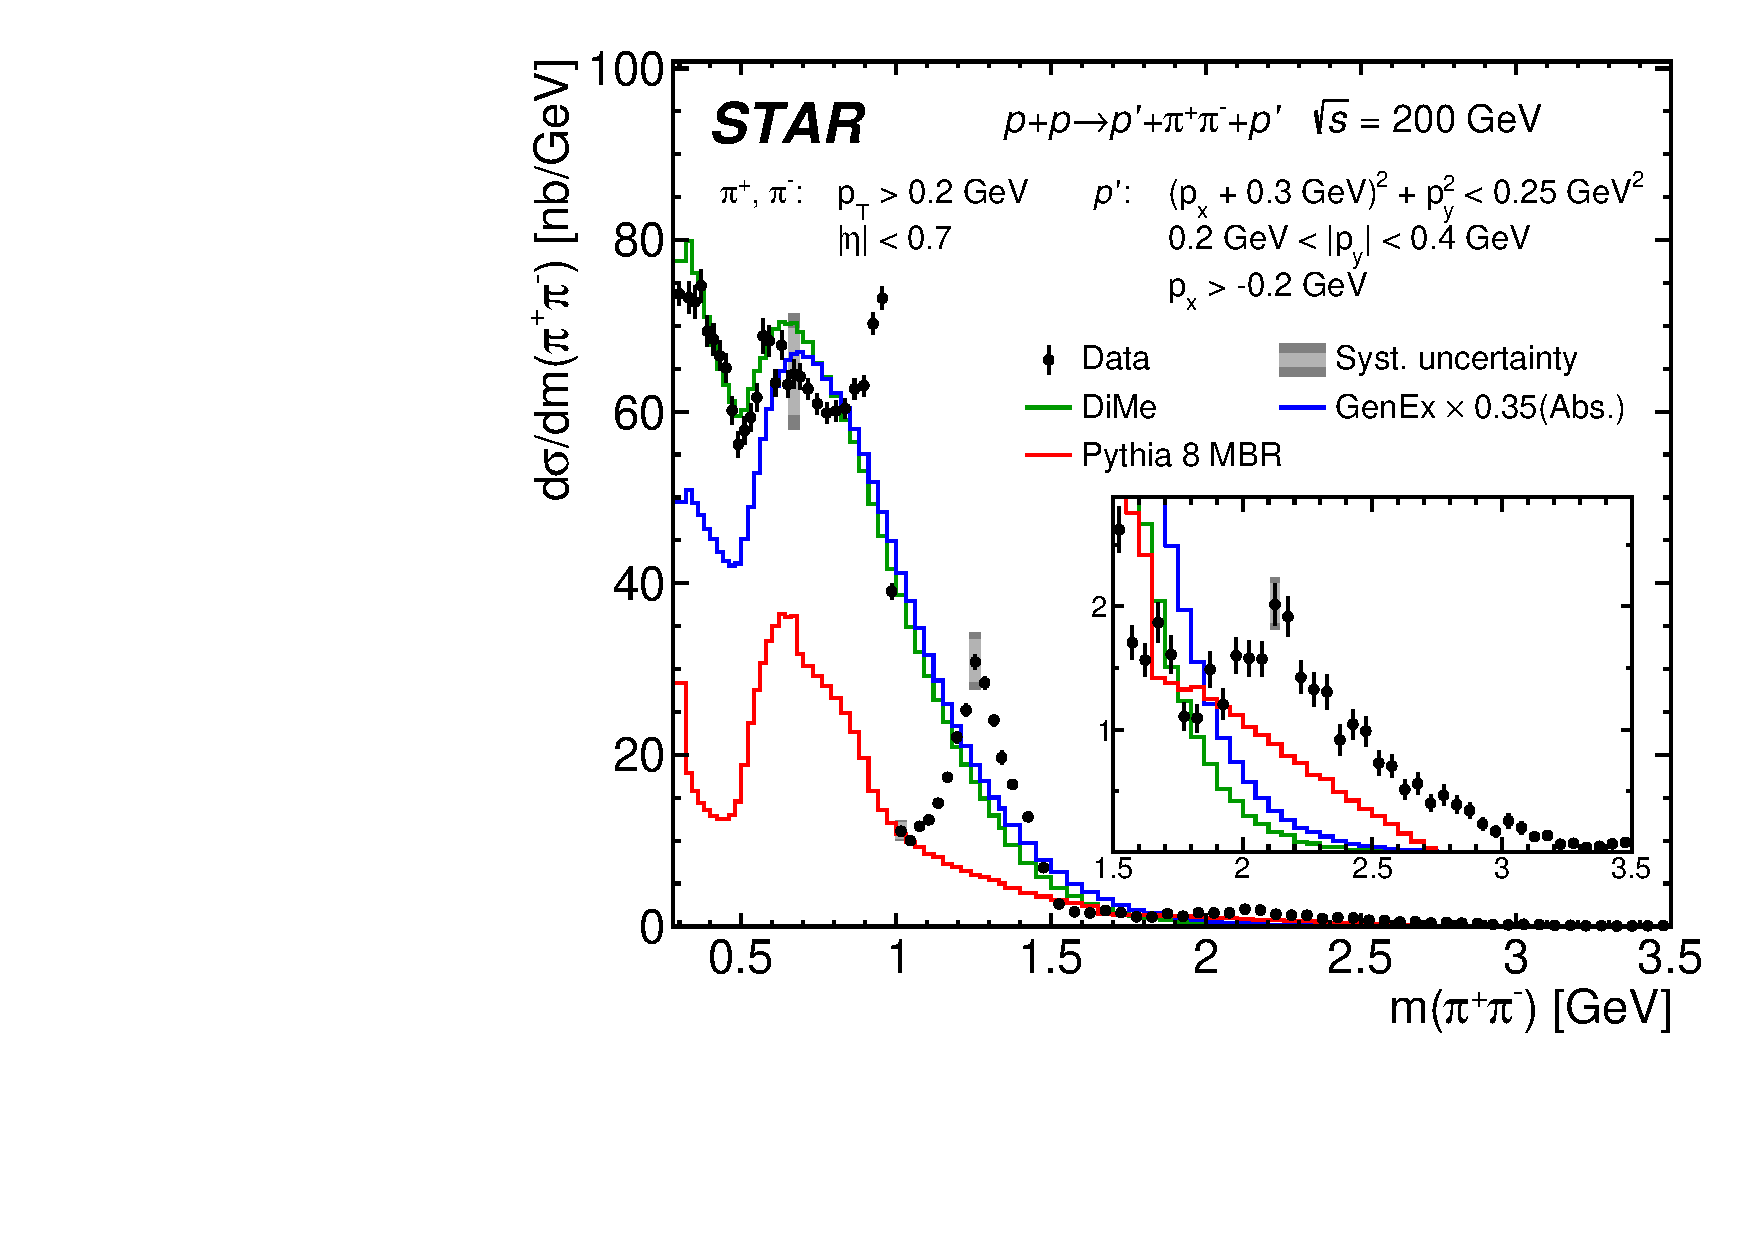
\includegraphics[width=.7\textwidth,page=1]{graphics/physicsResults/FinalResult_InvMass_pion.pdf}
%
\caption{Differential cross sections for CEP of charged particle pairs $\pi^+\pi^-$ as a function of the invariant mass of the pair in the fiducial region explained on the plots. Data are shown as solid points with error bars representing the statistical uncertainties. The typical systematic uncertainties are shown as gray boxes for only few data points as they are almost fully correlated between neighboring bins. Predictions from MC models GenEx, DiMe and MBR are shown as histograms. In the lower panels in the bottom plots the ratios of the MC predictions scaled to data and the data are shown.}
\label{results_01}
\end{figure}
%
\begin{figure}[h]
\centering
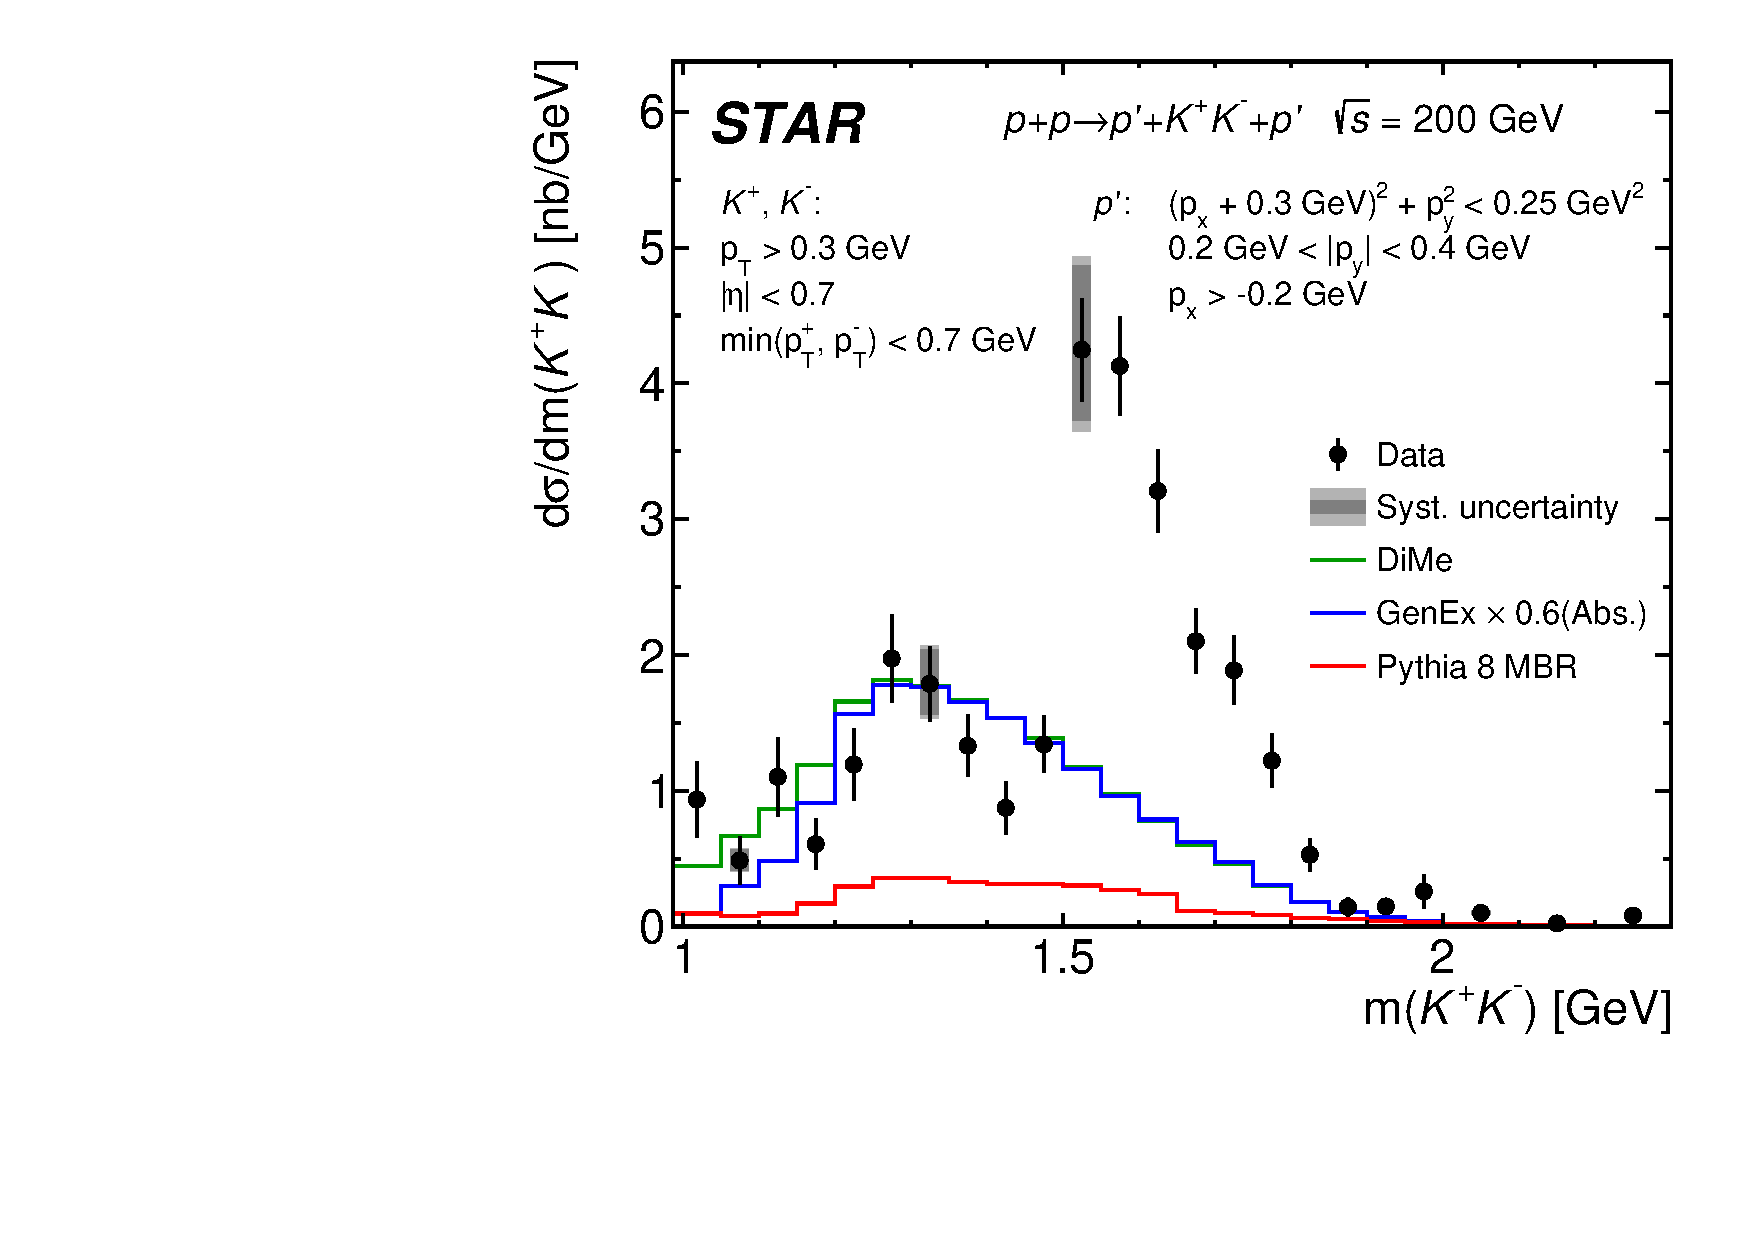
\includegraphics[width=.48\textwidth,page=1]{graphics/physicsResults/FinalResult_InvMass_kaon.pdf}
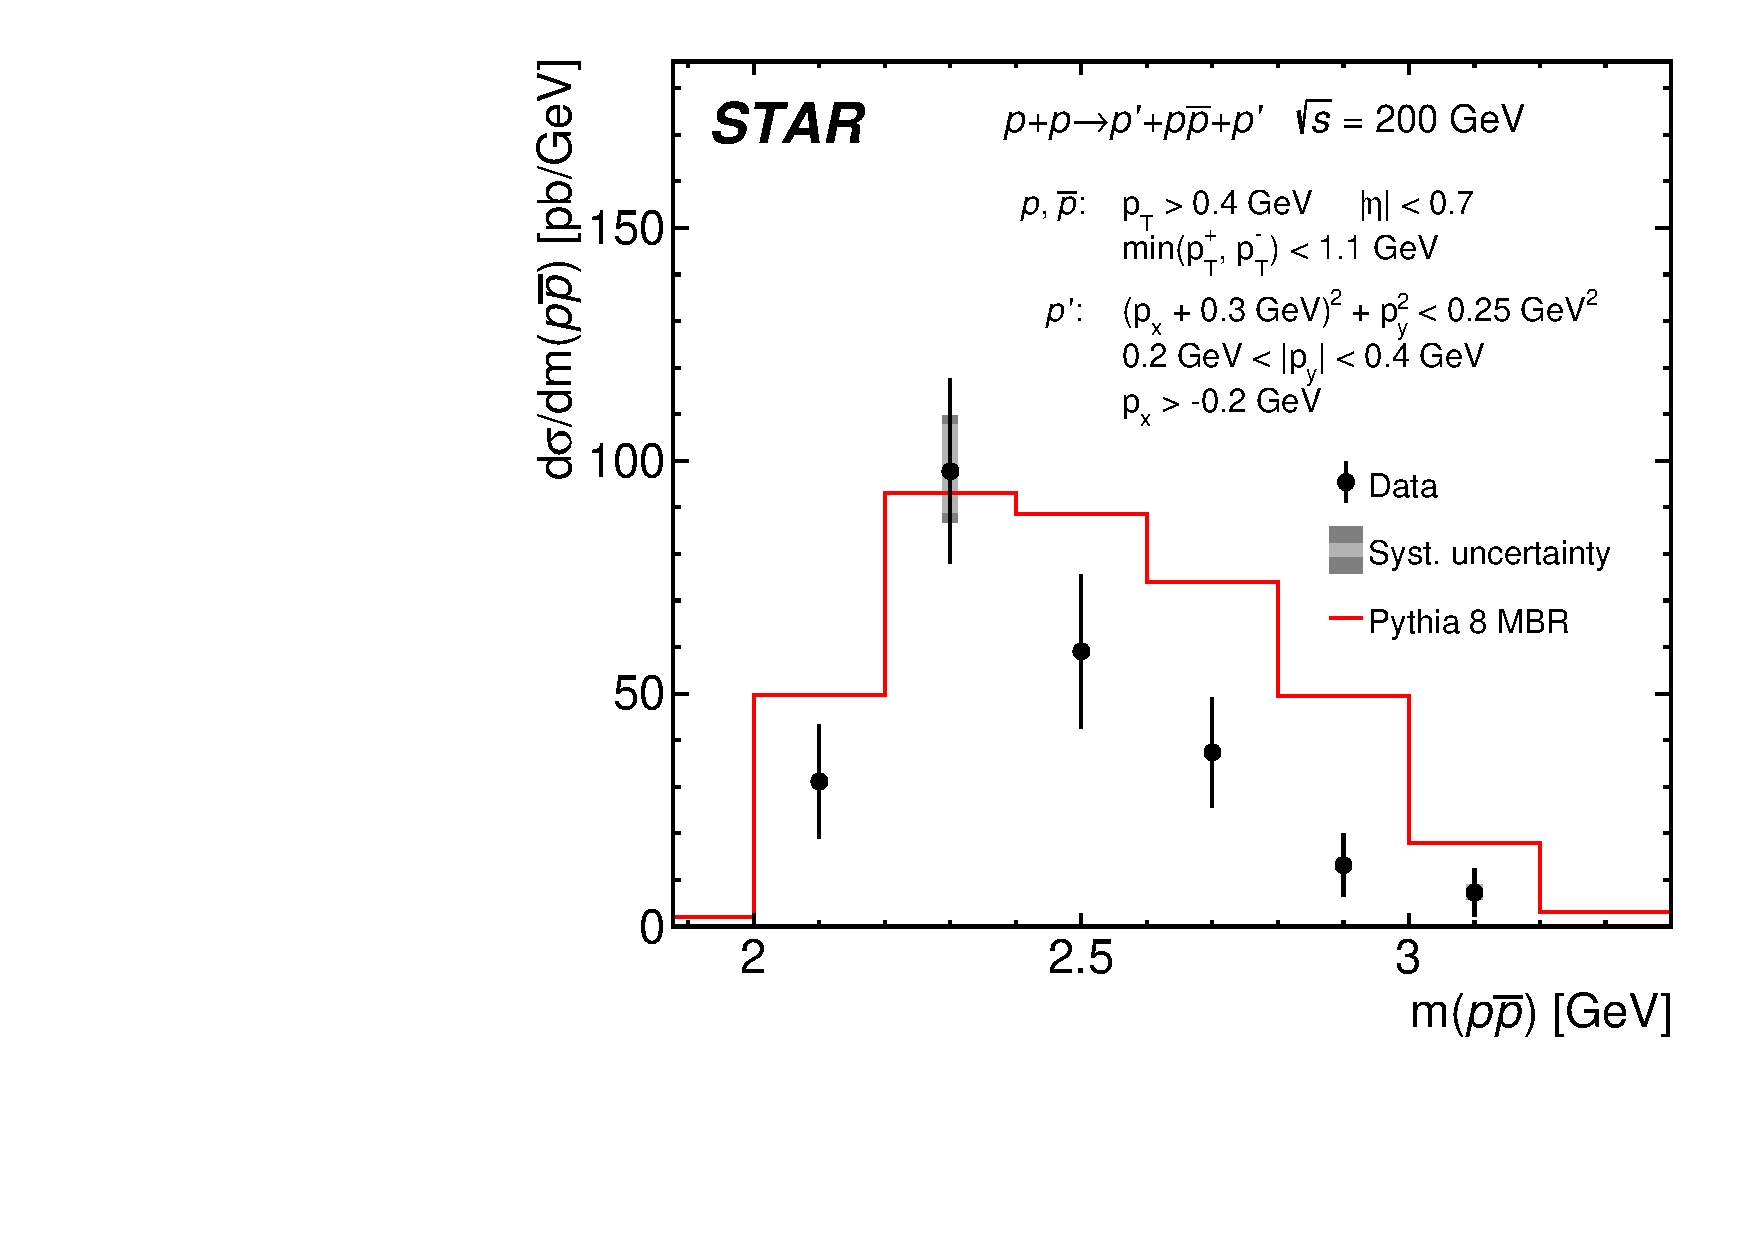
\includegraphics[width=.48\textwidth,page=1]{graphics/physicsResults/FinalResult_InvMass_proton.pdf}
%
\caption{Differential cross sections for CEP of charged particle pairs $K^+K^-$ (left) and $p\bar{p}$ (right) as a function of the invariant mass of the pair in the fiducial region explained on the plots. Data are shown as solid points with error bars representing the statistical uncertainties. The typical systematic uncertainties are shown as gray boxes for only few data points as they are almost fully correlated between neighboring bins. Predictions from MC models GenEx, DiMe and MBR are shown as histograms. In the lower panels in the bottom plots the ratios of the MC predictions scaled to data and the data are shown.}
\label{results_02}
\end{figure}
% 
\begin{figure}[h]
\centering
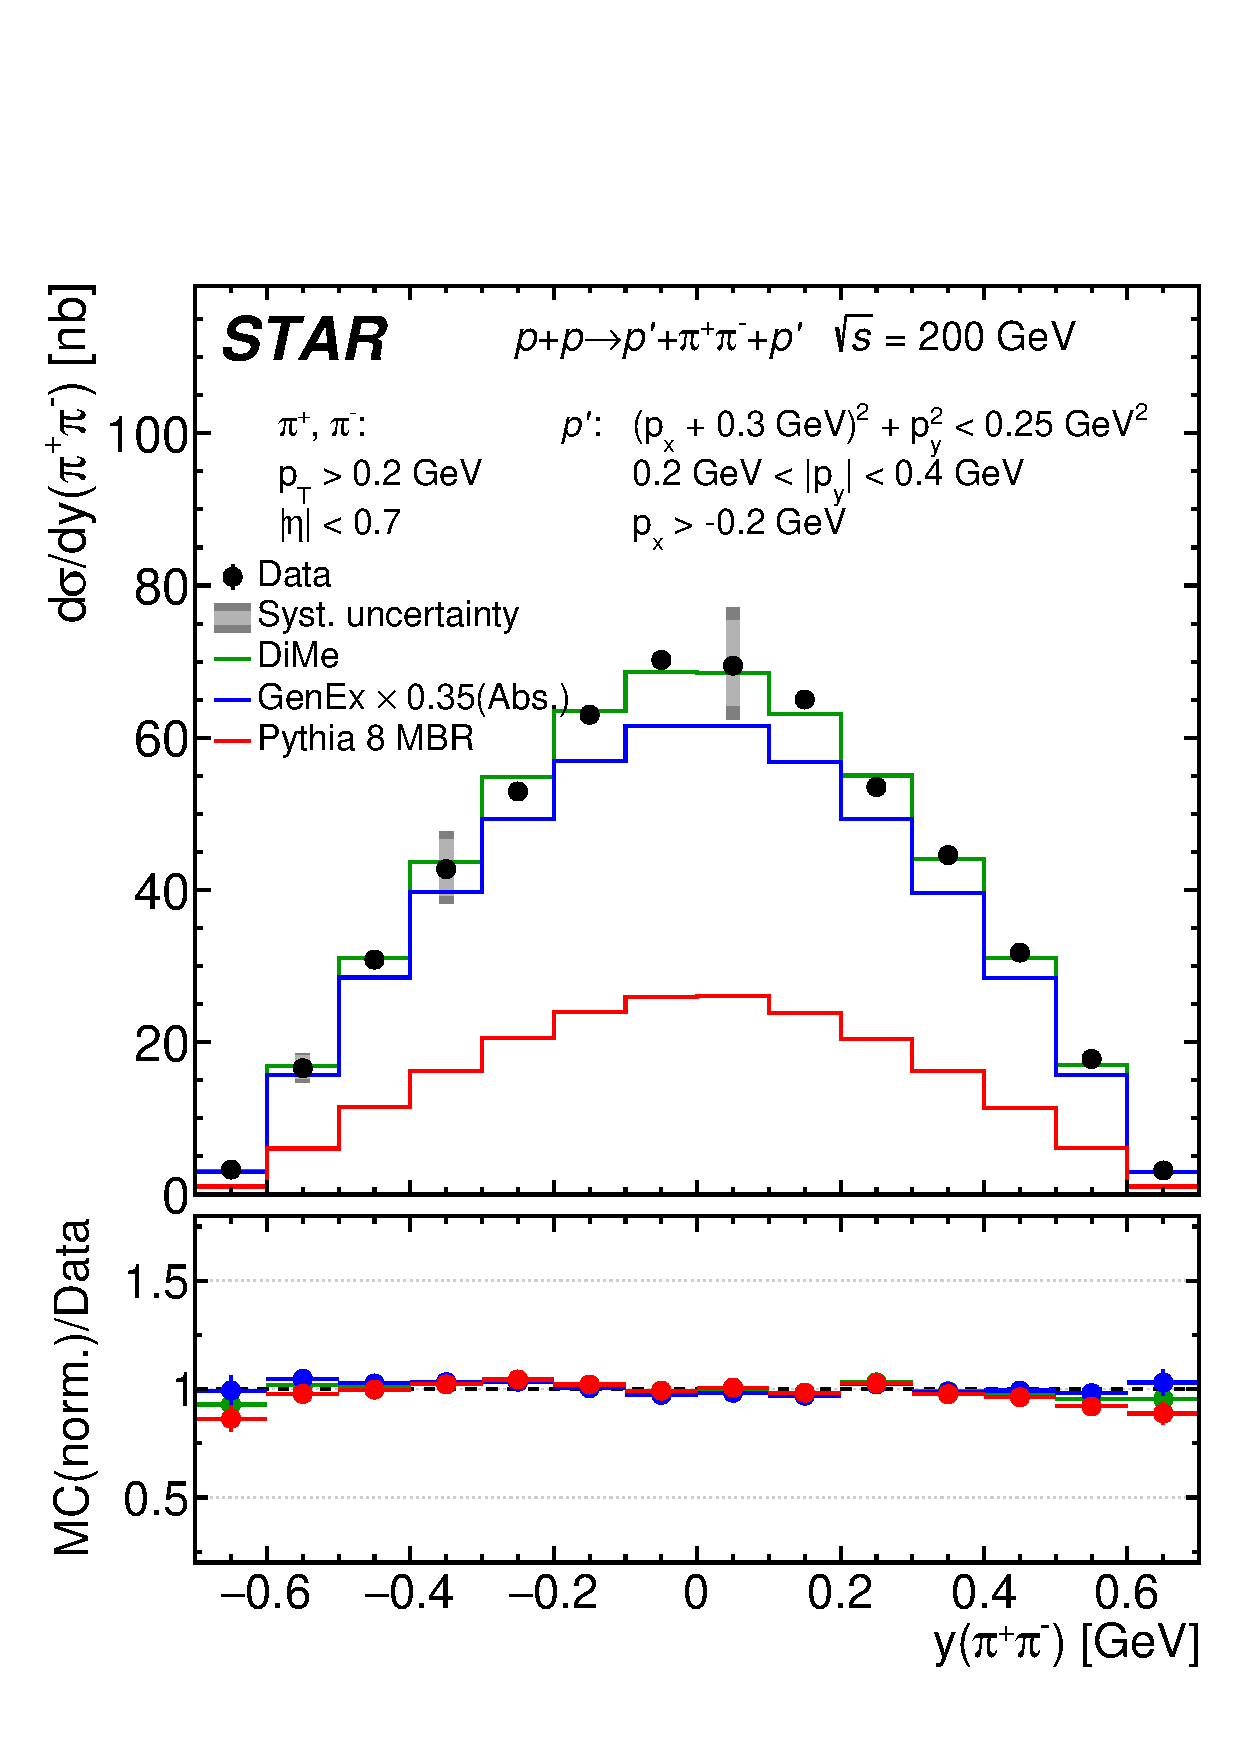
\includegraphics[width=.31\textwidth,page=1]{graphics/physicsResults/Ratio_FinalResult_Rapidity_pion.pdf}
\hfill
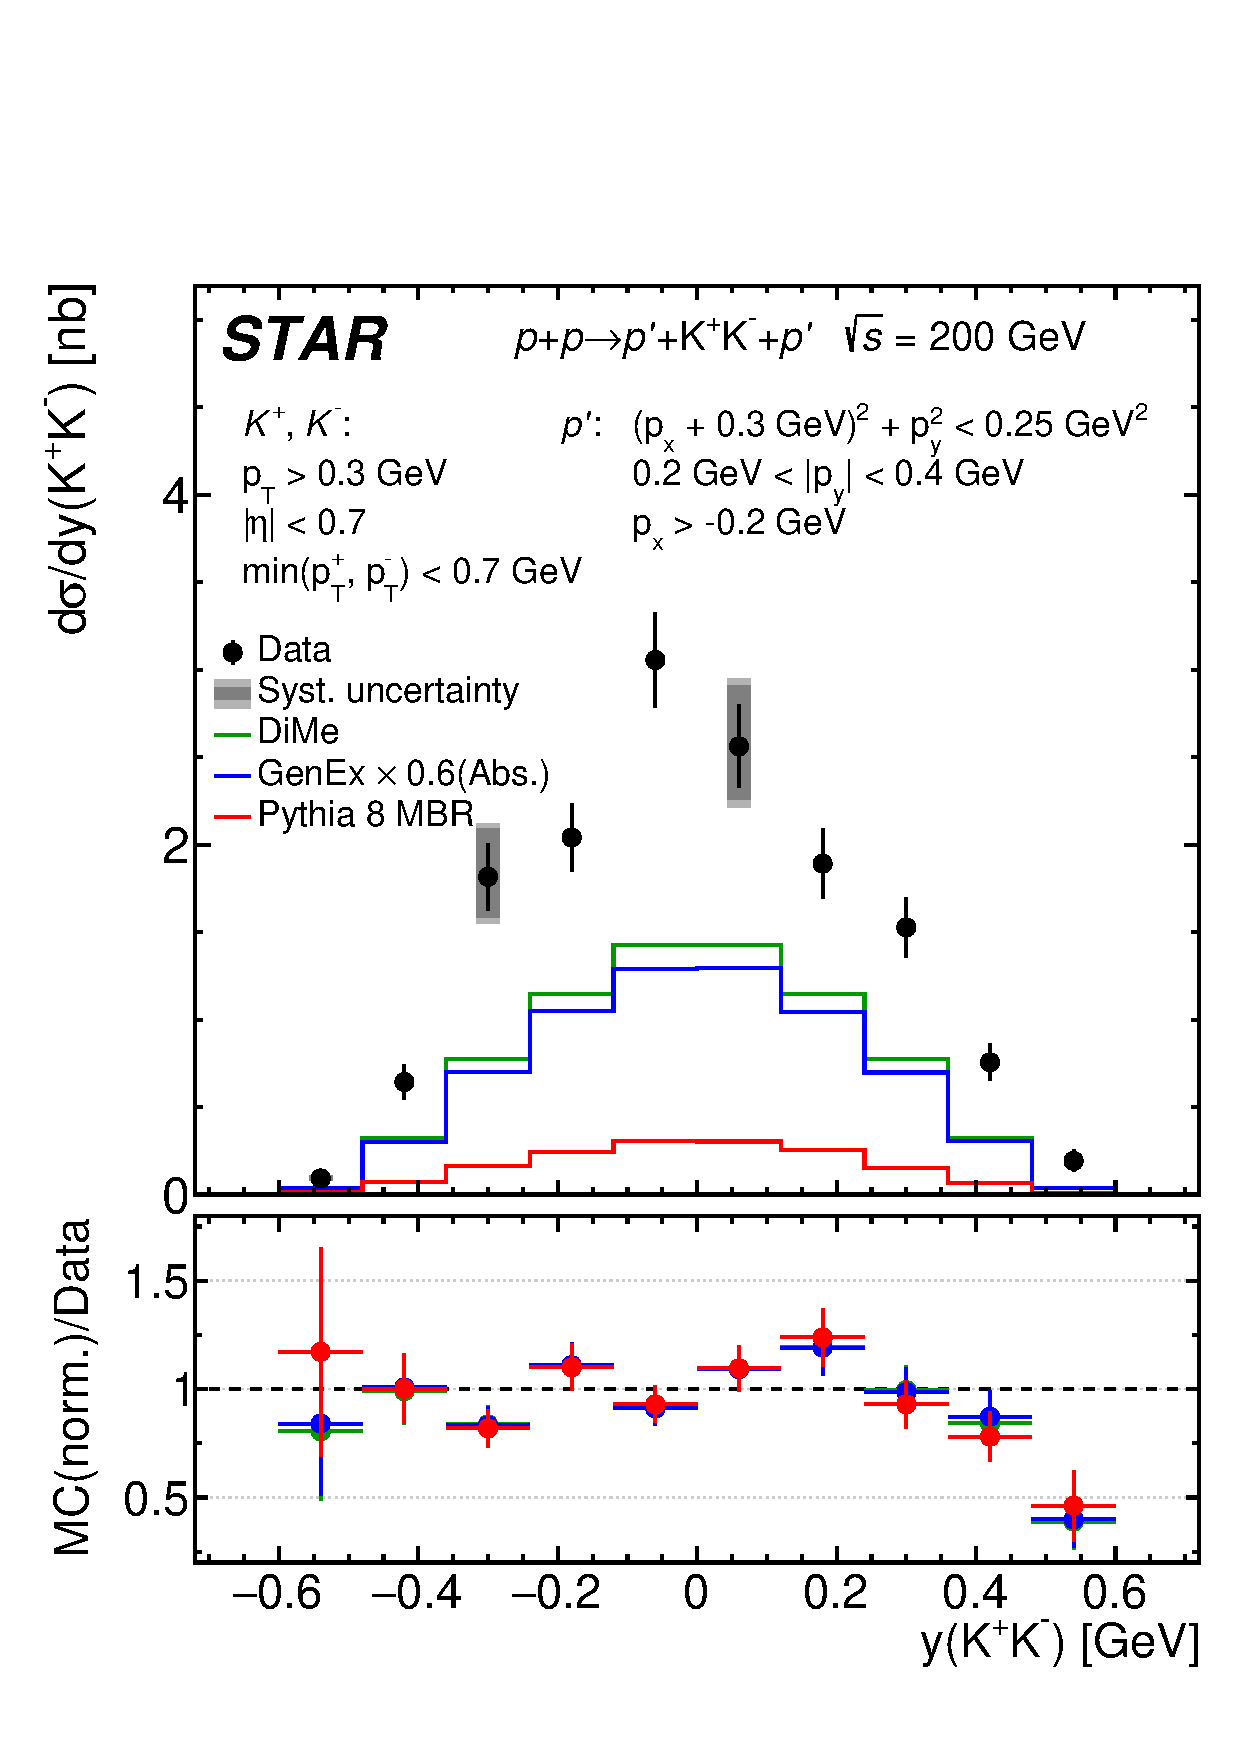
\includegraphics[width=.31\textwidth,page=1]{graphics/physicsResults/Ratio_FinalResult_Rapidity_kaon.pdf}
\hfill
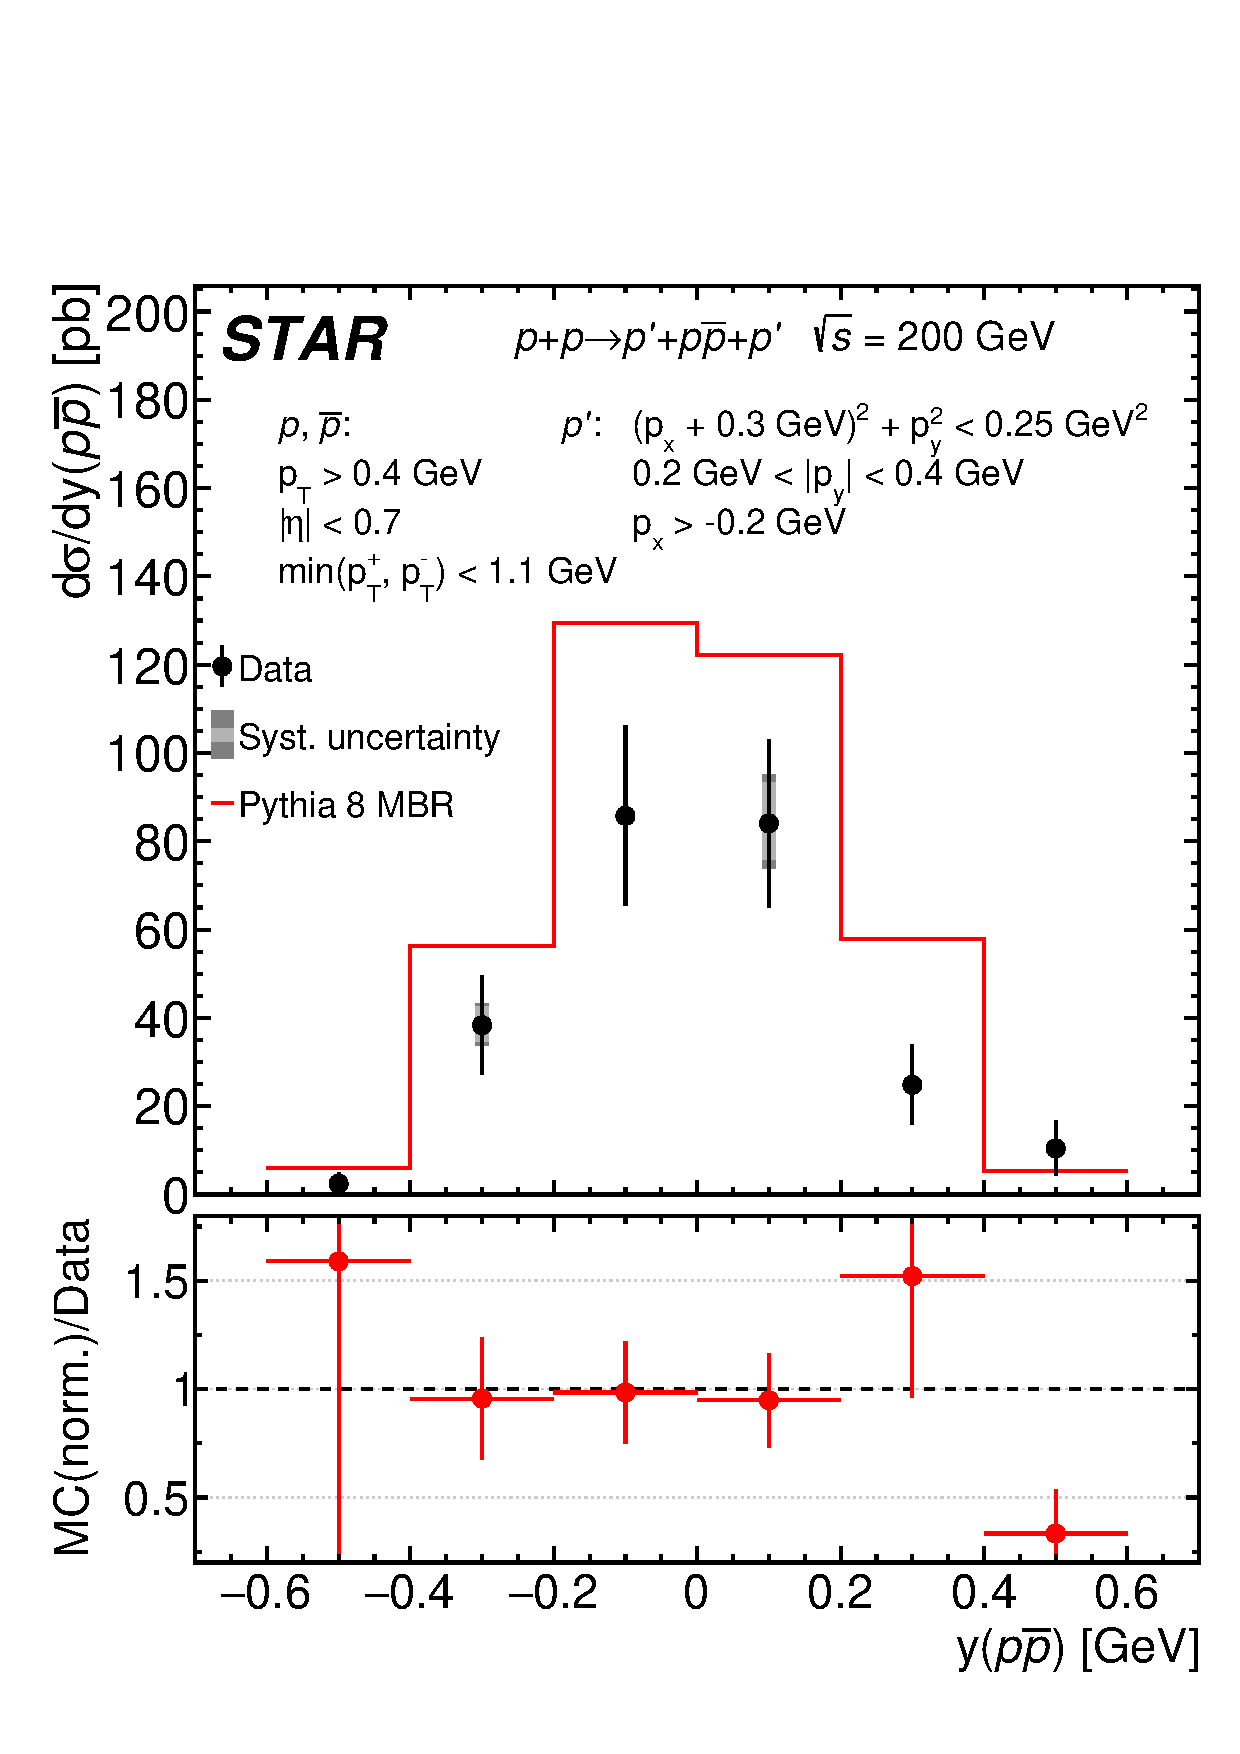
\includegraphics[width=.31\textwidth,page=1]{graphics/physicsResults/Ratio_FinalResult_Rapidity_proton.pdf}
%
\caption{Differential cross sections for CEP of charged particle pairs $\pi^+\pi^-$ (let), $K^+K^-$ (middle) and $p\bar{p}$ (right) as a function of the pair rapidity measured in the fiducial region explained on the plots. Data are shown as solid points with error bars representing the statistical uncertainties. The typical systematic uncertainties are shown as gray boxes for only few data points as they are almost fully correlated between neighboring bins. Predictions from MC models GenEx, DiMe and MBR are shown as histograms. In the lower panels in the bottom plots the ratios of the MC predictions scaled to data and the data are shown.}
\label{results_1}
\end{figure}
%
% \indent
% Figure~\ref{results_2}(right column) shows the differential cross sections for CEP of different particle species pairs as a function of the sum of the squares of the four-momenta transfers at the proton vertices.
% %
% The shapes of measured cross sections are strongly affected by the fiducial cuts applied to the forward scattered protons.
% %
% The shapes of the differential cross sections for both $\pi^+\pi^-$ snd $K^+K^-$ pairs production are better described by the DiMe model than by GenEx and MBR models.
% In case of the cross section for $p\bar{p}$ pairs production the MBR model implemented in PYTHIA8 describes normalization of the data fairly well but predicts a steeper slope.\\
% %
% \indent
% Figure~\ref{results_3} shows the differential cross sections for CEP of different particle species pairs as a function of the pair invariant mass separately in two $\Delta\phi$ regions: $\Delta\phi<90$ degree (left column) and $\Delta\phi>90$ degree (right column).
% %
% Sharp drops of the measured cross sections at $m(\pi^+\pi^-) < 0.6$~GeV and at $m(K^+K^-) < 1.3$~GeV for the $\Delta\phi>$ 90 degree range are due to the fiducial cuts applied to the forward scattered protons. 
% %
% In case of the cross section for CEP of $\pi^+\pi^-$ pairs in $\Delta\phi<90$ degree range the peak around $f_2(1270)$ resonance in data is significantly suppressed while the peak at $f_0(980)$ is enhanced as well as possible resonances in the mass range $1.3-1.5$ MeV compared to the $\Delta\phi>90$ degrees range. 
%
\begin{figure}[h]
\centering
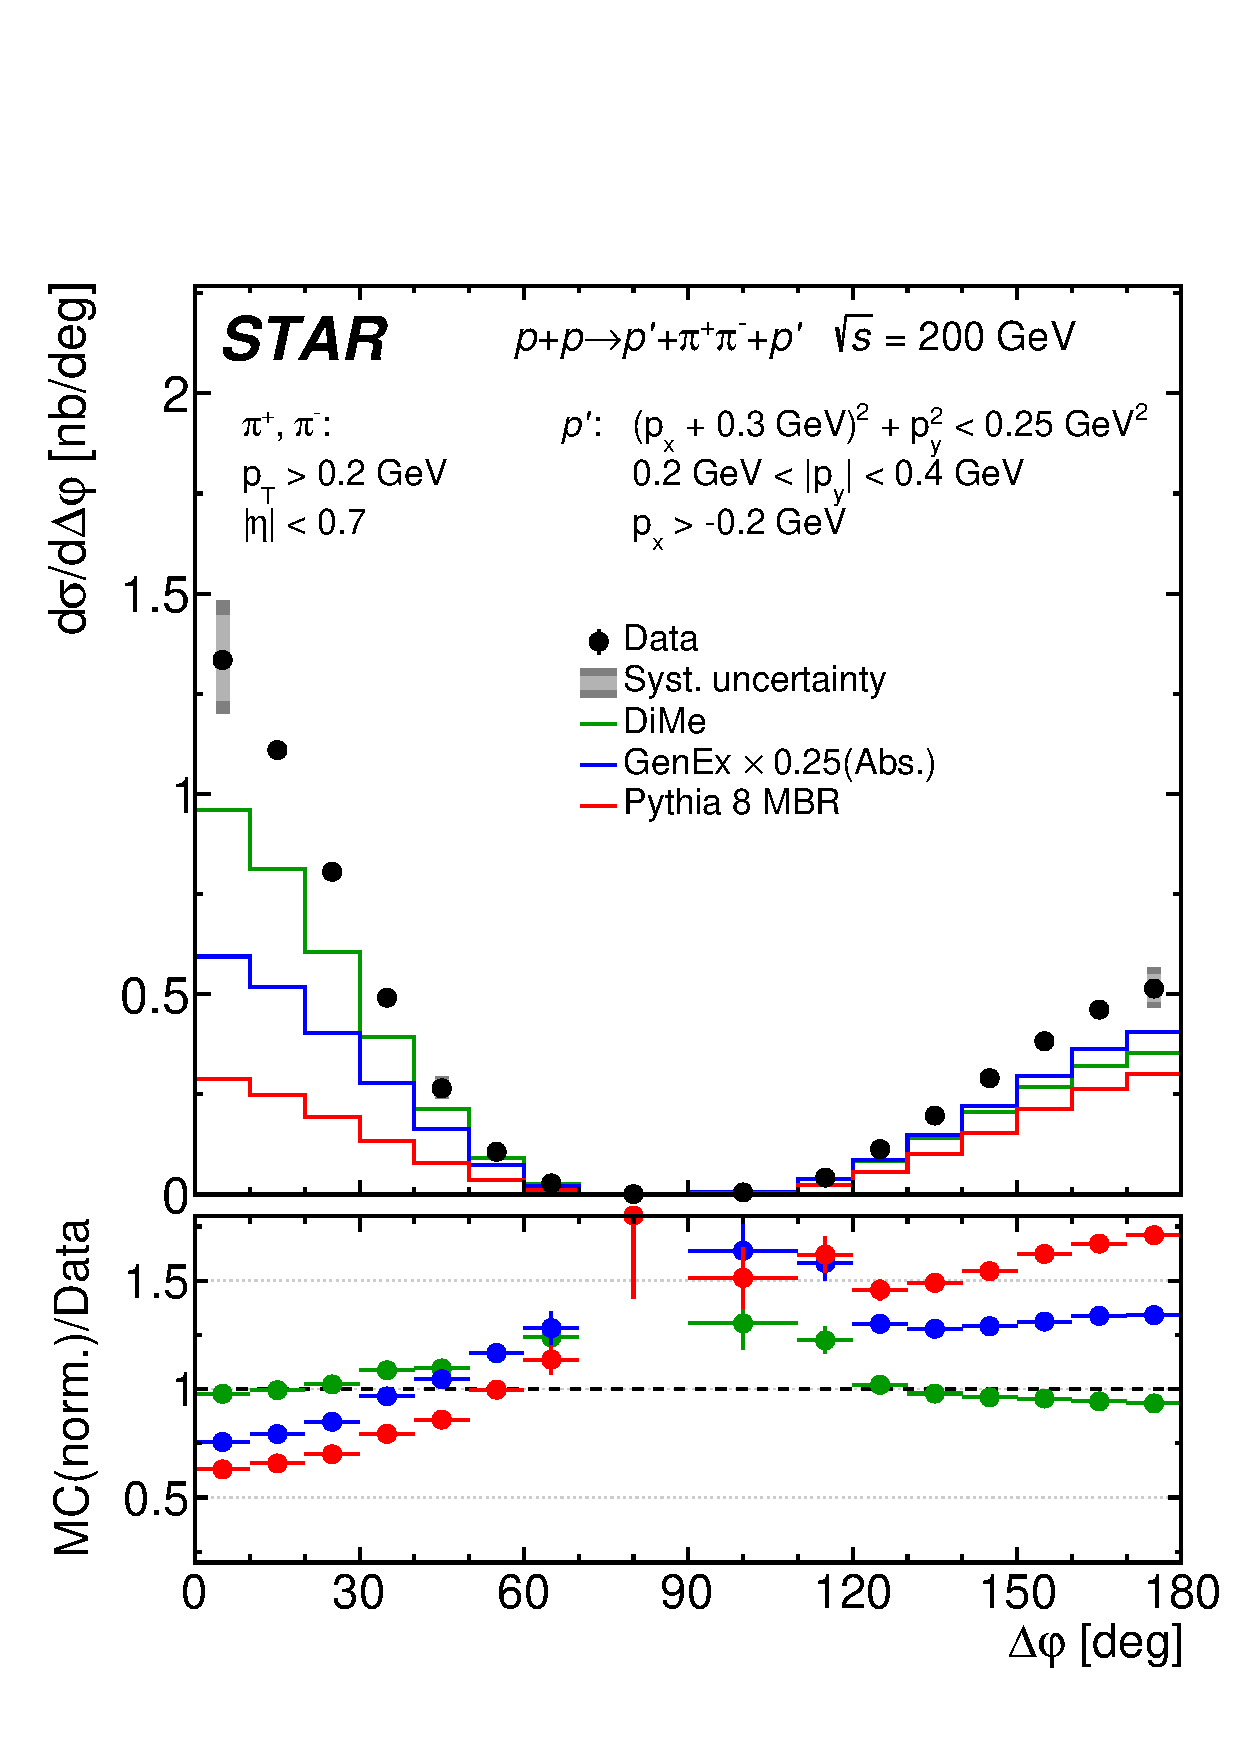
\includegraphics[width=.31\textwidth,page=1]{graphics/physicsResults/Ratio_FinalResult_DeltaPhi_pion.pdf}
\hfill
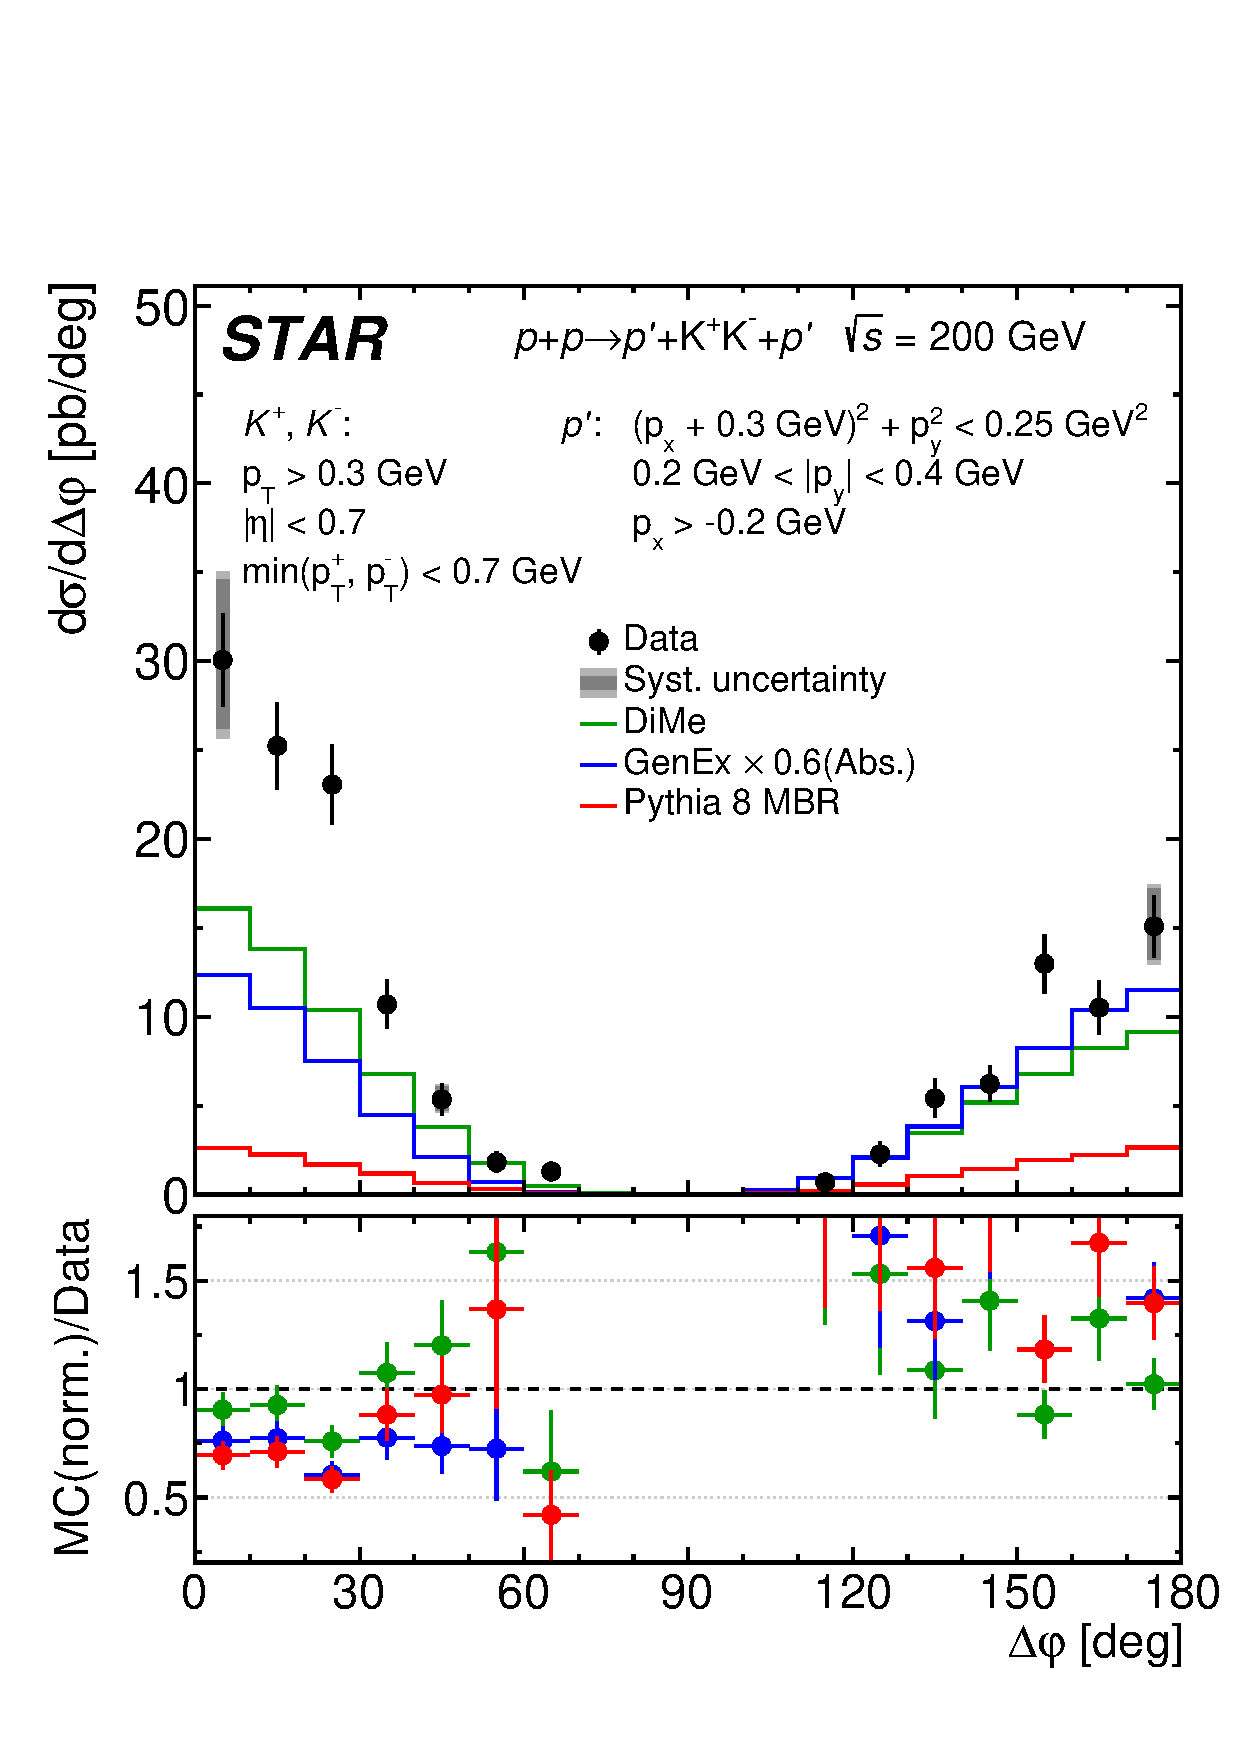
\includegraphics[width=.31\textwidth,page=1]{graphics/physicsResults/Ratio_FinalResult_DeltaPhi_kaon.pdf}
\hfill
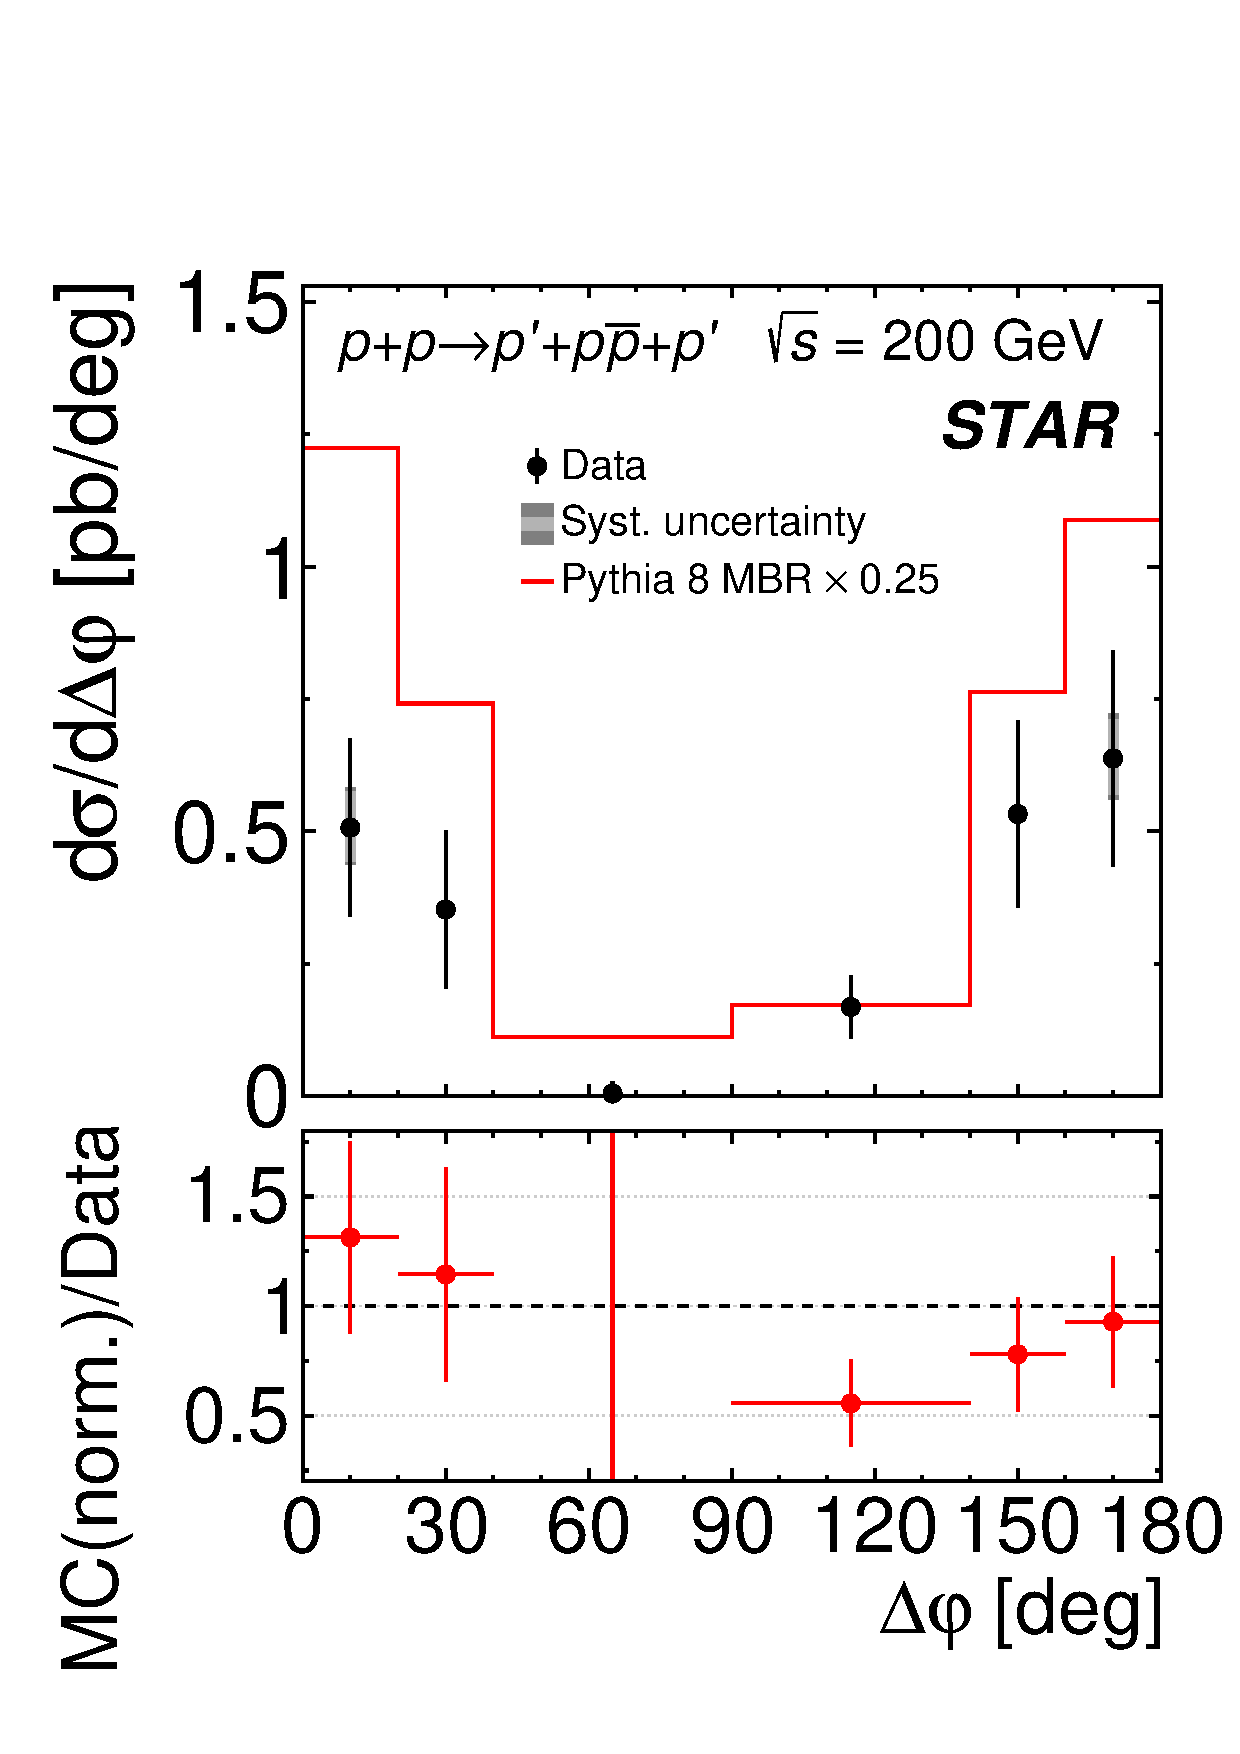
\includegraphics[width=.31\textwidth,page=1]{graphics/physicsResults/Ratio_FinalResult_DeltaPhi_proton.pdf}
\newline
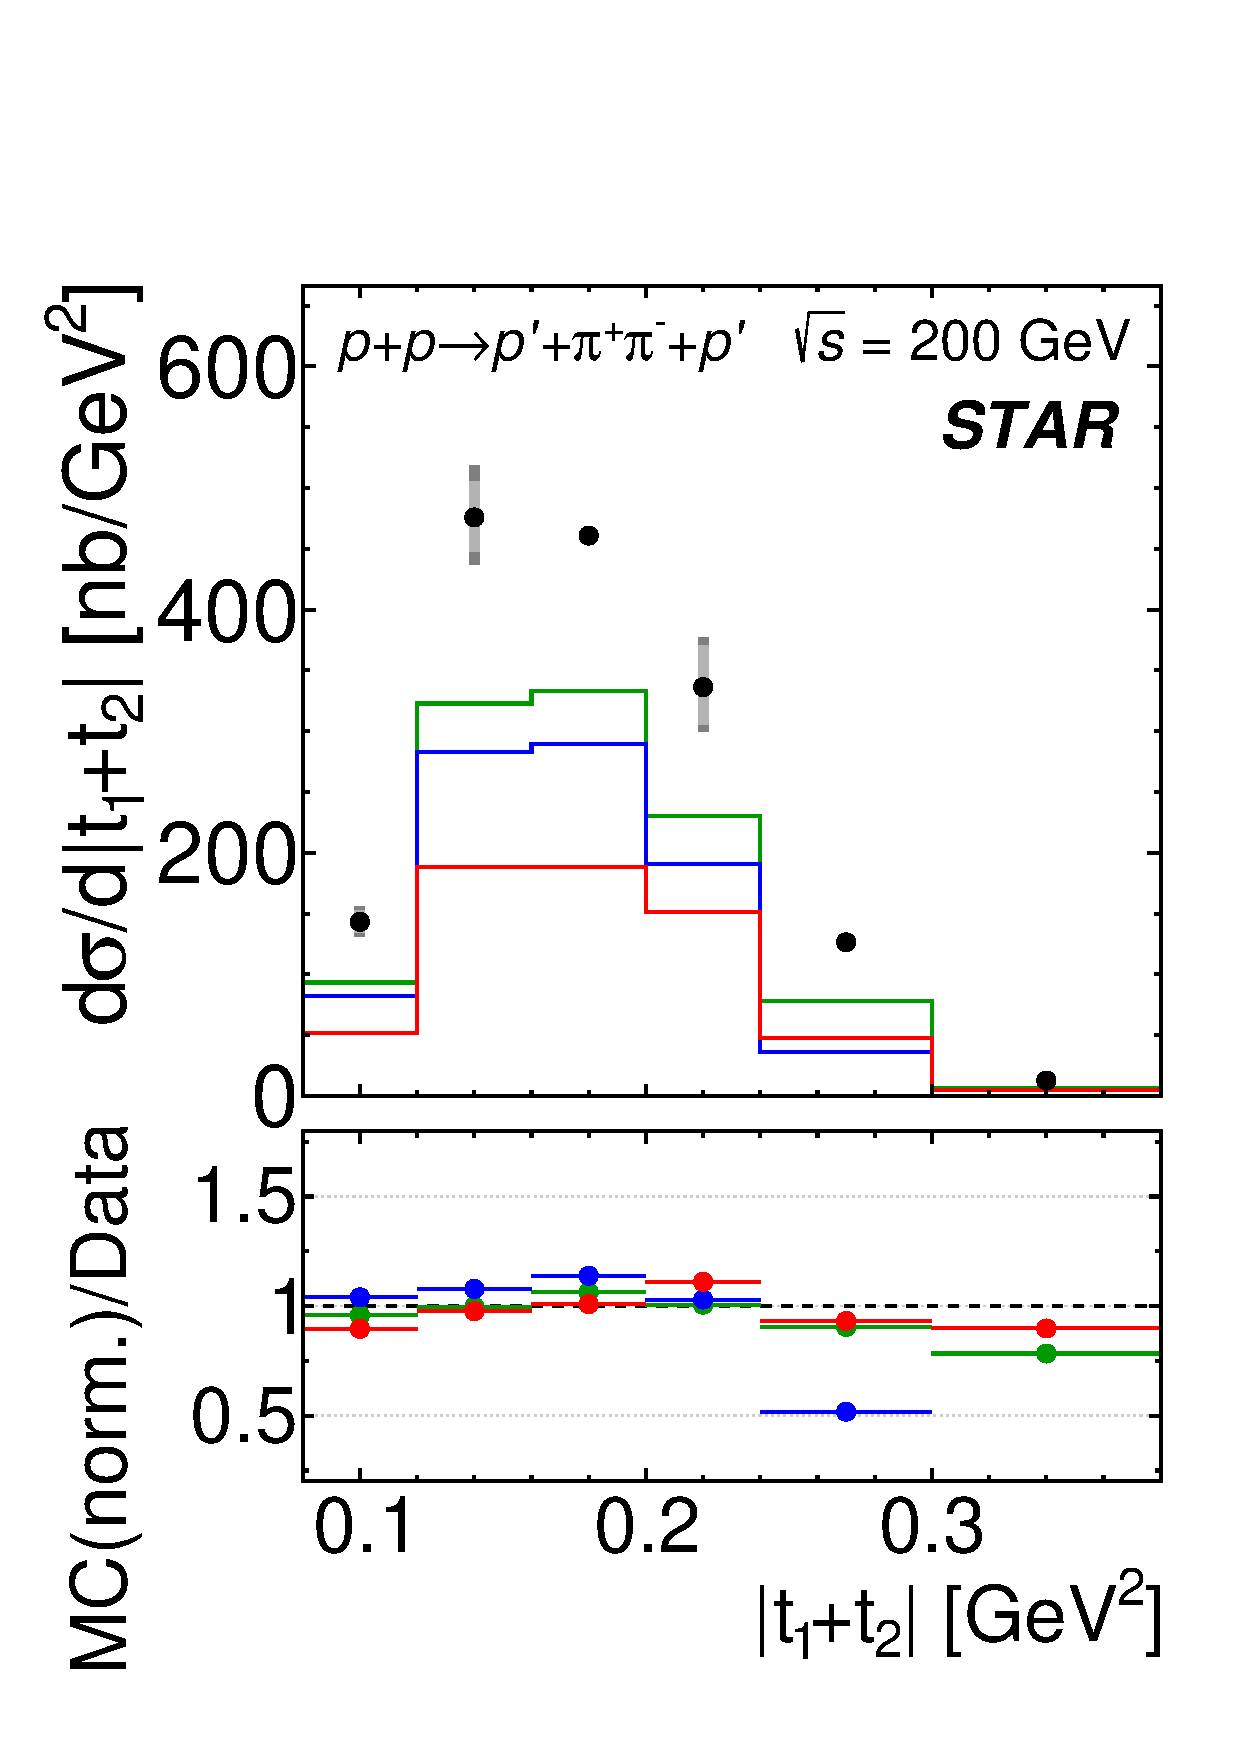
\includegraphics[width=.31\textwidth,page=1]{graphics/physicsResults/Ratio_FinalResult_MandelstamTSum_pion.pdf}
\hfill
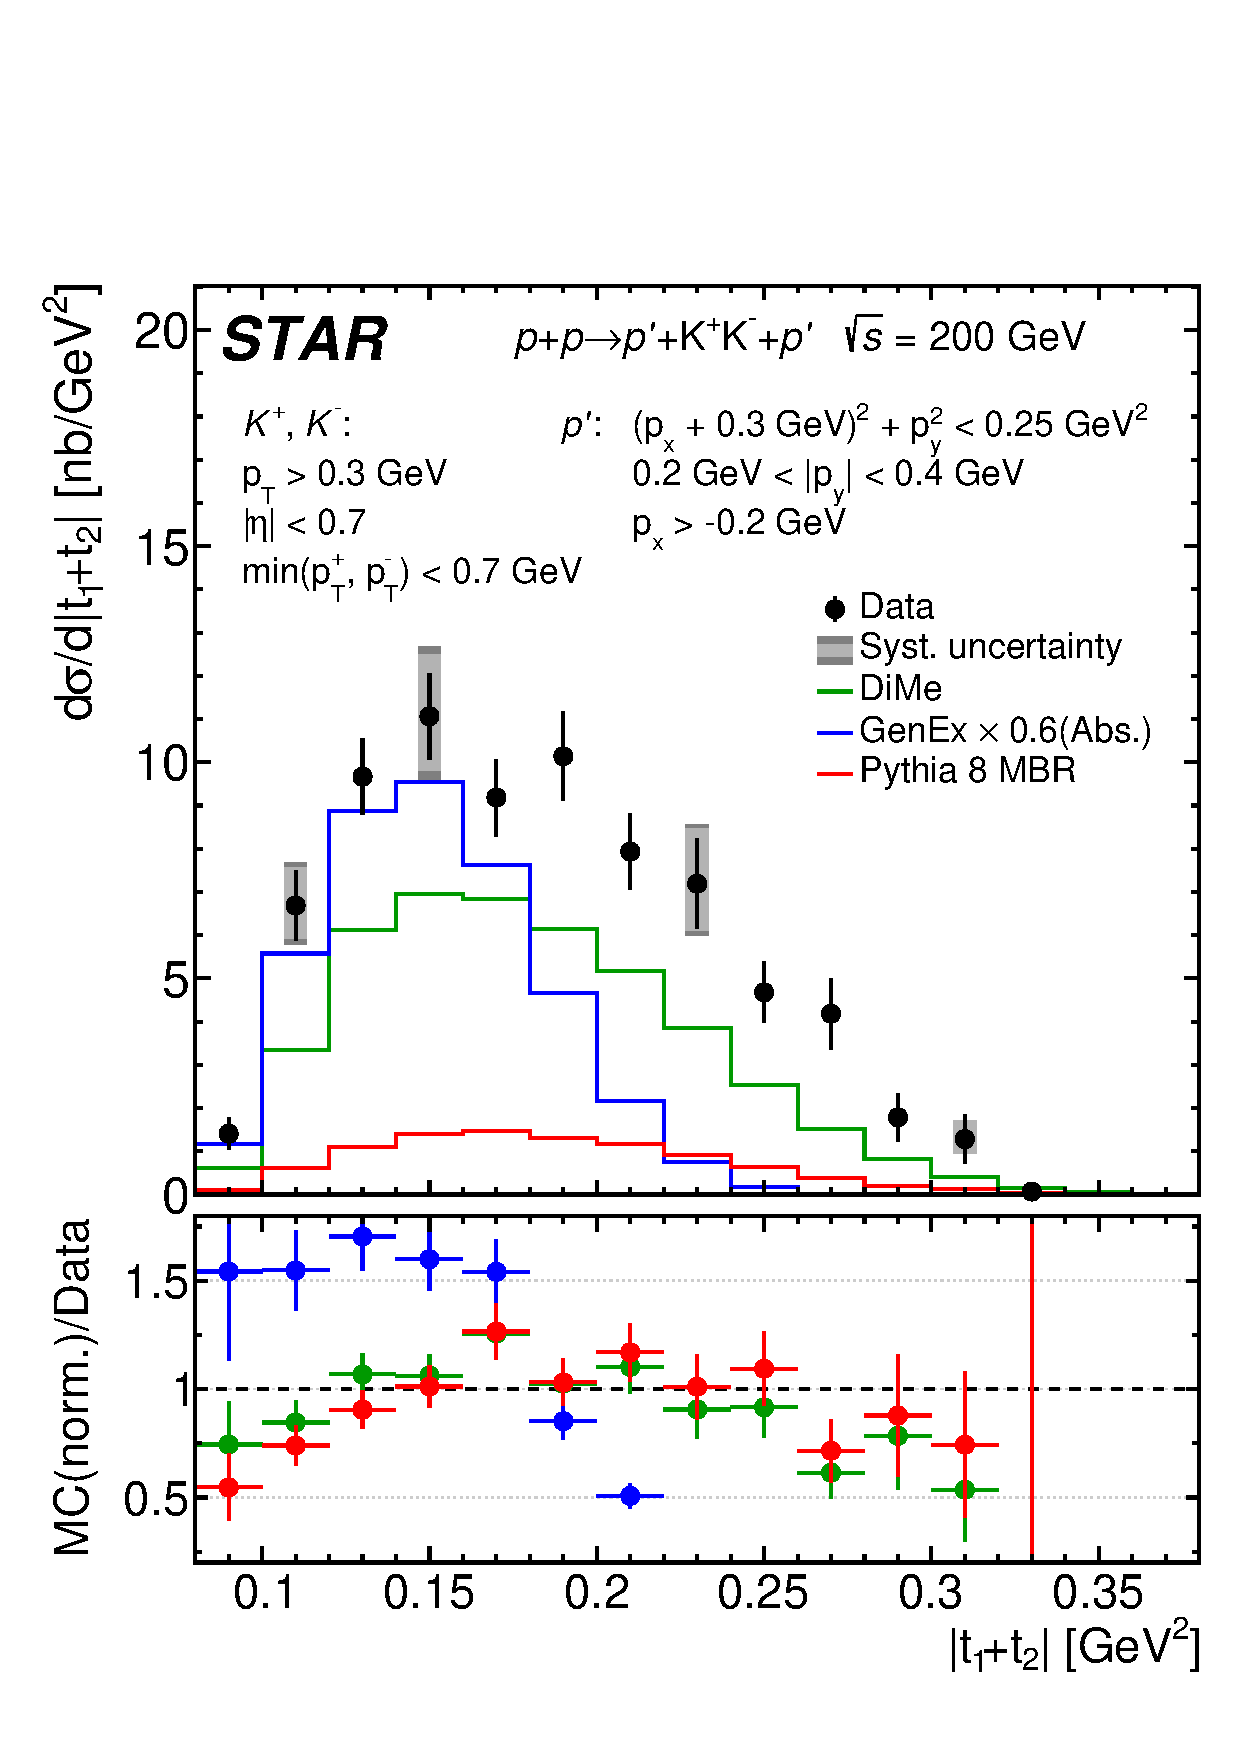
\includegraphics[width=.31\textwidth,page=1]{graphics/physicsResults/Ratio_FinalResult_MandelstamTSum_kaon.pdf}
\hfill
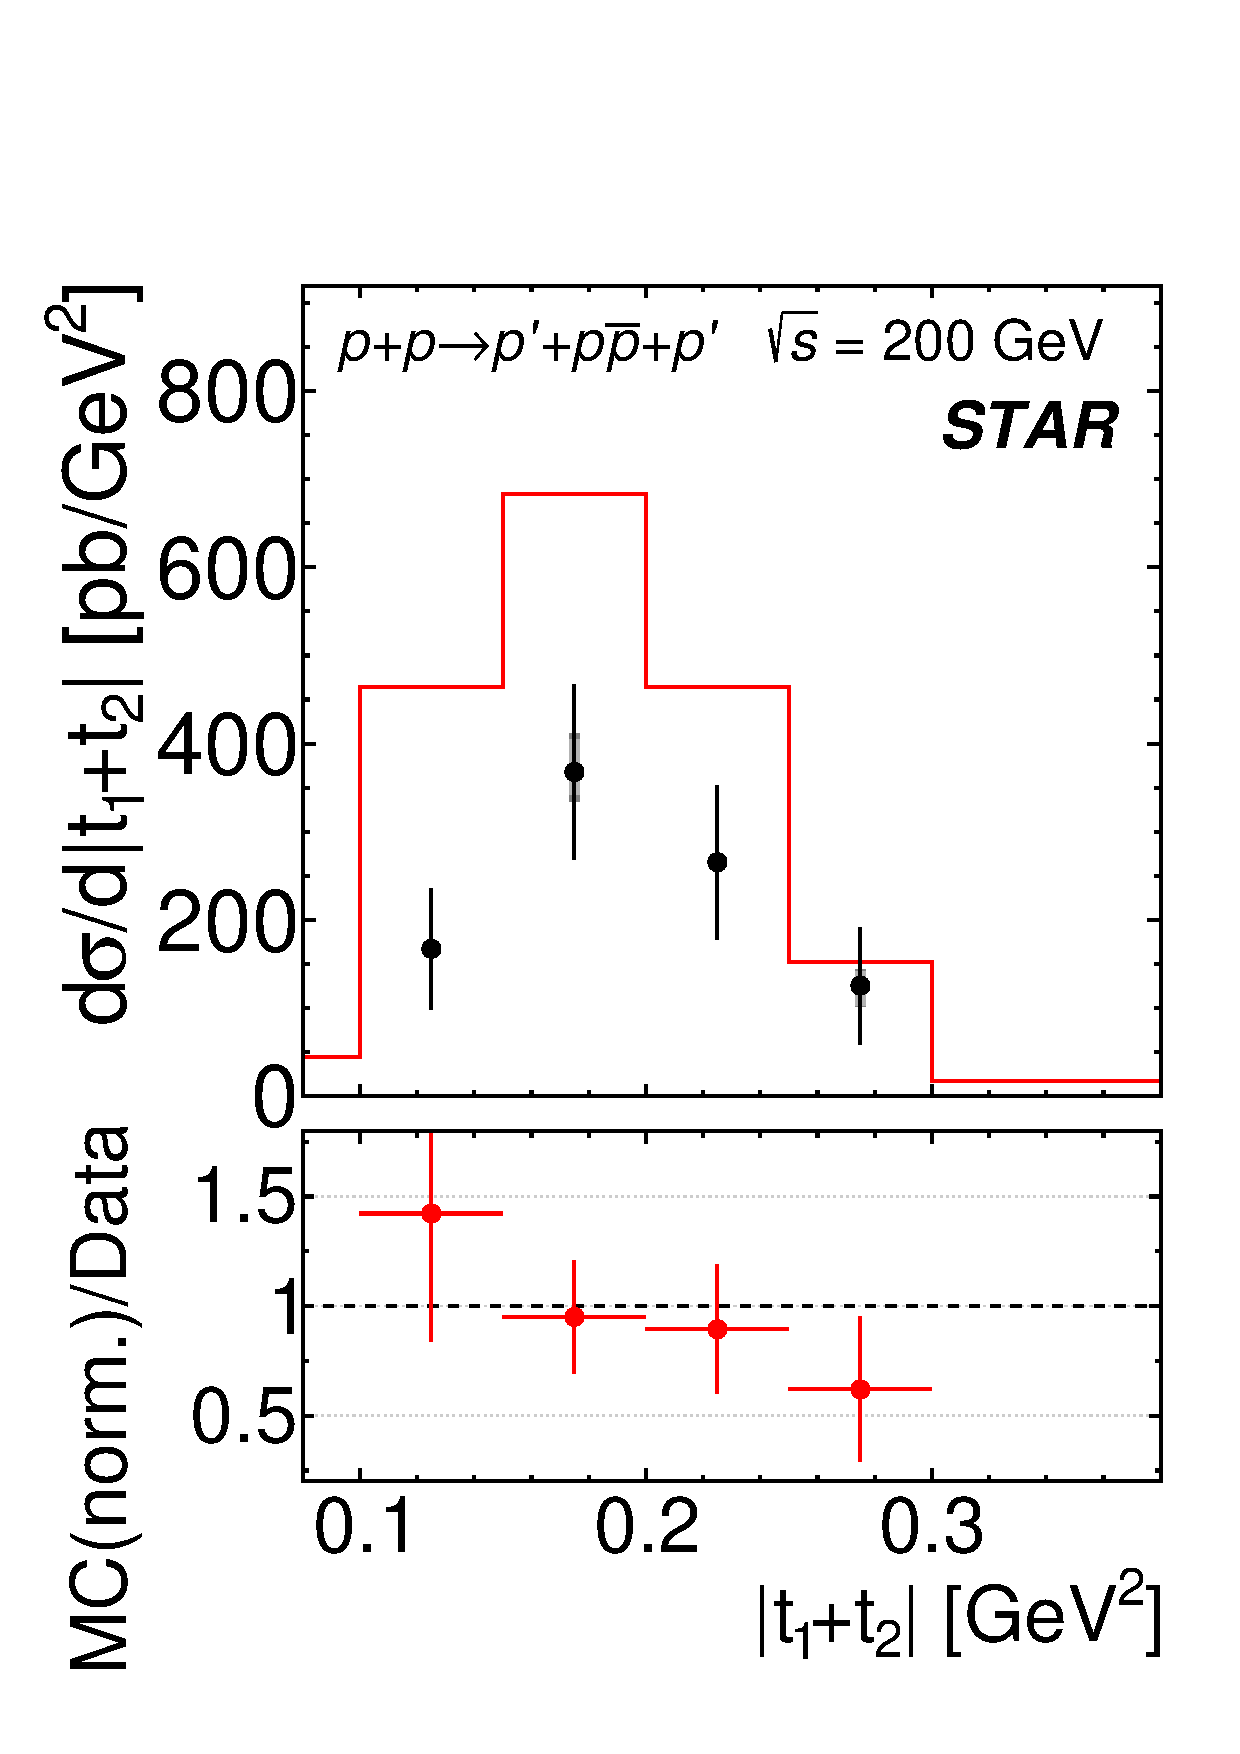
\includegraphics[width=.31\textwidth,page=1]{graphics/physicsResults/Ratio_FinalResult_MandelstamTSum_proton.pdf}
%
\caption{Differential cross sections for CEP of charged particle pairs $\pi^+\pi^-$ (left column), $K^+K^-$ (middle column) and $p\bar{p}$ (right column) as a function of the difference of azimuthal angles of the forward scattered protons (top) and of the sum of the squares of the four-momenta losses in the proton vertices (bottom) measured in the fiducial region explained on the plots. Data are shown as solid points with error bars representing the statistical uncertainties. The typical systematic uncertainties are shown as gray boxes for only few data points as they are almost fully correlated between neighboring bins. Predictions from MC models GenEx, DiMe and MBR are shown as histograms. In the lower panels the ratios of the MC predictions scaled to data and the data are shown.}
\label{results_2}
\end{figure}
%
\begin{figure}[h]
\centering
\hspace*{5pt}
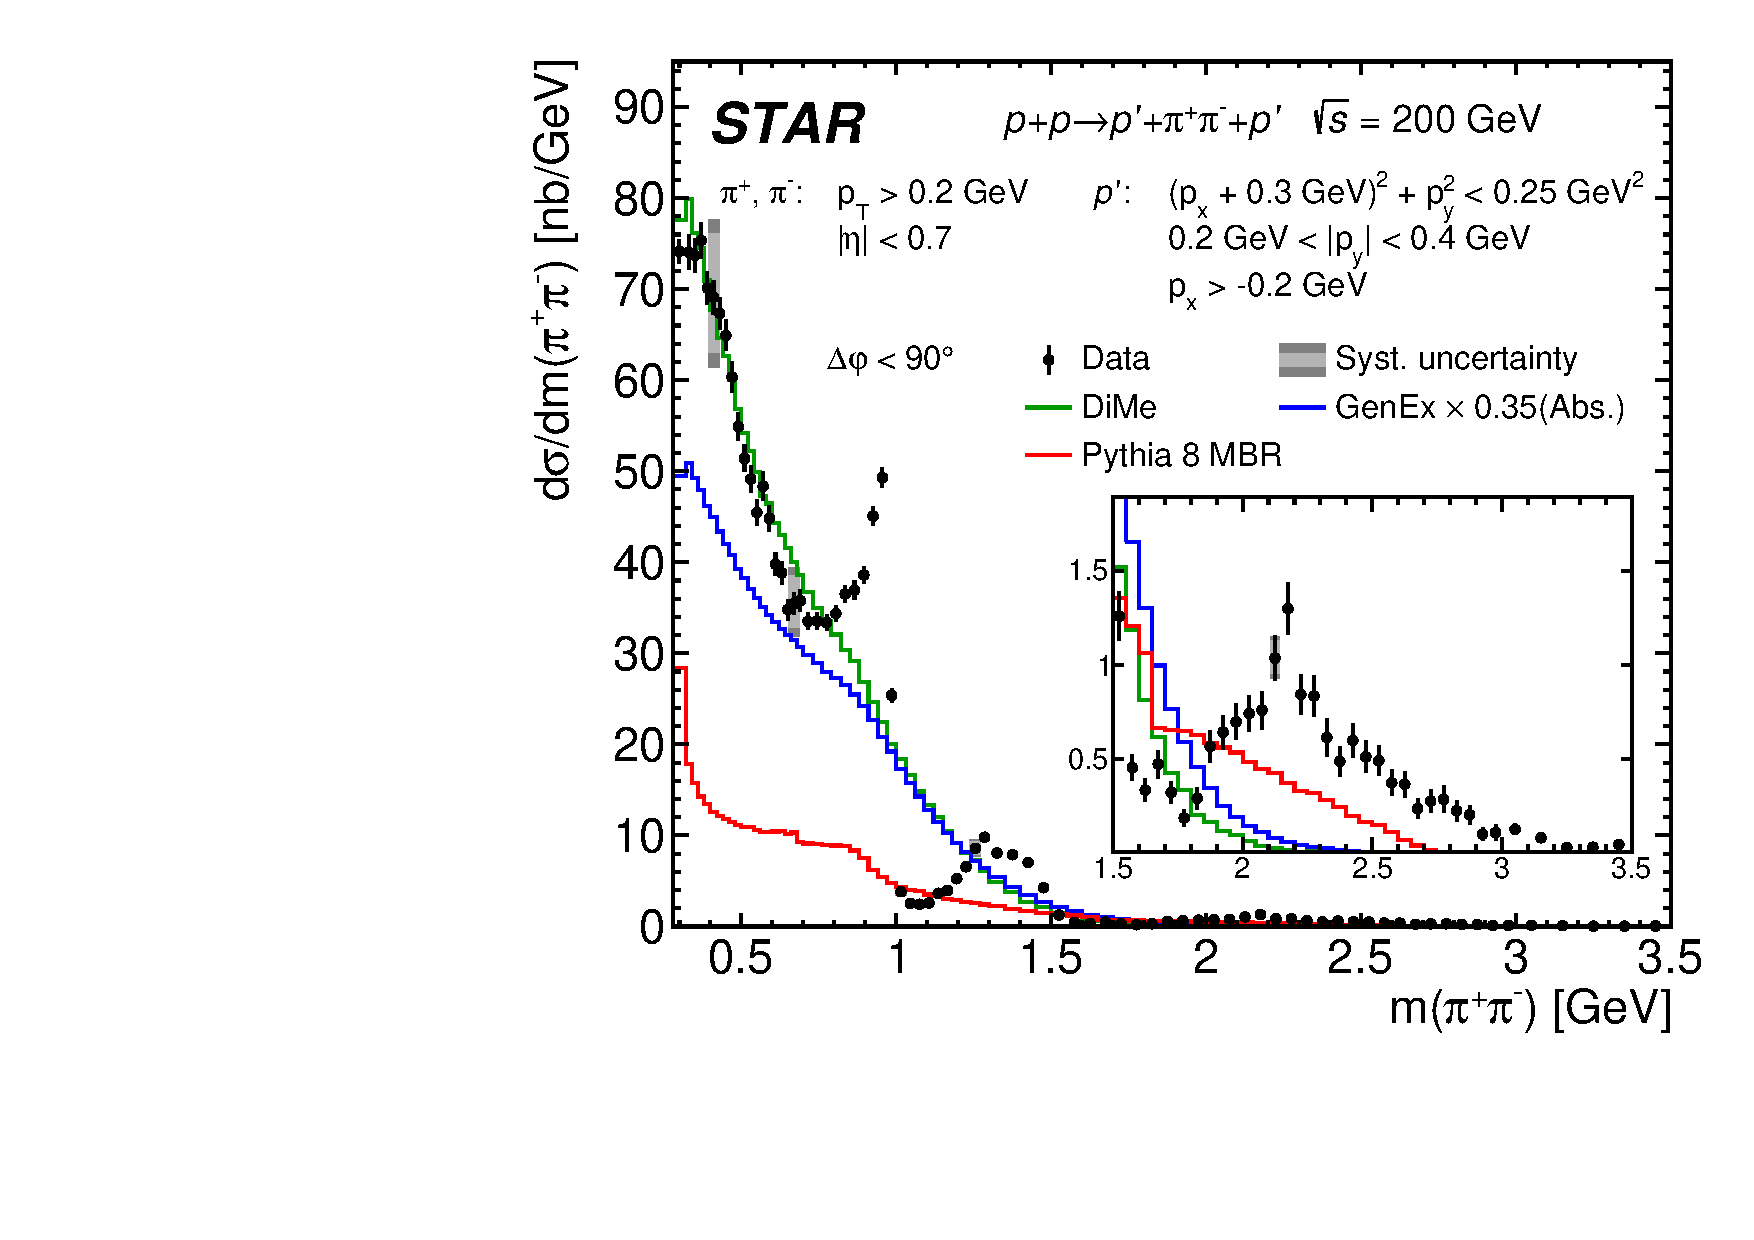
\includegraphics[width=.46\textwidth,page=1]{graphics/physicsResults/FinalResult_InvMass_DeltaPhiBin1_pion.pdf}
\hfill
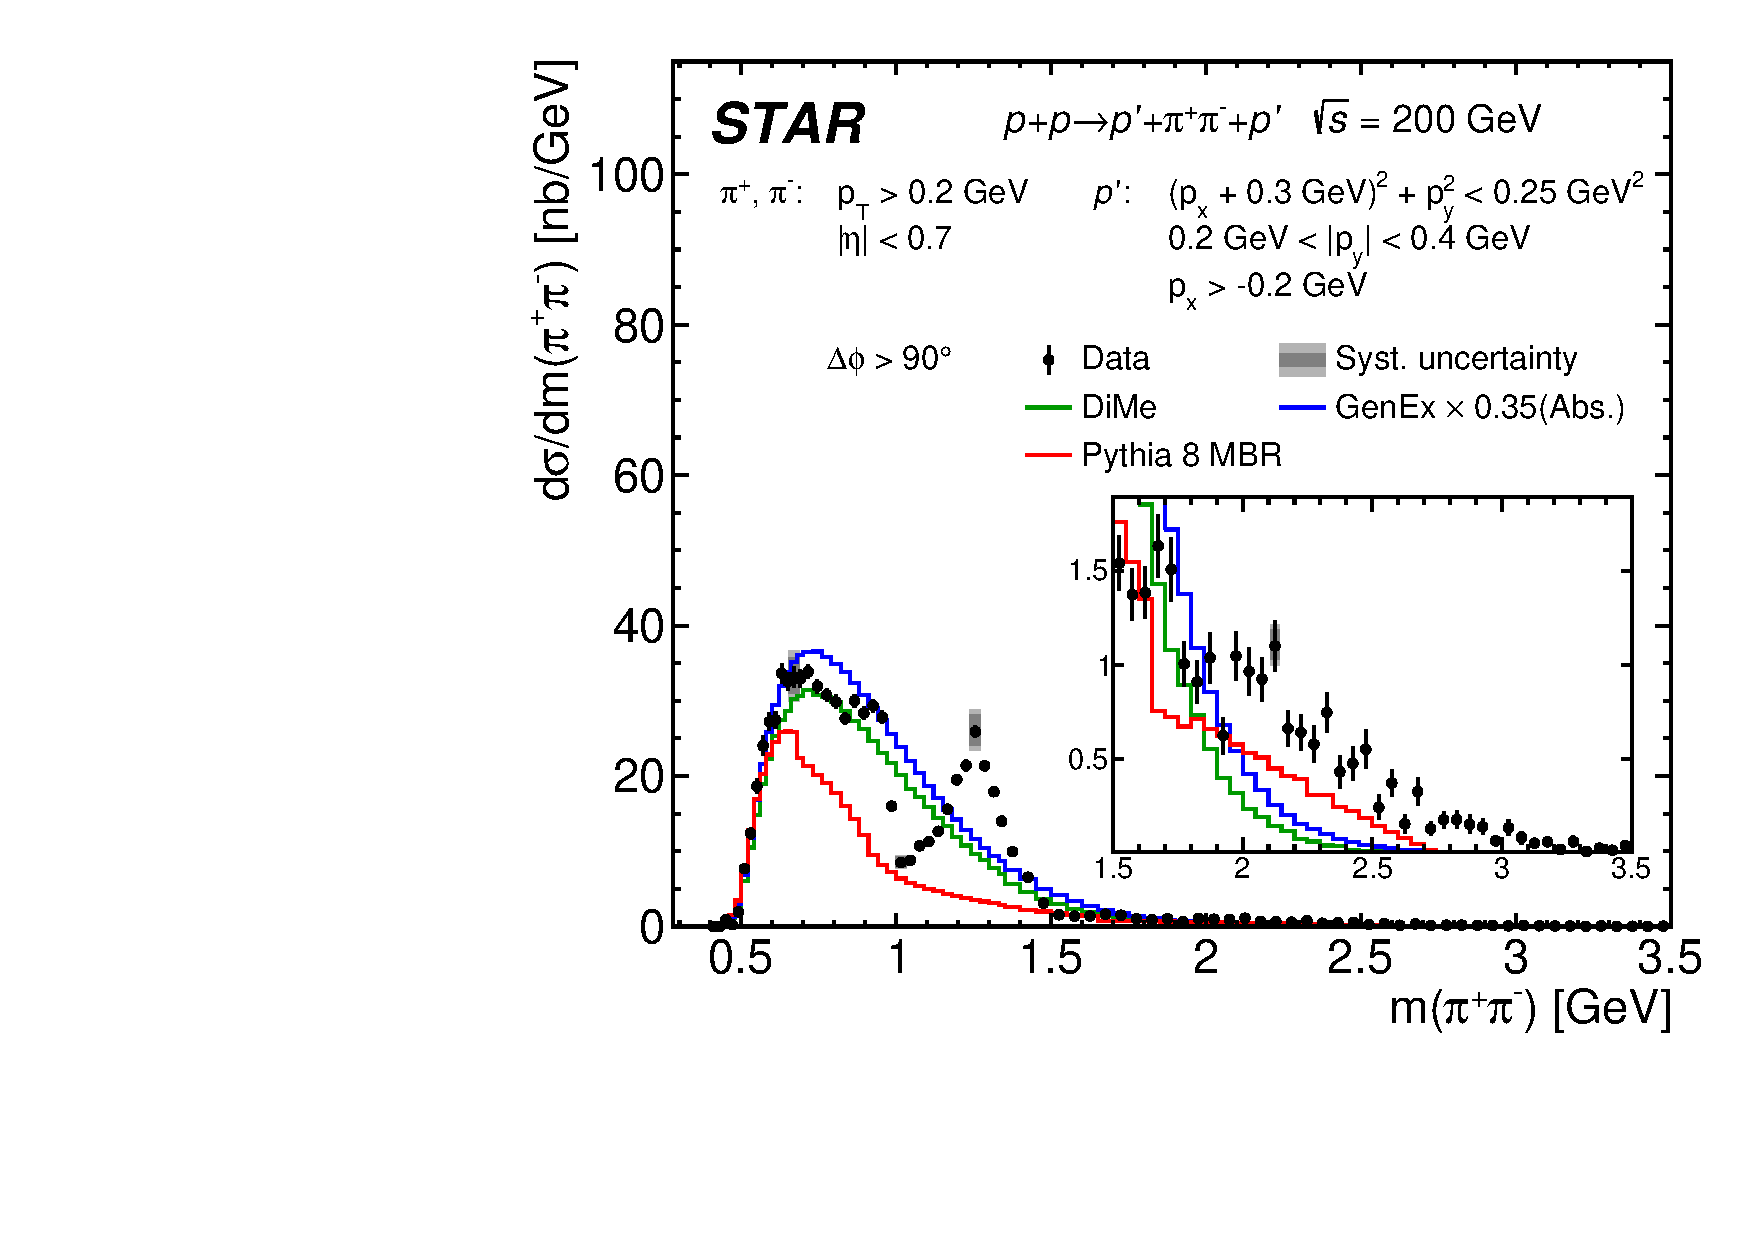
\includegraphics[width=.46\textwidth,page=1]{graphics/physicsResults/FinalResult_InvMass_DeltaPhiBin2_pion.pdf}
\hspace*{5pt}
\newline
\hspace*{5pt}
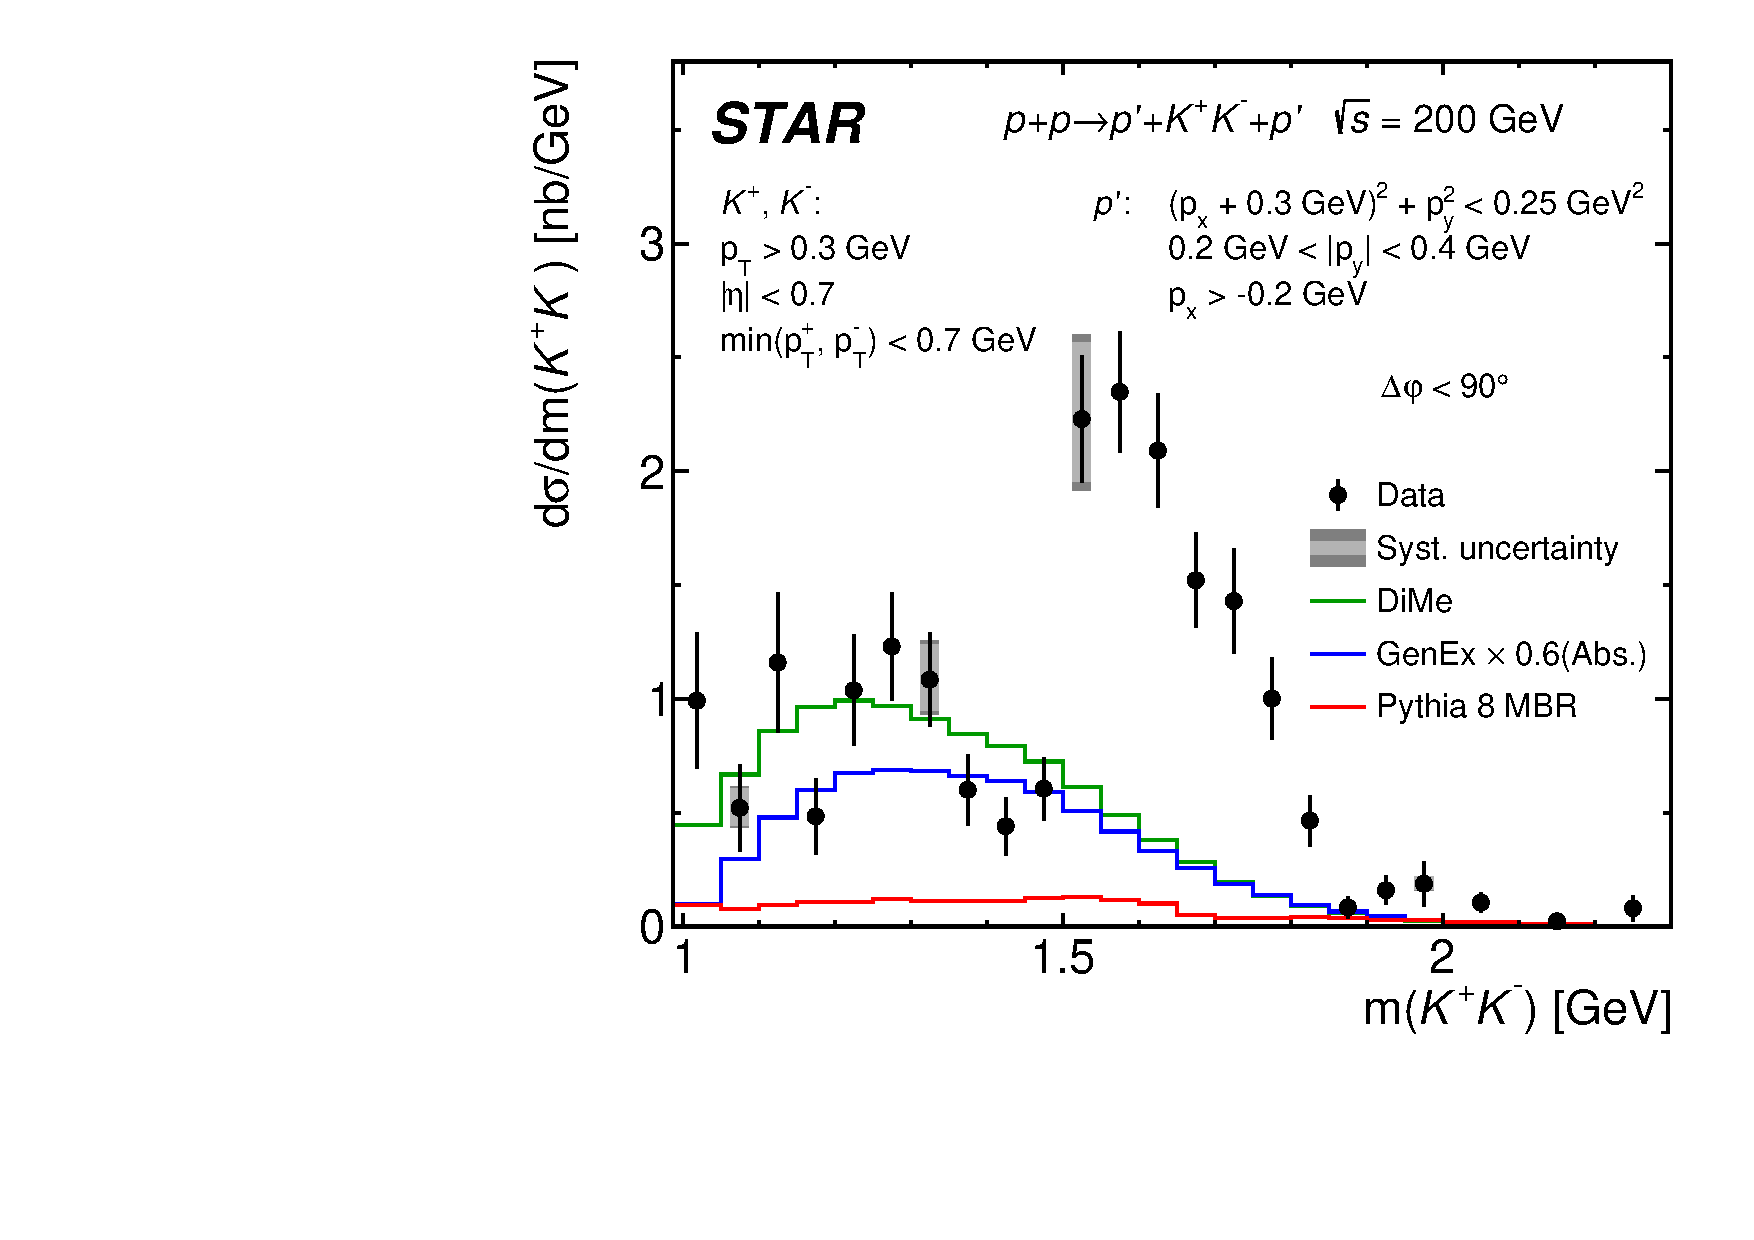
\includegraphics[width=.46\textwidth,page=1]{graphics/physicsResults/FinalResult_InvMass_DeltaPhiBin1_kaon.pdf}
\hfill
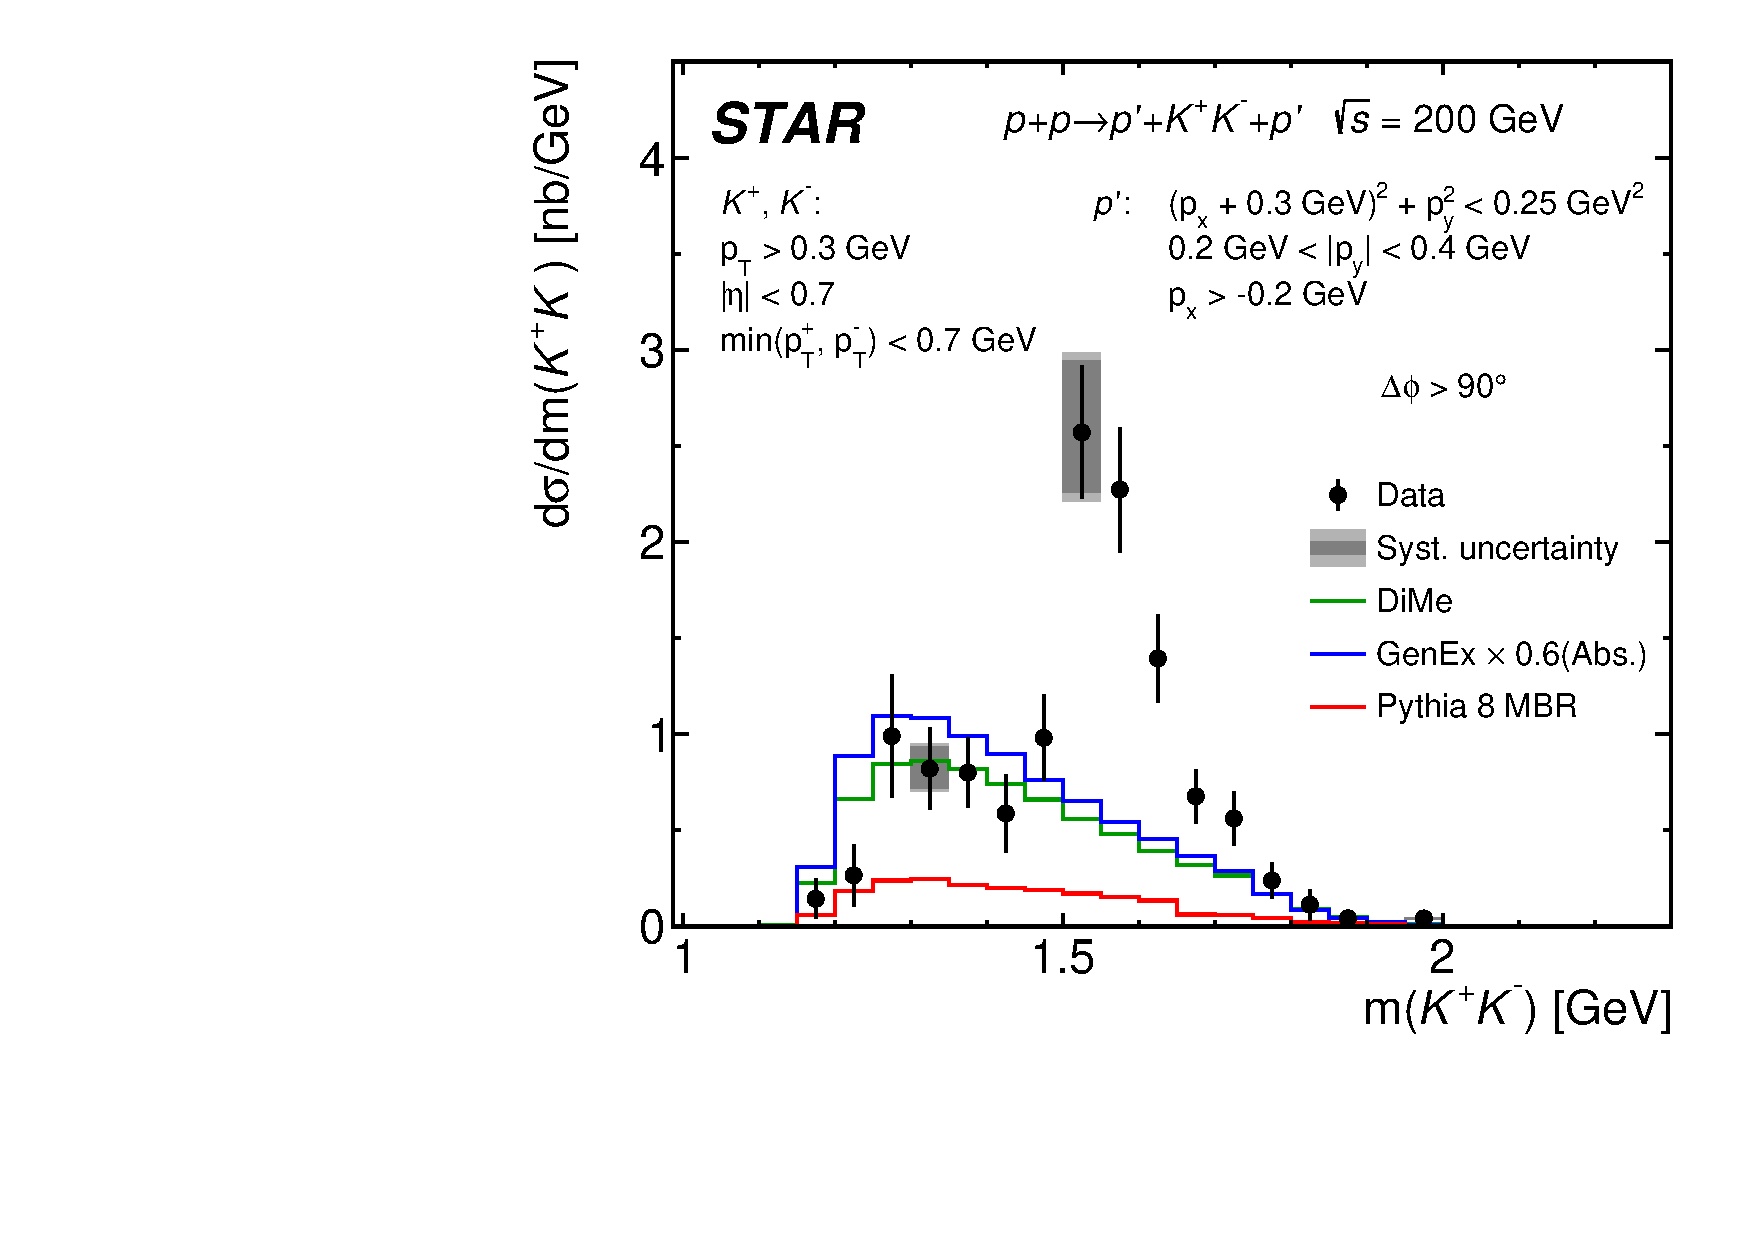
\includegraphics[width=.46\textwidth,page=1]{graphics/physicsResults/FinalResult_InvMass_DeltaPhiBin2_kaon.pdf}
\hspace*{5pt}
\newline
\hspace*{5pt}
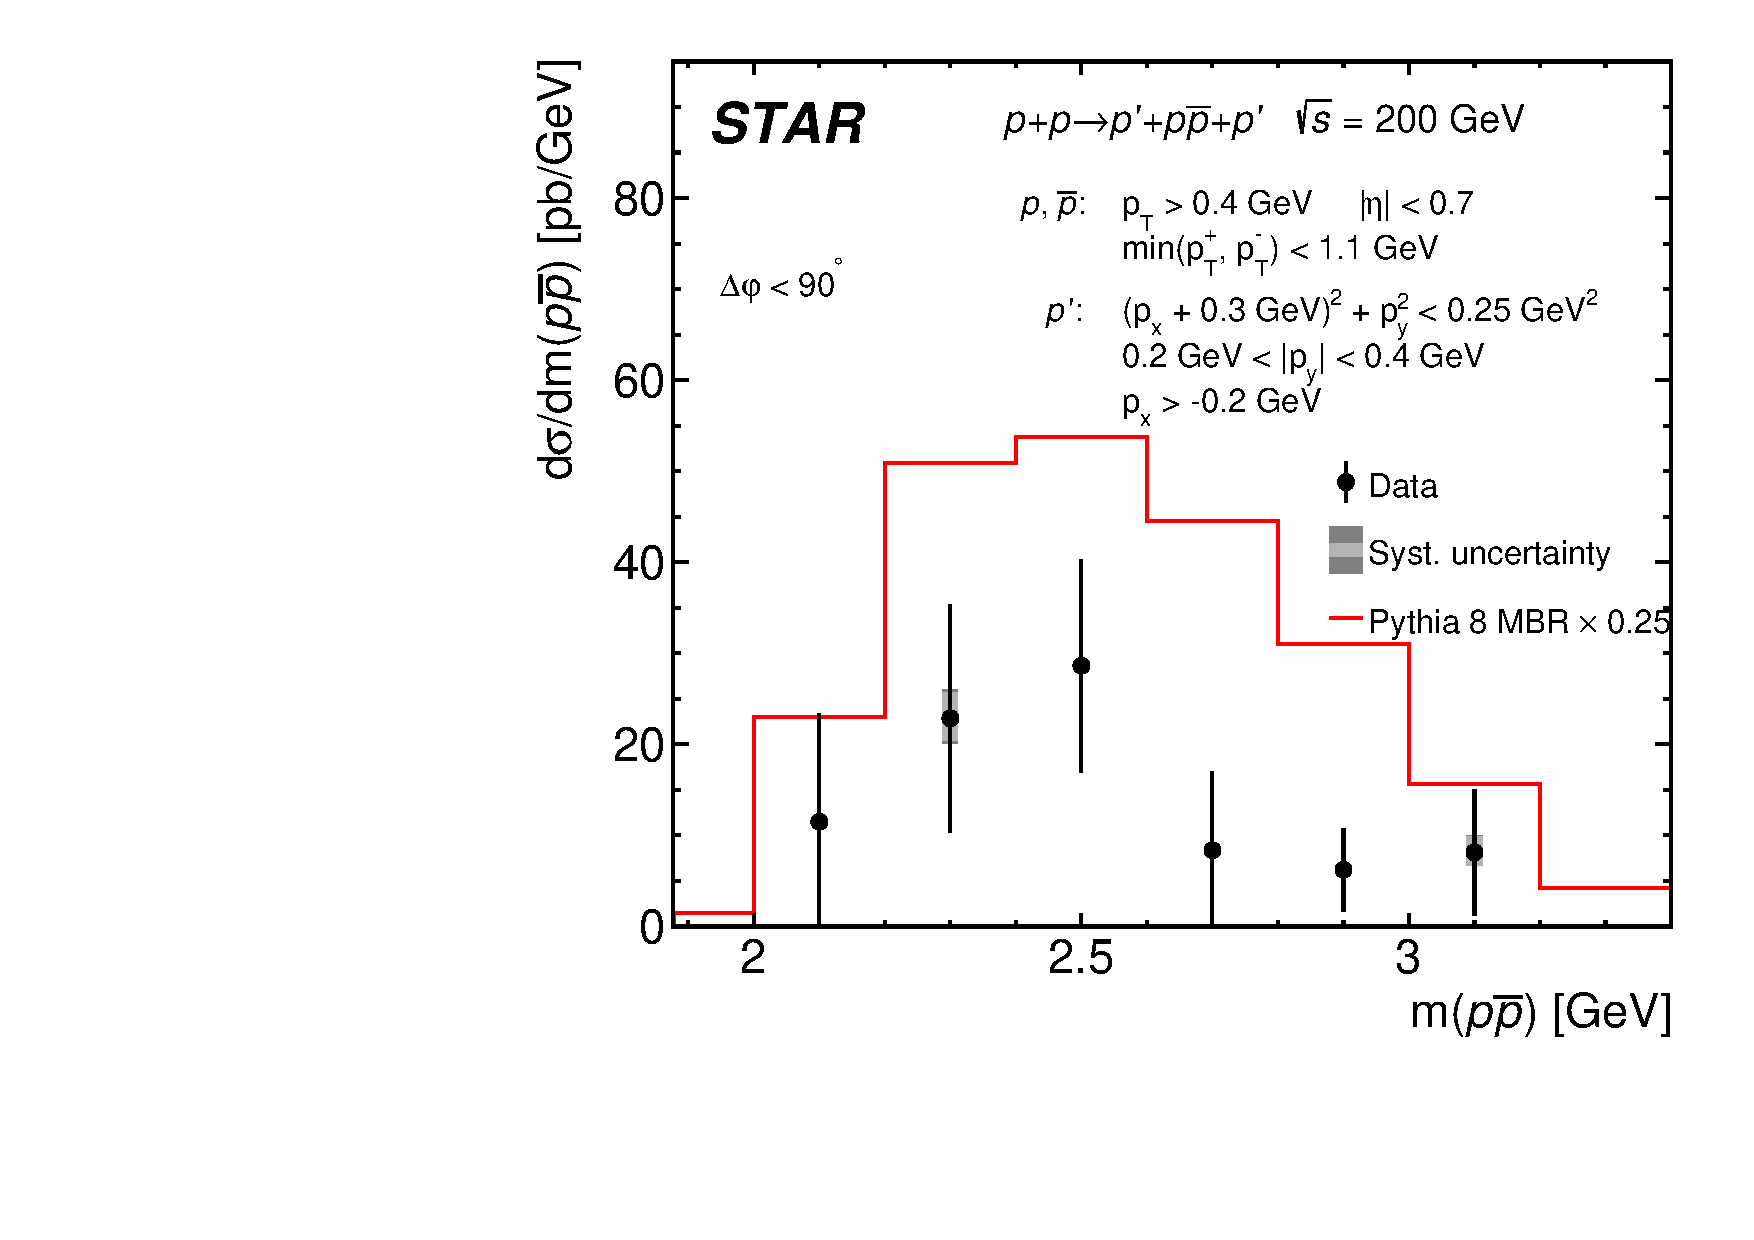
\includegraphics[width=.46\textwidth,page=1]{graphics/physicsResults/FinalResult_InvMass_DeltaPhiBin1_proton.pdf}
\hfill
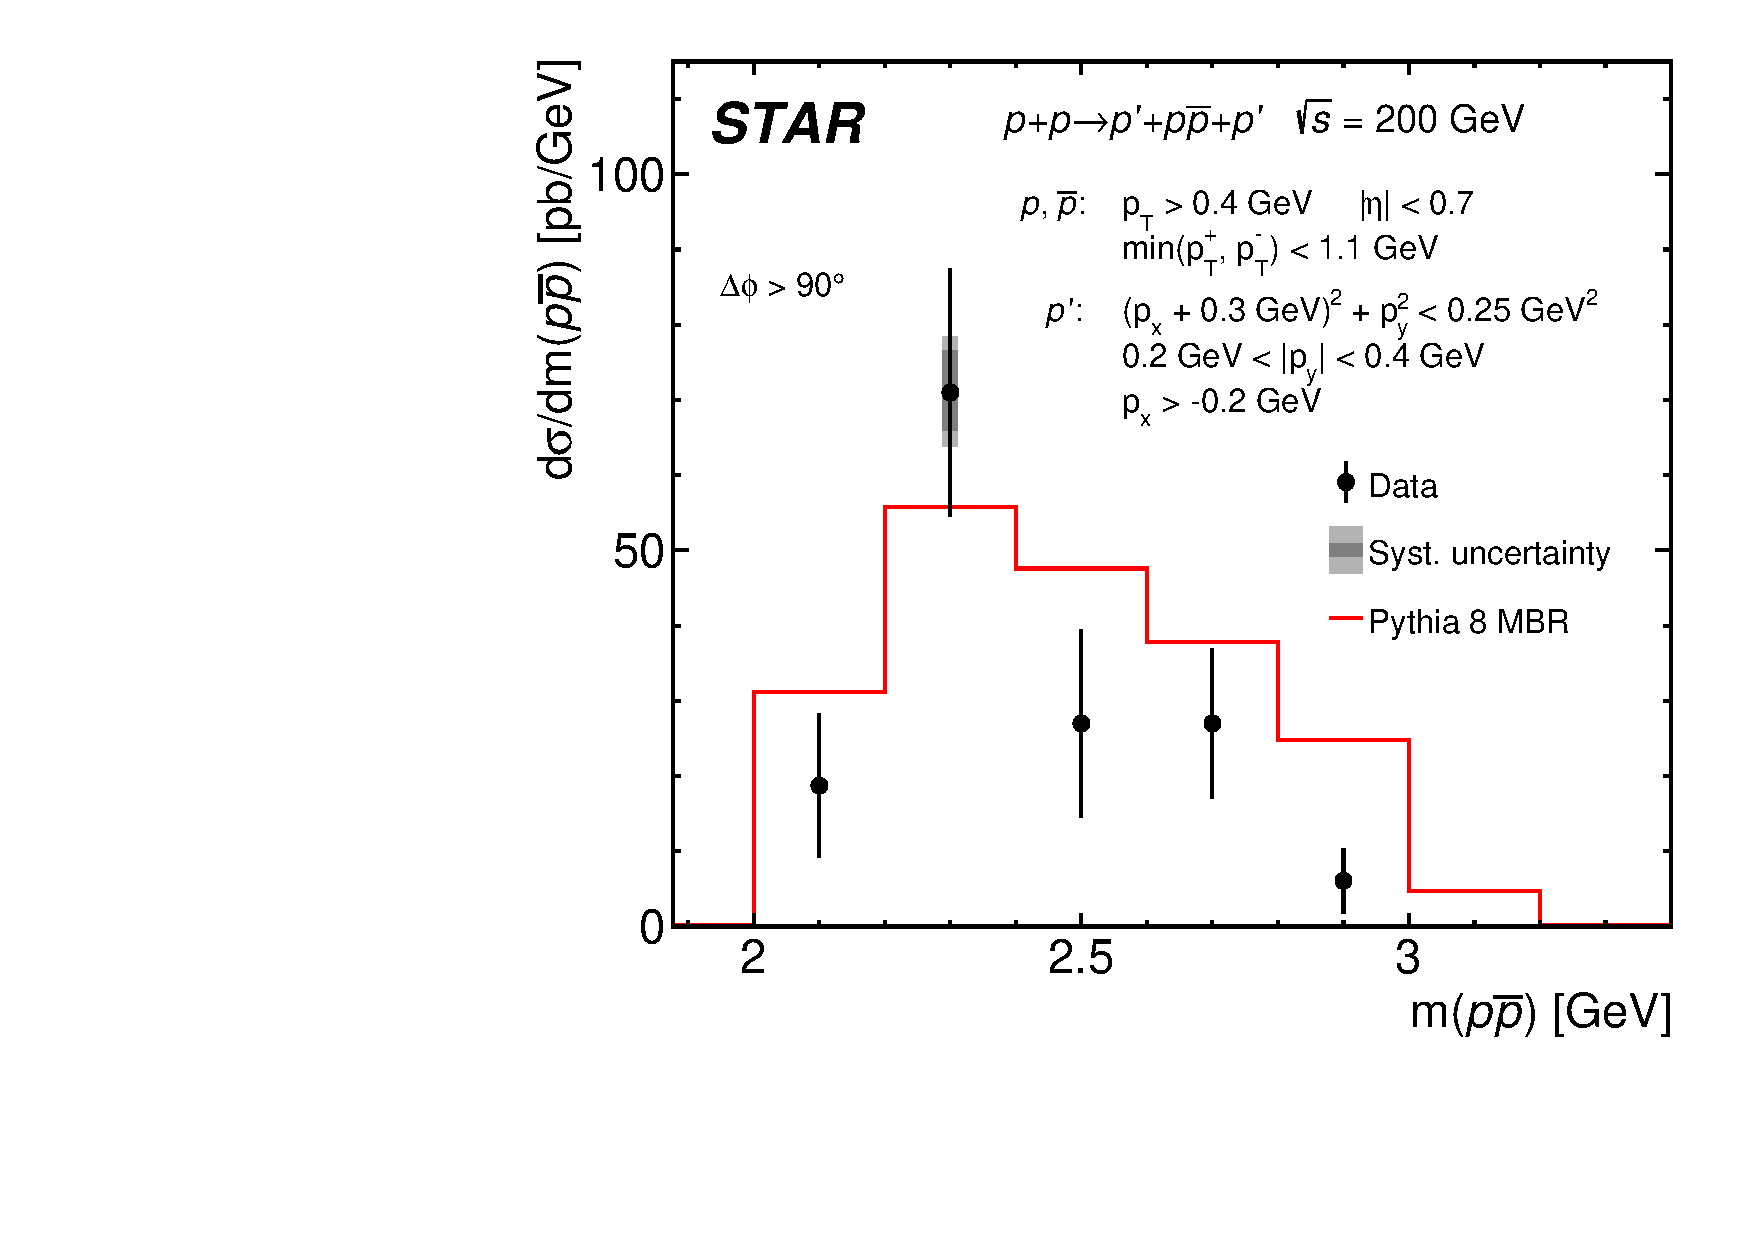
\includegraphics[width=.46\textwidth,page=1]{graphics/physicsResults/FinalResult_InvMass_DeltaPhiBin2_proton.pdf}
\hspace*{5pt}
%
\caption{Differential cross sections for CEP of charged particle pairs $\pi^+\pi^-$ (top), $K^+K^-$ (middle) and $p\bar{p}$ (bottom) as a function of the invariant mass of the pair in two $\Delta\phi$ regions: $\Delta\phi<90$ degree (left column) and $\Delta\phi>90$ degree (right column) measured in the fiducial region explained on the plots. Data are shown as solid points with error bars representing the statistical uncertainties. The typical systematic uncertainties are shown as gray boxes for only few data points as they are almost fully correlated between neighboring bins. Predictions from MC models GenEx, DiMe and MBR are shown as histograms.}
\label{results_3}
\end{figure}

{
\renewcommand{\arraystretch}{1.5}
\begin{table}[]\centering
\begin{tabular}{cc|T{1.4cm}T{1.4cm}T{1.4cm}|T{1.4cm}T{1.4cm}T{1.4cm}}
\multicolumn{2}{c|}{~}   & \multicolumn{3}{c|}{$\bm{\Delta\varphi<90^{\circ}}$} &  \multicolumn{3}{c}{$\bm{\Delta\varphi>90^{\circ}}$}  \\
    \multicolumn{2}{c|}{~}  & \multicolumn{1}{c}{$\bm{\pi^{+}\pi^{-}}$} & \multicolumn{1}{c}{$\bm{K^{+}K^{-}}$} & \multicolumn{1}{c|}{$\bm{p\bar{p}}$} & \multicolumn{1}{c}{$\bm{\pi^{+}\pi^{-}}$} & \multicolumn{1}{c}{$\bm{K^{+}K^{-}}$} & \multicolumn{1}{c}{$\bm{p\bar{p}}$} \\ \hline
\multicolumn{2}{c|}{$\bm{ \sigma_{\text{\bf{fid}}} }$} & $38.1$~nb & $976$~pb& $17.7$~pb & $18.4$~nb & $533$~pb & $31.5$~pb \\ %\hline
\multicolumn{2}{c|}{$\bm{ \delta_{\text{\bf{stat}}} }$} & $0.2$~nb & $46$~pb& $3.6$~pb & $0.1$~nb & $33$~pb & $5.4$~pb \\ %\hline
\multicolumn{2}{c|}{$\bm{ \delta_{\text{\bf{syst}}} }$} & $^{\hphantom{+}4.3}_{-4.0}$~nb & $^{\hphantom{+}156}_{-140}$~pb & $^{\hphantom{+}2.3}_{-2.1}$~pb & $^{\hphantom{+}2.0}_{-1.8}$~nb & $^{\hphantom{+}84}_{-76}$~pb & $^{\hphantom{+}3.9}_{-3.6}$~pb \\ \hline
\multirow{6}{*}{  \specialcell{ $\bm{ \frac{\delta_{\text{\bf{syst}}}}{\sigma_{\text{\bf{fid}}}} }$ \\ $\bm{[\text{\bf{\%}}]}$ }   }   &  Total & $\prescript{11.4}{-10.5}{~~~}$ & $\prescript{16.0}{-14.3}{~~~}$ & $\prescript{13.0}{-11.8}{~~~}$ & $\prescript{10.7}{-10.0}{~~~}$ & $\prescript{15.8}{-14.2}{~~~}$ & $\prescript{12.4}{-11.6}{~~~}$  \\ \cline{2-8}
&  TOF & $\prescript{3.1}{-2.9}{~~~}$ & $\prescript{10.0}{-8.6}{~~~}$ & $\prescript{5.4}{-4.9}{~~~}$ & $\prescript{2.7}{-2.5}{~~~}$ & $\prescript{10.3}{-8.9}{~~~}$ & $\prescript{5.7}{-5.2}{~~~}$  \\
&  TPC  & $\prescript{3.3}{-3.1}{~~~}$ & $\prescript{6.6}{-6.1}{~~~}$ & $\prescript{3.6}{-3.4}{~~~}$ & $\prescript{3.2}{-3.1}{~~~}$ & $\prescript{6.3}{-5.8}{~~~}$ & $\prescript{3.6}{-3.5}{~~~}$ \\
&  RP  &  $\prescript{7.3}{-6.1}{~~~}$ & $\prescript{7.4}{-6.2}{~~~}$ & $\prescript{8.4}{-6.9}{~~~}$ & $\prescript{6.3}{-5.4}{~~~}$ & $\prescript{6.9}{-5.8}{~~~}$ & $\prescript{7.0}{-5.2}{~~~}$ \\
&  Other  & $\prescript{2.6}{-2.4}{~~~}$ & $\prescript{2.7}{-2.4}{~~~}$ & $\prescript{2.9}{-2.4}{~~~}$ & $\prescript{2.6}{-2.4}{~~~}$ & $\prescript{2.6}{-2.4}{~~~}$ & $\prescript{3.2}{-2.4}{~~~}$ \\
& Lumi. & \multicolumn{6}{c}{$7.0$} \\ \hline
\end{tabular}
\caption{Integrated fiducial cross sections for CEP of $\pi^{+}\pi^{-}$, $K^{+}K^{-}$ and $p\bar{p}$ pairs in two ranges of azimuthal angle difference $\Delta\varphi$ between forward scattered protons. Statistical and systematic uncertainties are provided for each cross section, with the latter decomposed in the last part of the table into major components. Single number in a cell indicates symmetric uncertainty, while positive and negative number denotes asymmetric uncertainty.}\label{tab:xSecSyst}
\end{table}
}

% %
% \FloatBarrier
% %
% Such correlation between resonances seen in mass spectrum and azimuthal angle between outgoing protons indicates factorization breaking between the two proton vertices. In the range $\Delta\phi<$ 90 degrees the DiMe model well describes both normalization and shape of mass spectrum at $m(\pi^+\pi^-)<$ 0.5 GeV.
% %
% In case of the cross section for CEP of $K^+K^-$ pairs the data do not show any significant asymmetry except possible widening
% of the peak at $f_2^\prime(1520)$ in the region $\Delta\phi<90$ degrees which may indicate an enhancement of additional resonances around 1.7~GeV in this configuration.
% %
% In case of the cross section for CEP of $p\bar{p}$ pairs data do not show any significant asymmetry except possible enhancement in the $2.2-2.4$ mass range for the $\Delta\phi>90$ degrees region.\\
% %
% \indent
% Due to high statistics of the two-pion sample it is possible to study the CEP of $\pi^+\pi^-$ pairs in more detail.
% Figure~\ref{results_4} shows the differential cross sections for CEP of $\pi^+\pi^-$ pairs as a function of the pair rapidity (left column), $\Delta\phi$ (middle column) and $|t_1+t_2|$ (right column) in three characteristic ranges of the invariant mass of the pair: $m(\pi^+\pi^-)<1.0$ GeV (mainly non-resonant production), $1.0< m(\pi^+\pi^-) <1.5$ GeV ($f_2(1270)$ mass range) and $m(\pi^+\pi^-)>1.5$ GeV (higher invariant masses).\\
% %
% \noindent
% Figure~\ref{results_4} shows the differential cross sections for CEP of different particle species pairs as a function of the pair rapidity (left column), of the difference of forward protons azimuthal angles (middle column) and of the sum of squares of the four-momenta transfers at the proton vertices (right column), for the three invariant mass ranges. In the case of the cross section $d\sigma/dy$ all models agree in shape with data in all three mass ranges except for the GenEx and DiMe predictions in the highest mass range where predictions is narrower.
% 
% Strong suppression of the fiducial cross section close to $90^\circ$ is due to the STAR RP acceptance while asymmetry $0^\circ$ vs. $180^\circ$ in the lowest mass region is due to the STAR TPC acceptance. $\Delta\phi$ distribution is sensitive to absorption  which are treated fully differentialy in DiMe generator and only on average in GenEx. This is consistent with generally better agreement between data and DiMe expectations except $f_2(1270)$ mass region. MBR model predicts symmetric $\Delta\phi$ distributions in all mass ranges which is not supported by the data.
% 
% The slope of the cross section as the function of $|t_1+t_2|$ is less steep in the $f_2(1270)$ mass region compared to other mass regions. In the low mass region the DiMe prediction has steeper slope compared to data.\\
%
\begin{figure}[h]
\centering
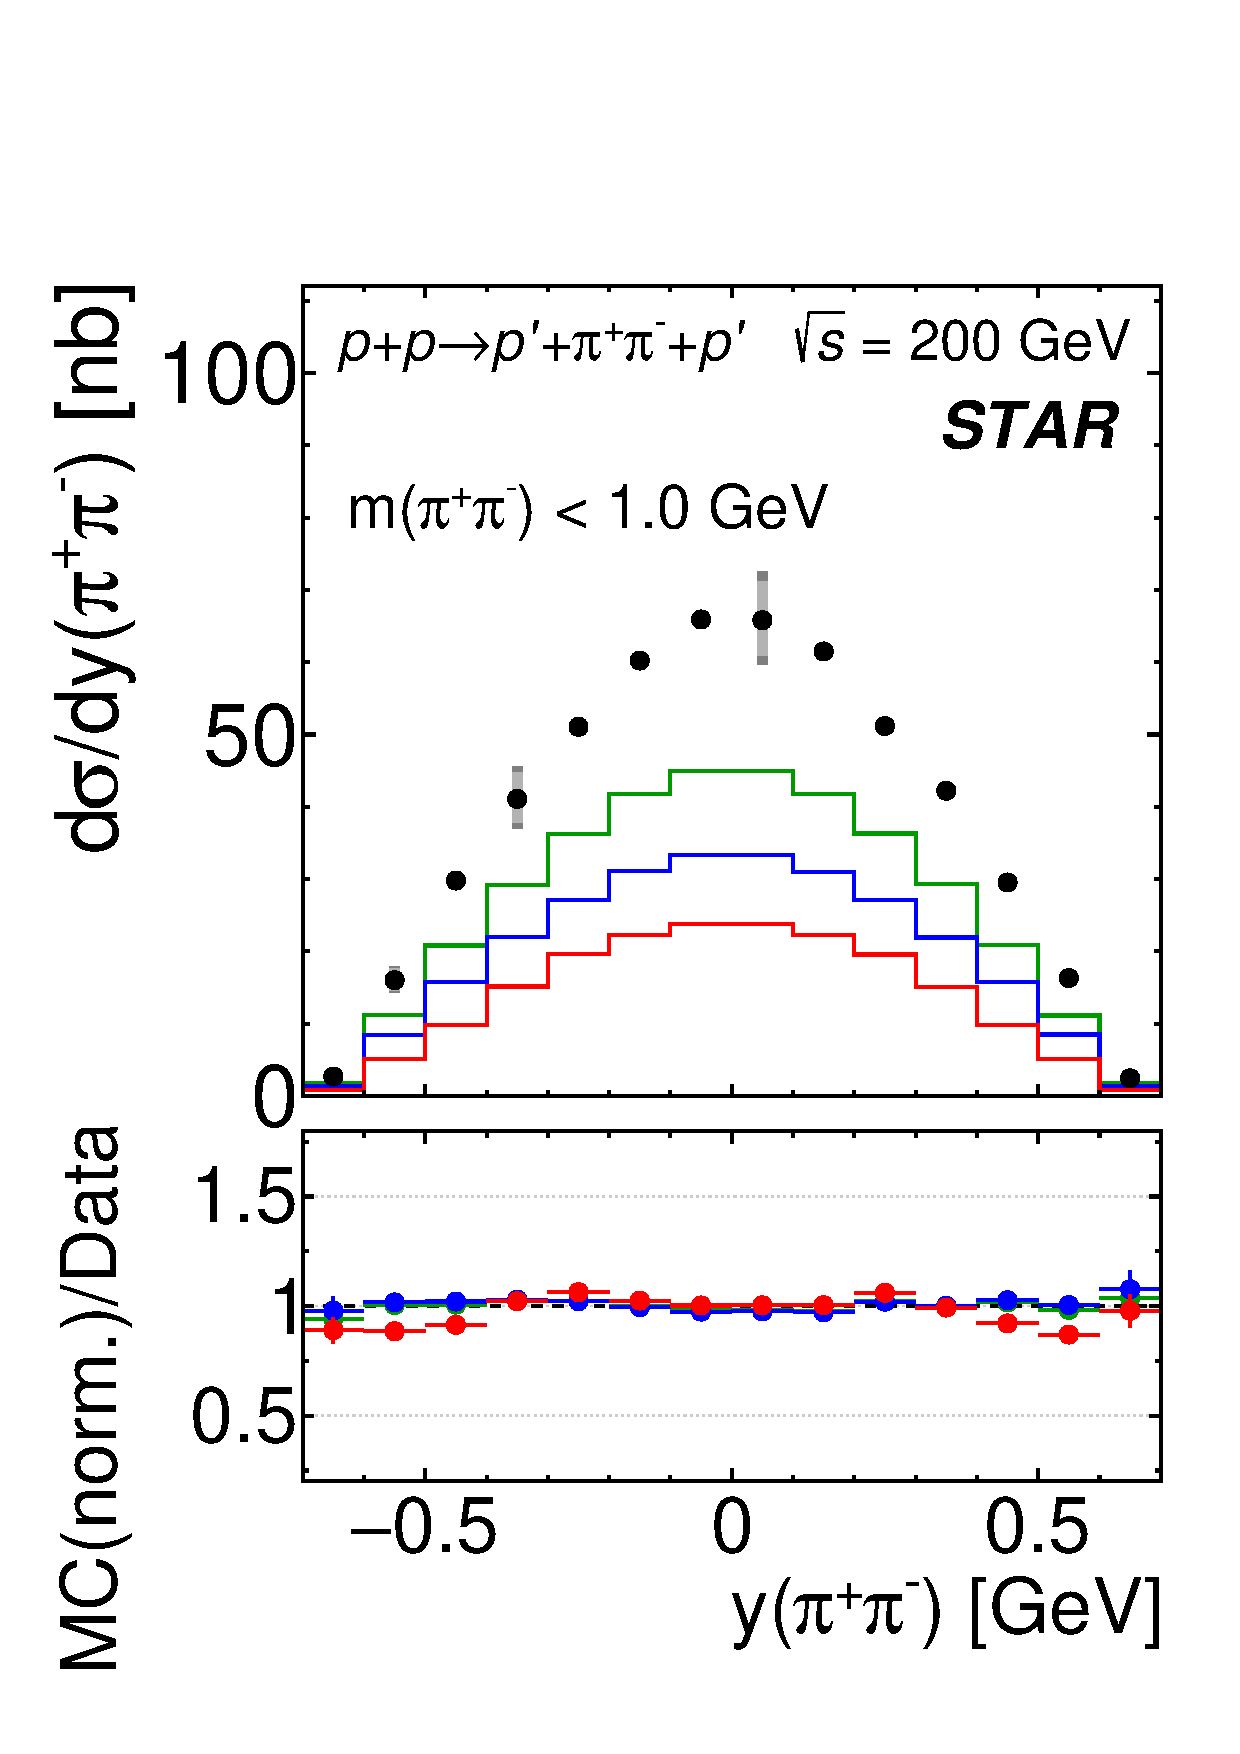
\includegraphics[width=.31\textwidth,page=1]{graphics/physicsResults/Ratio_FinalResult_Rapidity_pion_MassBin_1.pdf}
\hfill
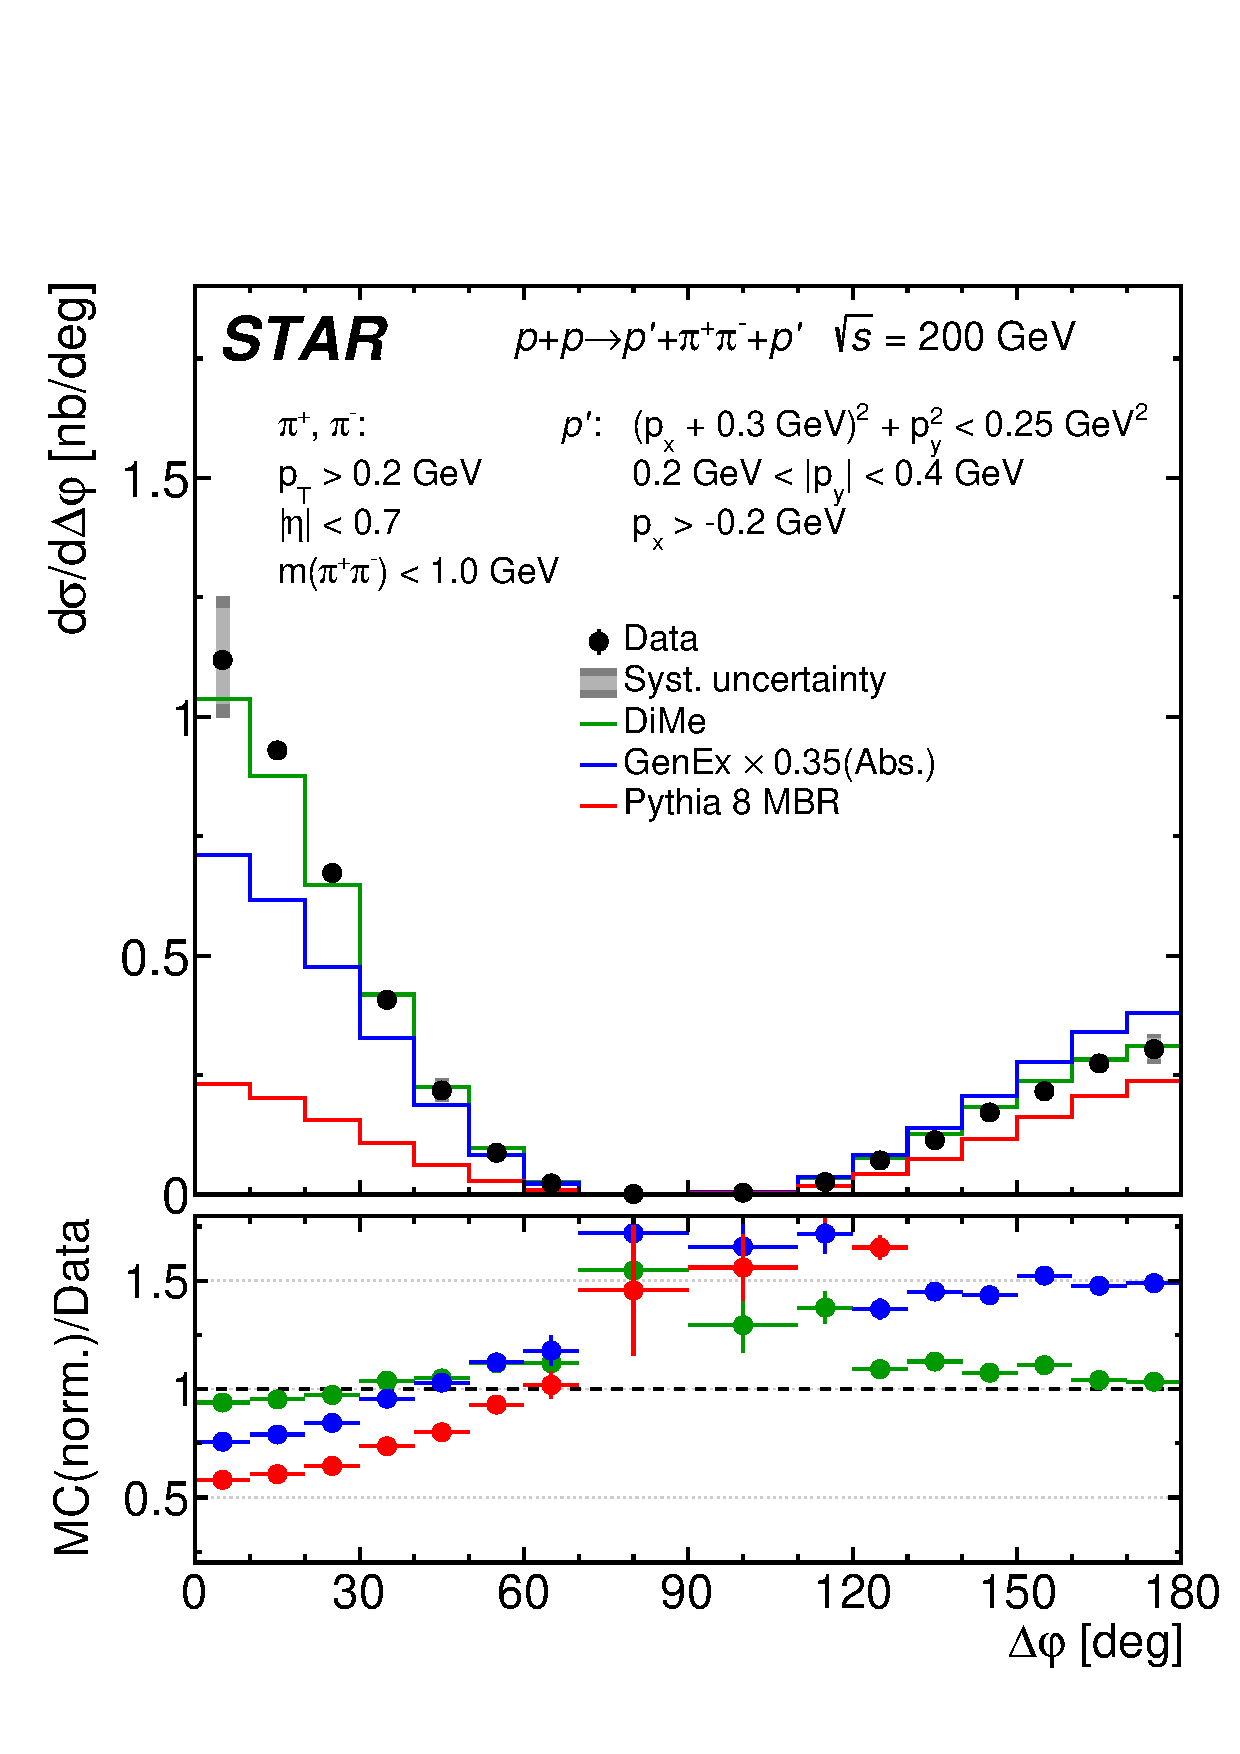
\includegraphics[width=.31\textwidth,page=1]{graphics/physicsResults/Ratio_FinalResult_DeltaPhi_pion_MassBin_1.pdf}
\hfill
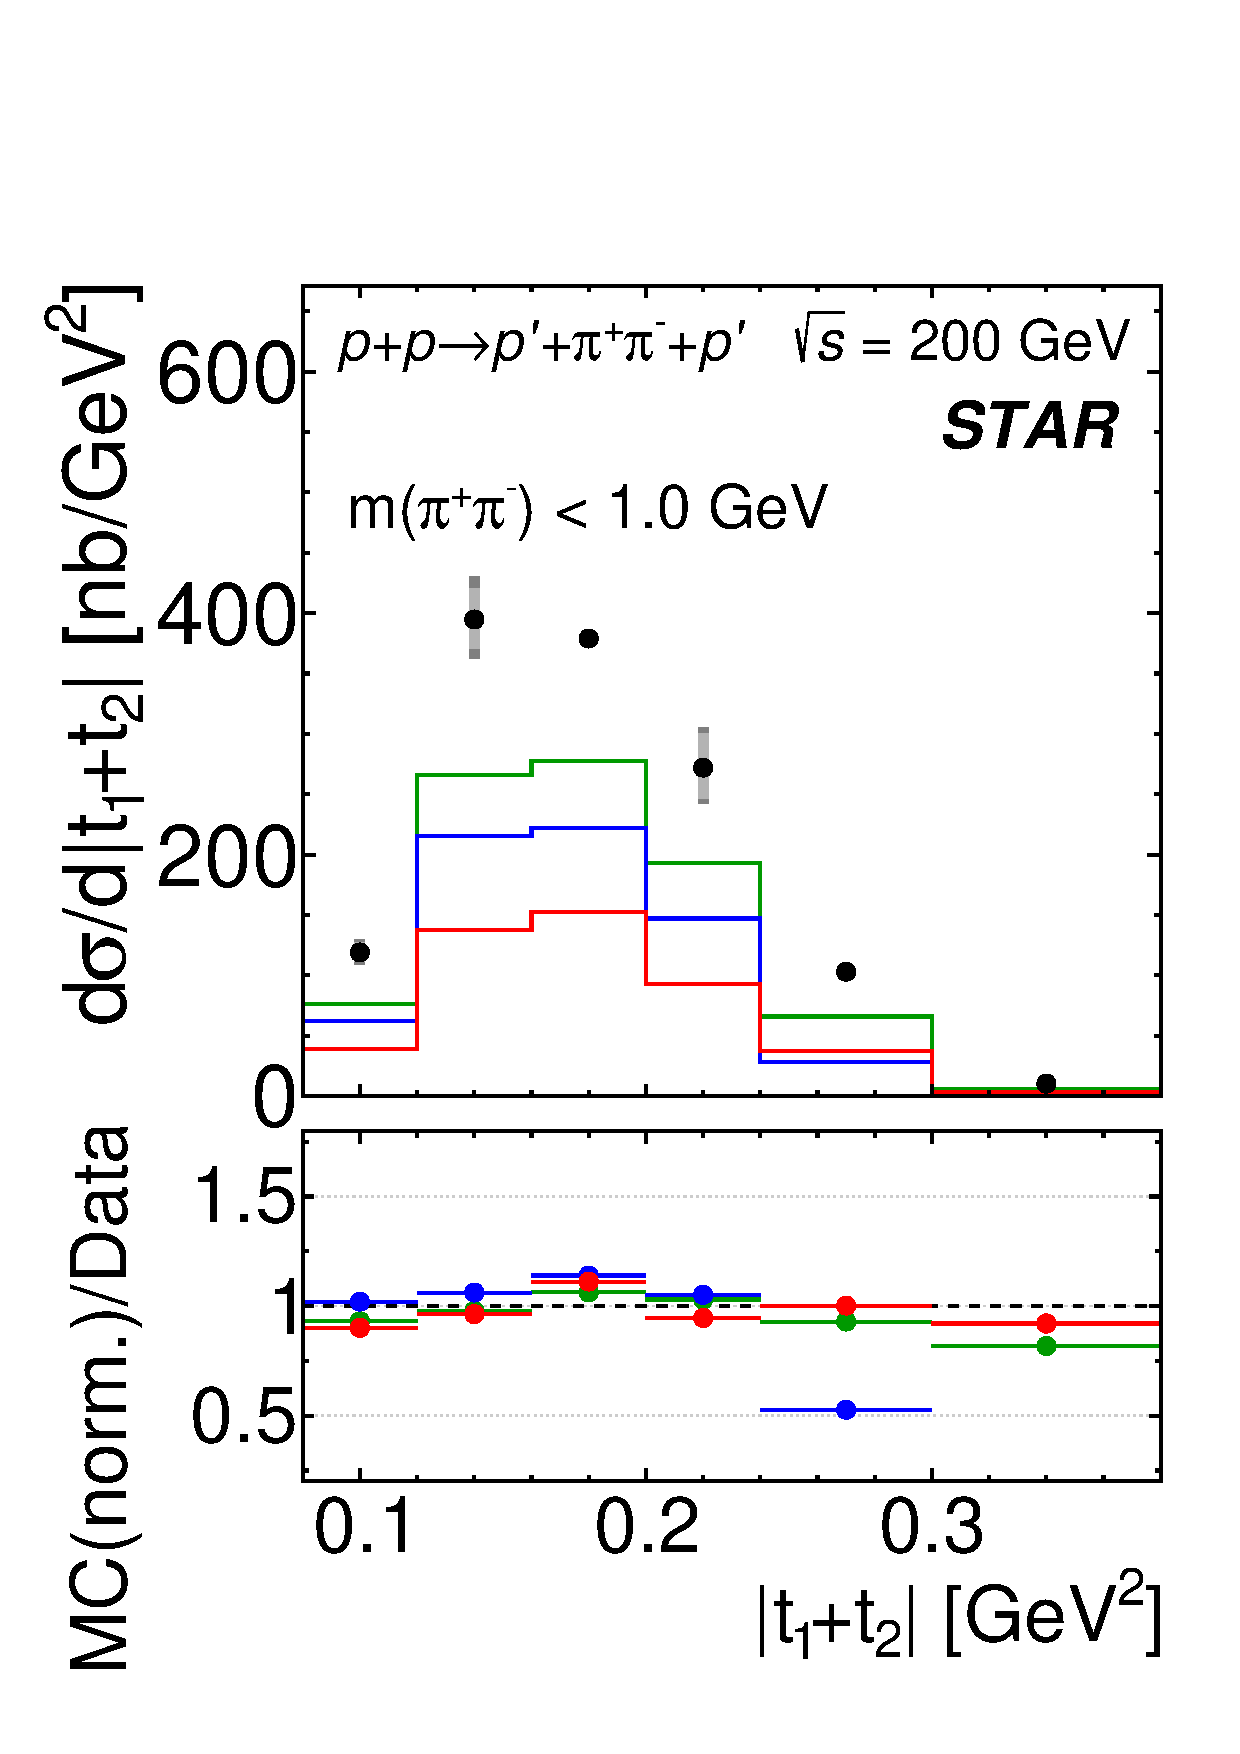
\includegraphics[width=.31\textwidth,page=1]{graphics/physicsResults/Ratio_FinalResult_MandelstamTSum_pion_MassBin_1.pdf}
\newline
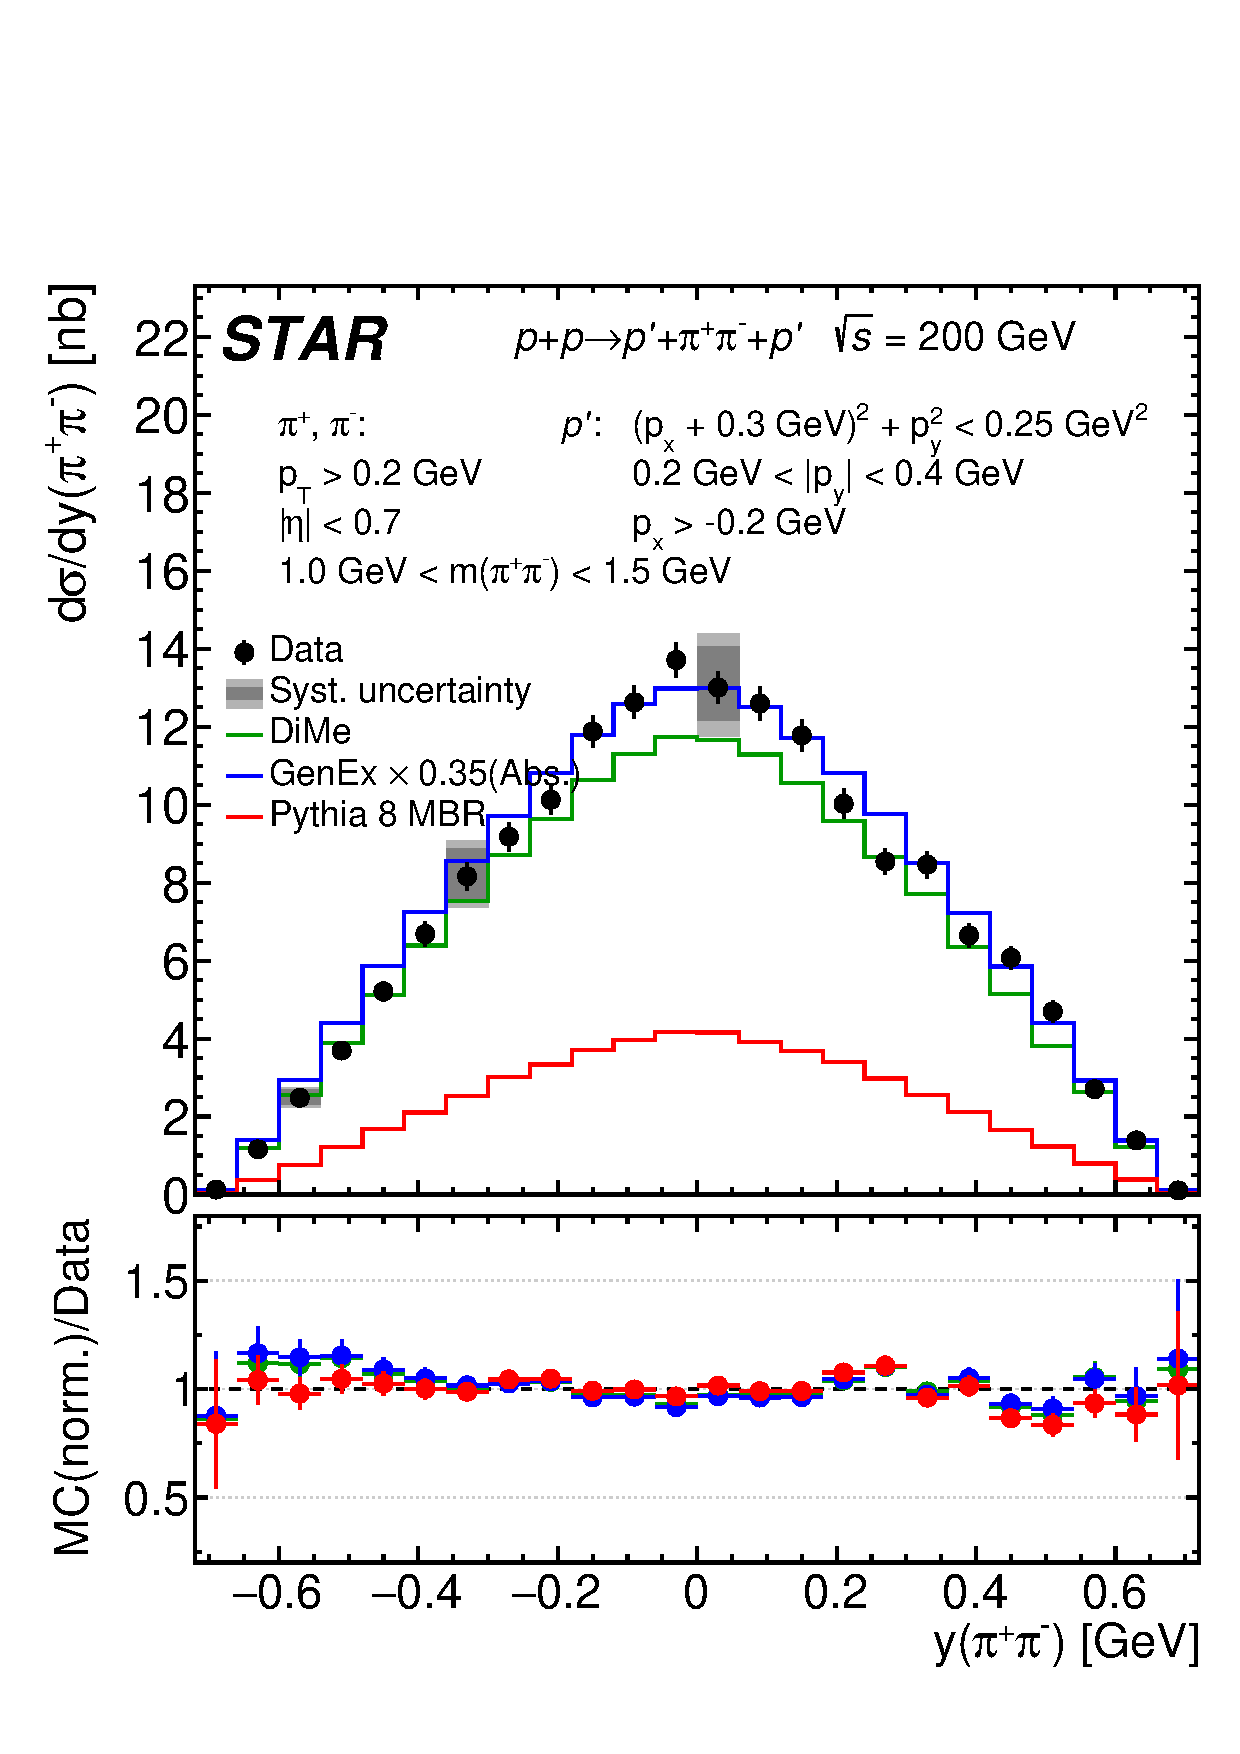
\includegraphics[width=.31\textwidth,page=1]{graphics/physicsResults/Ratio_FinalResult_Rapidity_pion_MassBin_2.pdf}
\hfill
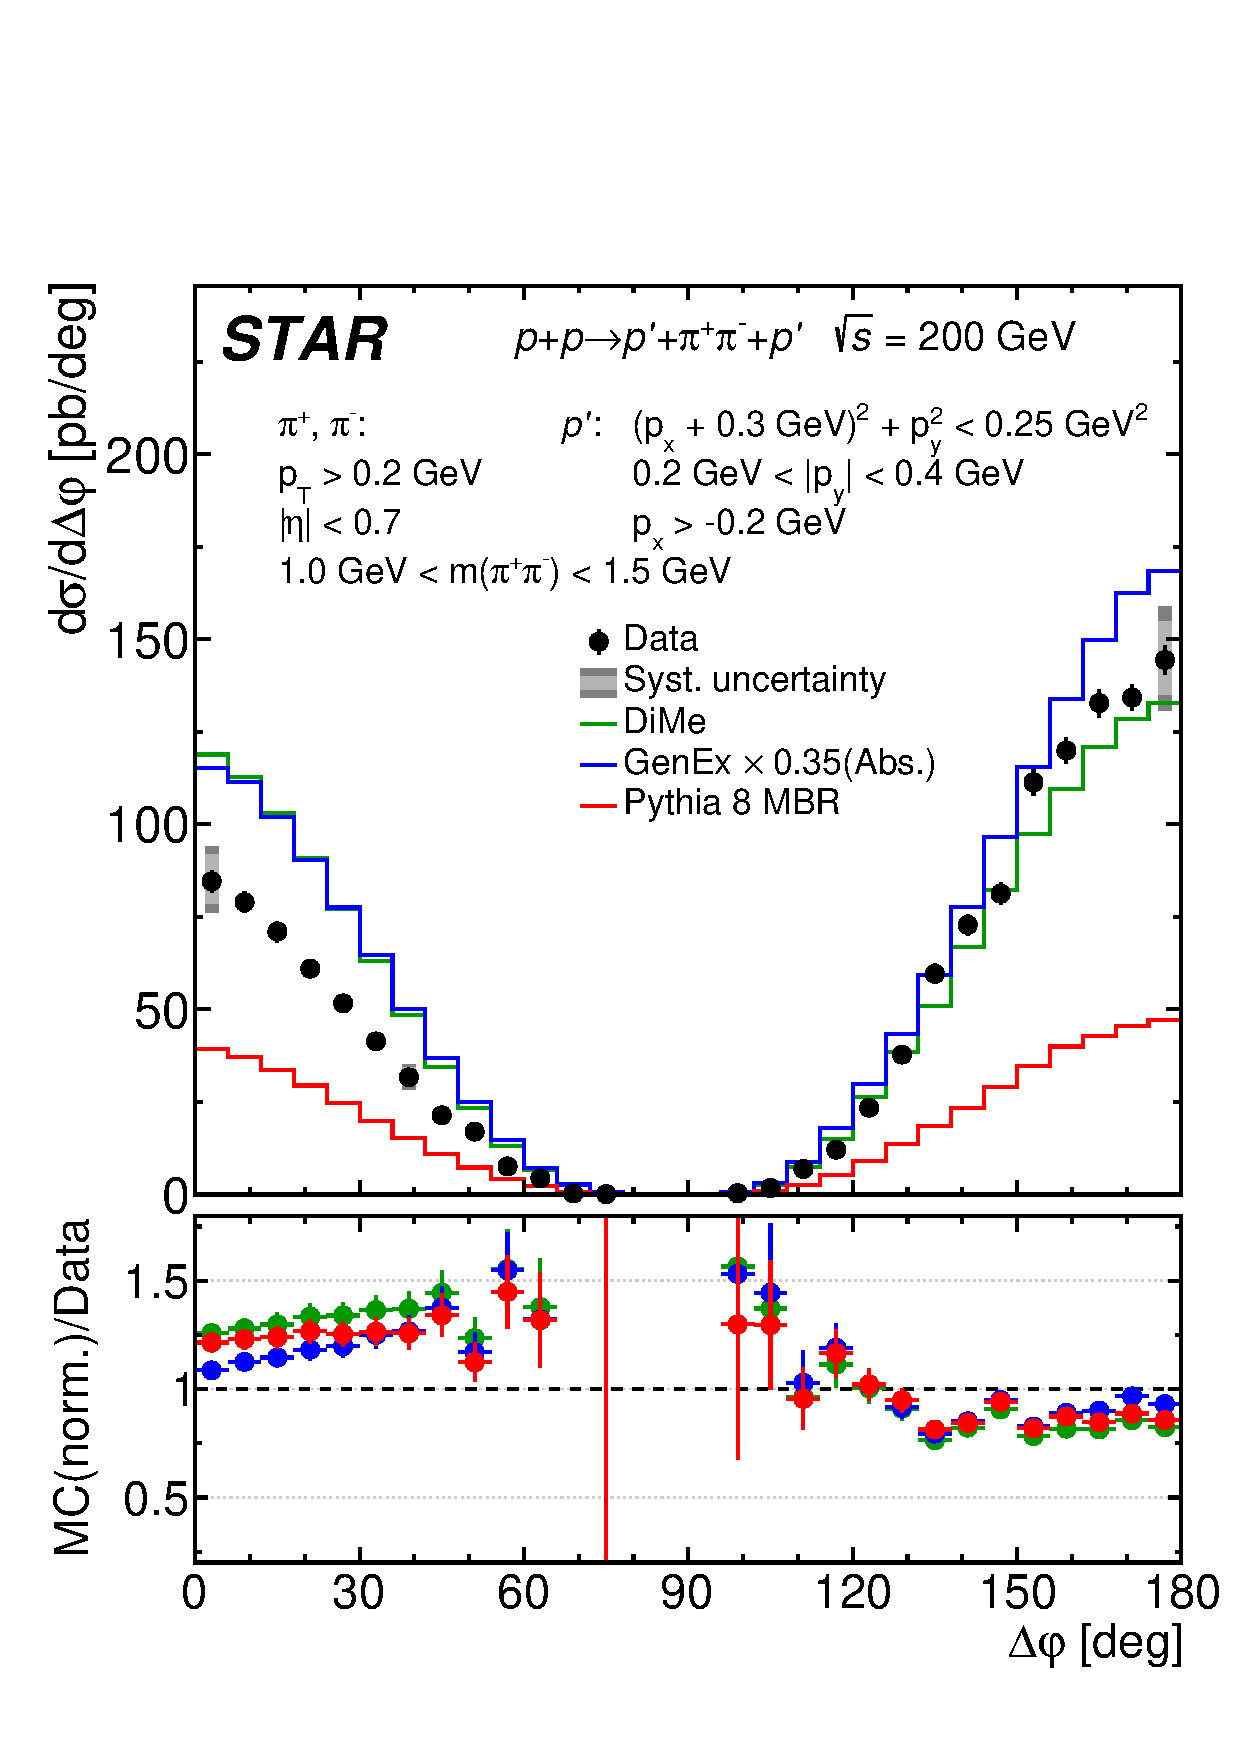
\includegraphics[width=.31\textwidth,page=1]{graphics/physicsResults/Ratio_FinalResult_DeltaPhi_pion_MassBin_2.pdf}
\hfill
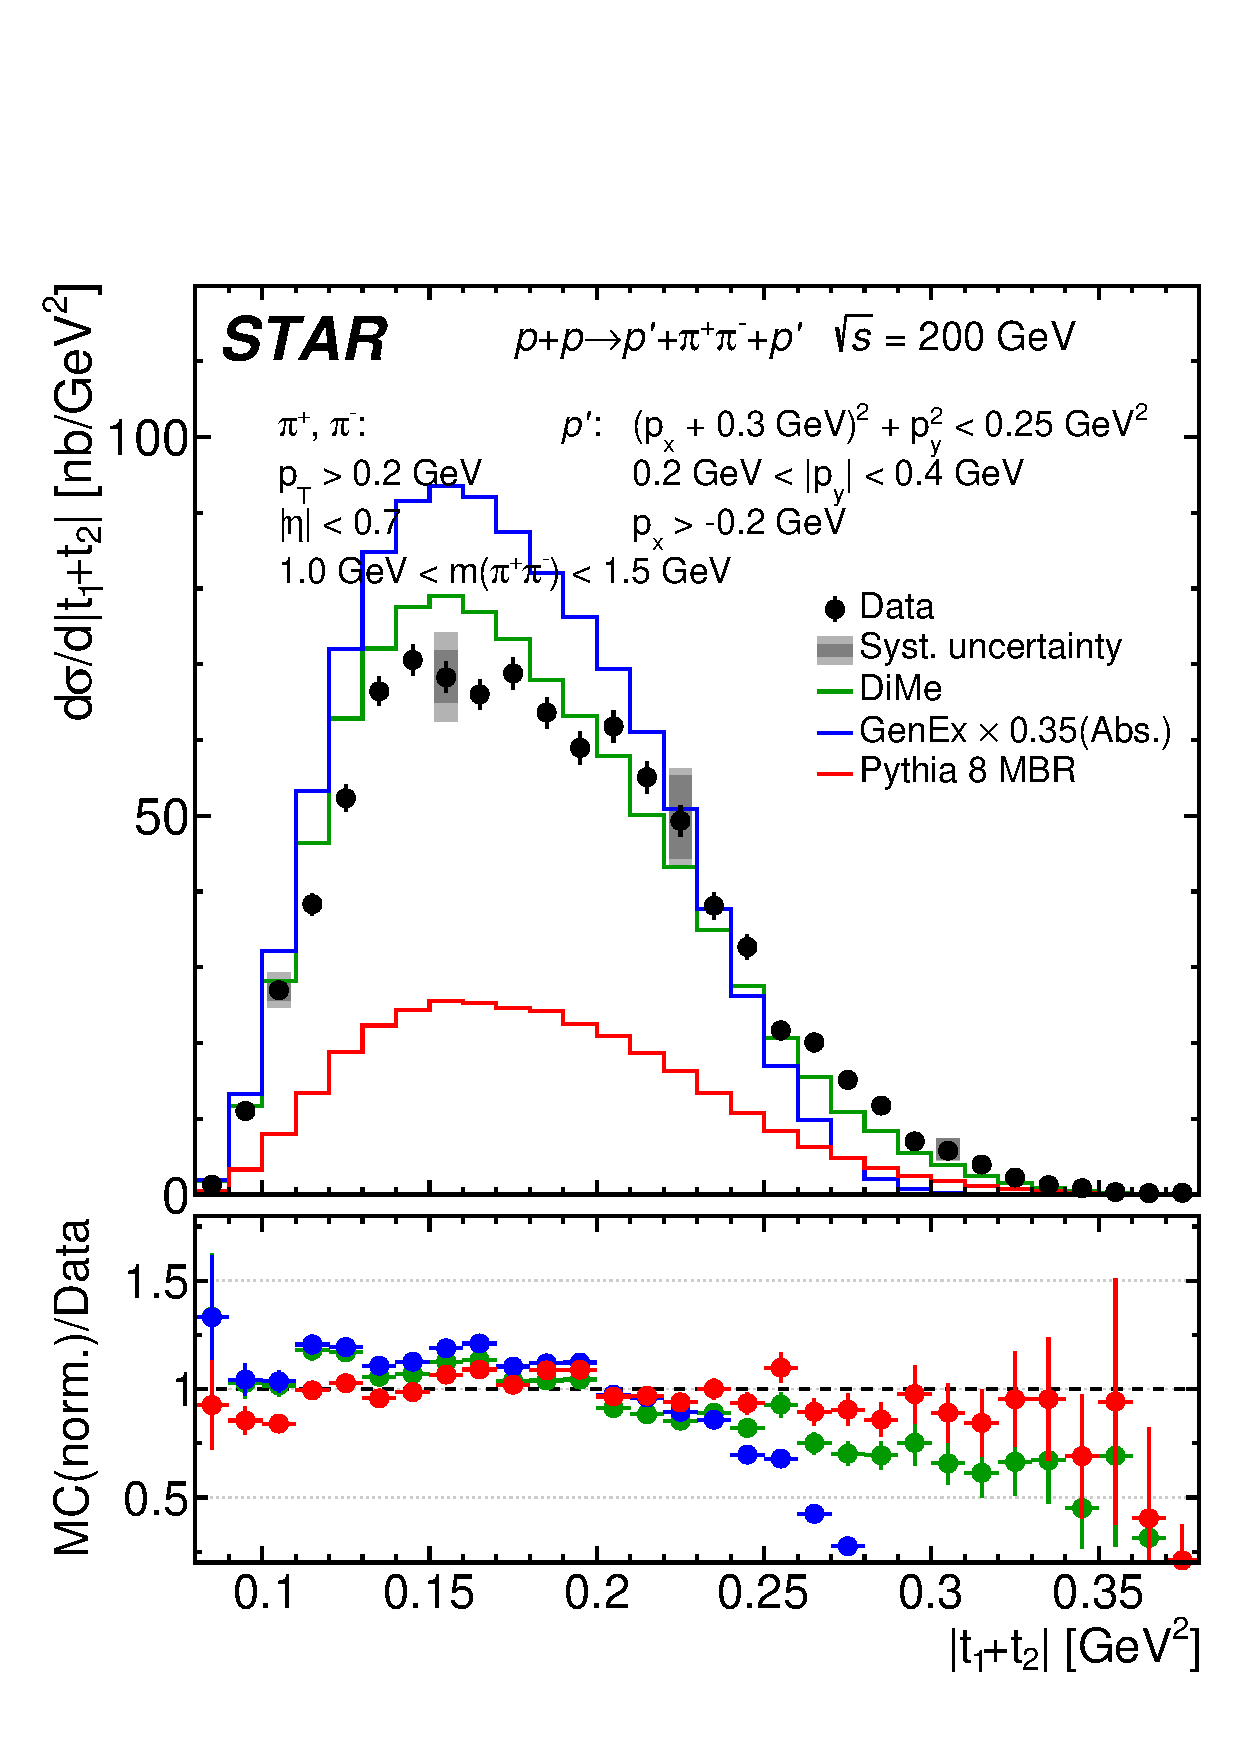
\includegraphics[width=.31\textwidth,page=1]{graphics/physicsResults/Ratio_FinalResult_MandelstamTSum_pion_MassBin_2.pdf}
\newline
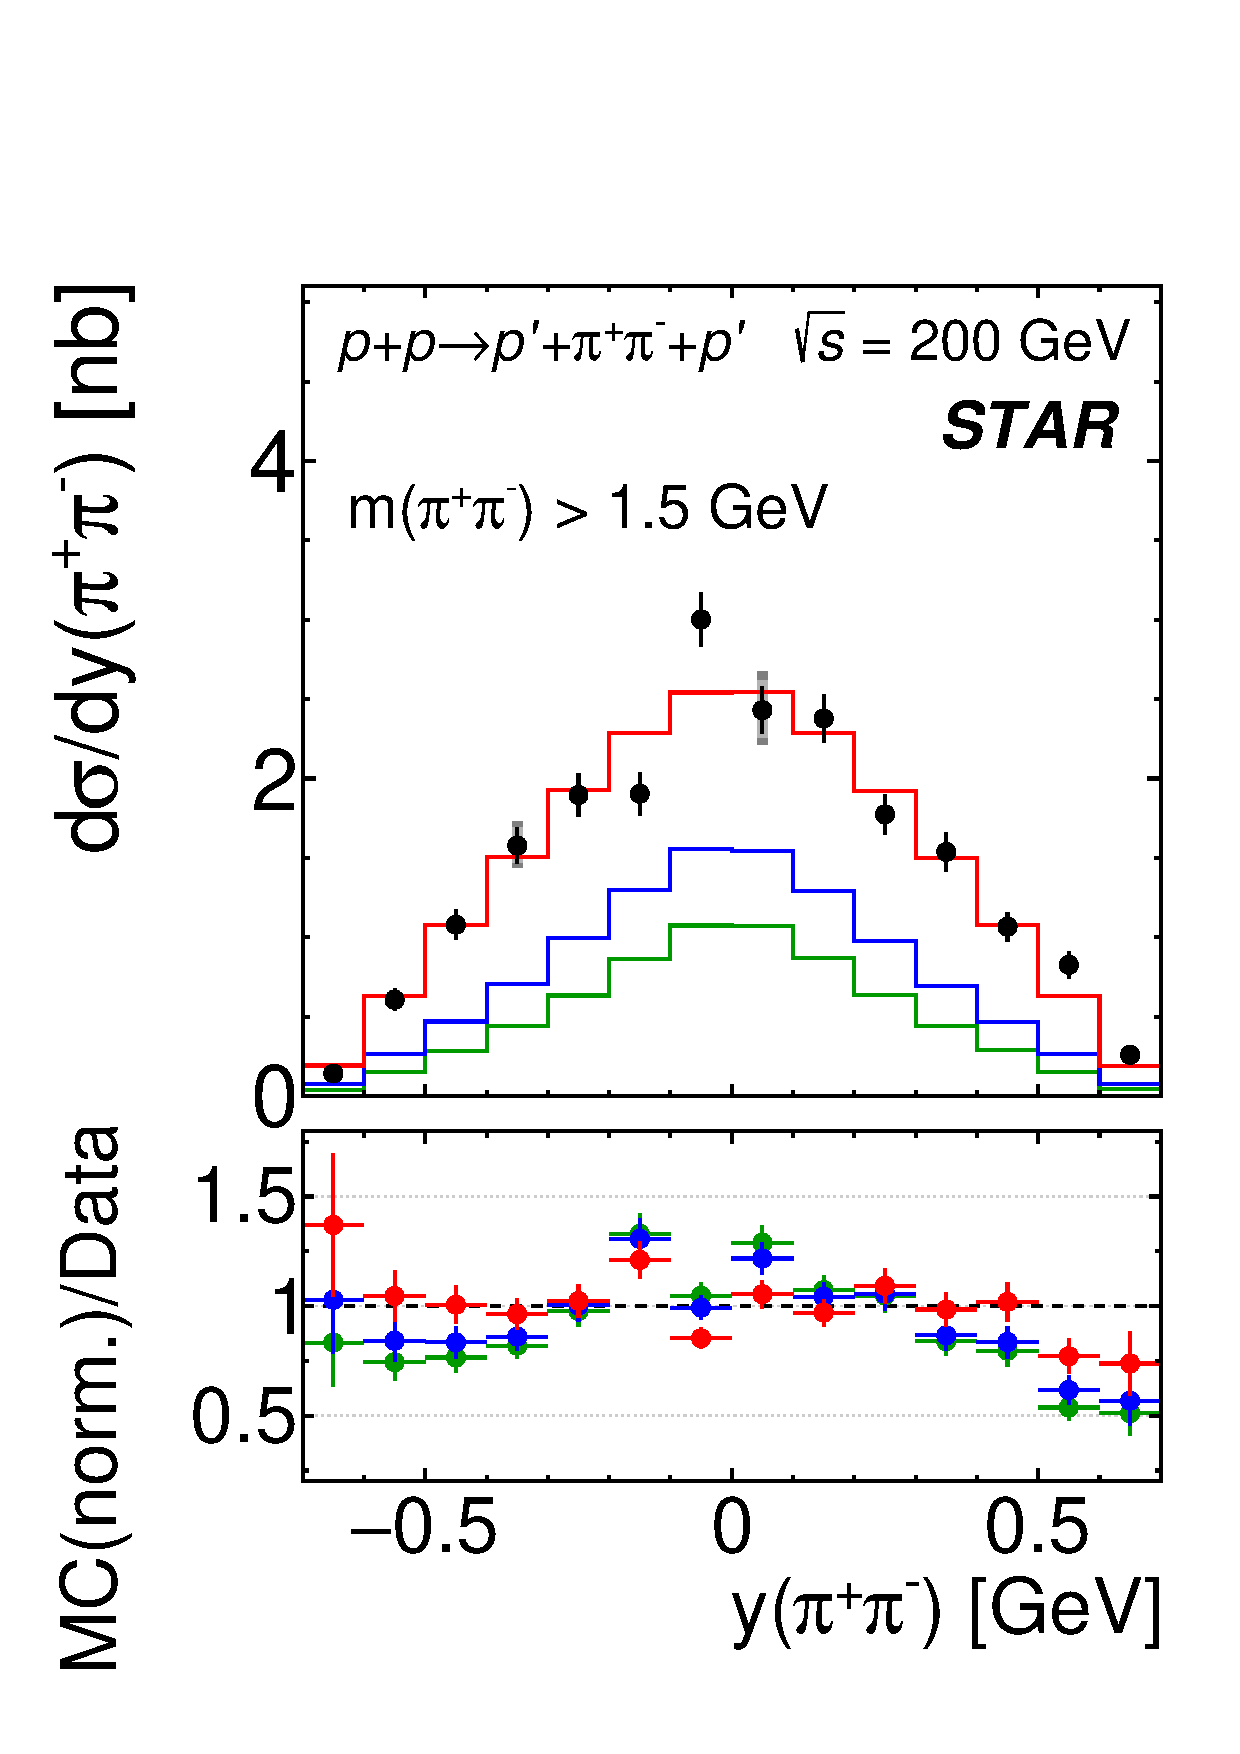
\includegraphics[width=.31\textwidth,page=1]{graphics/physicsResults/Ratio_FinalResult_Rapidity_pion_MassBin_3.pdf}
\hfill
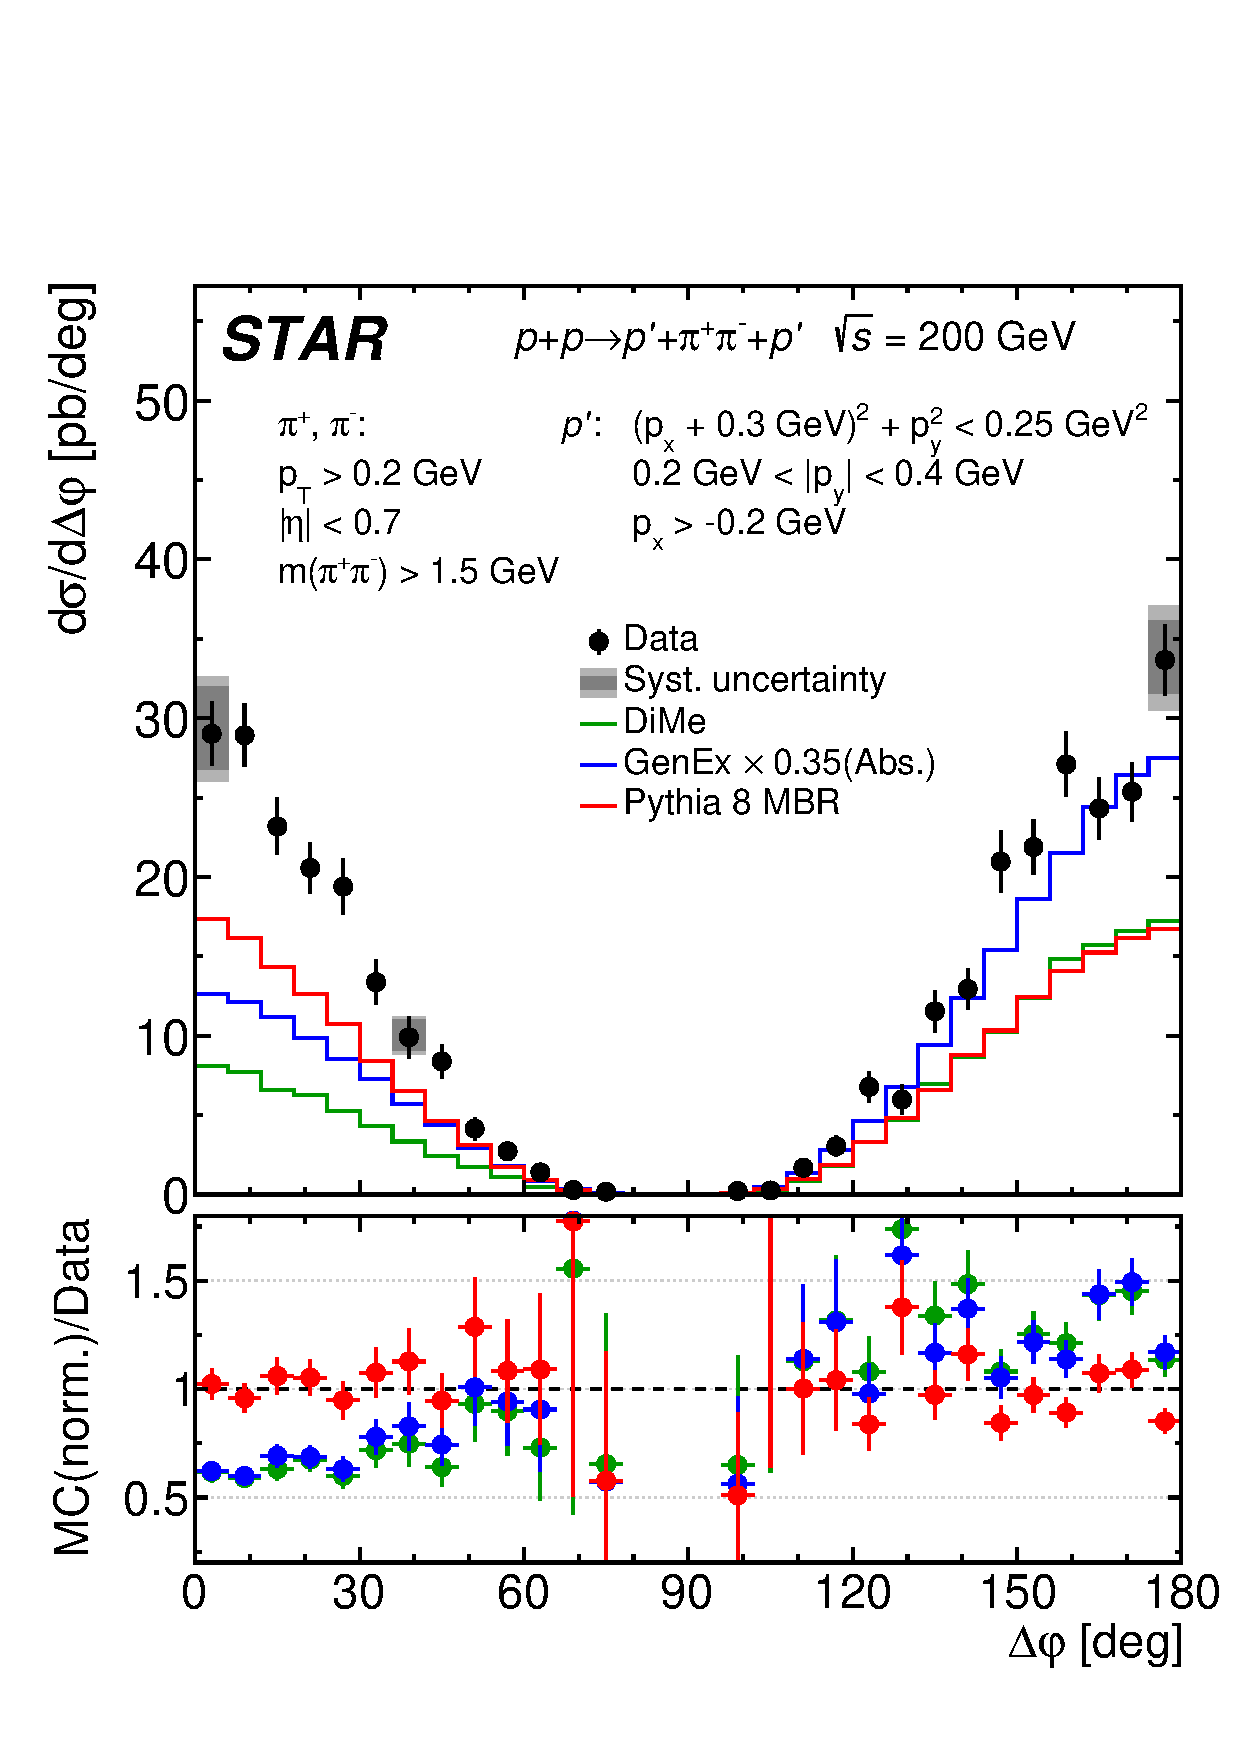
\includegraphics[width=.31\textwidth,page=1]{graphics/physicsResults/Ratio_FinalResult_DeltaPhi_pion_MassBin_3.pdf}
\hfill
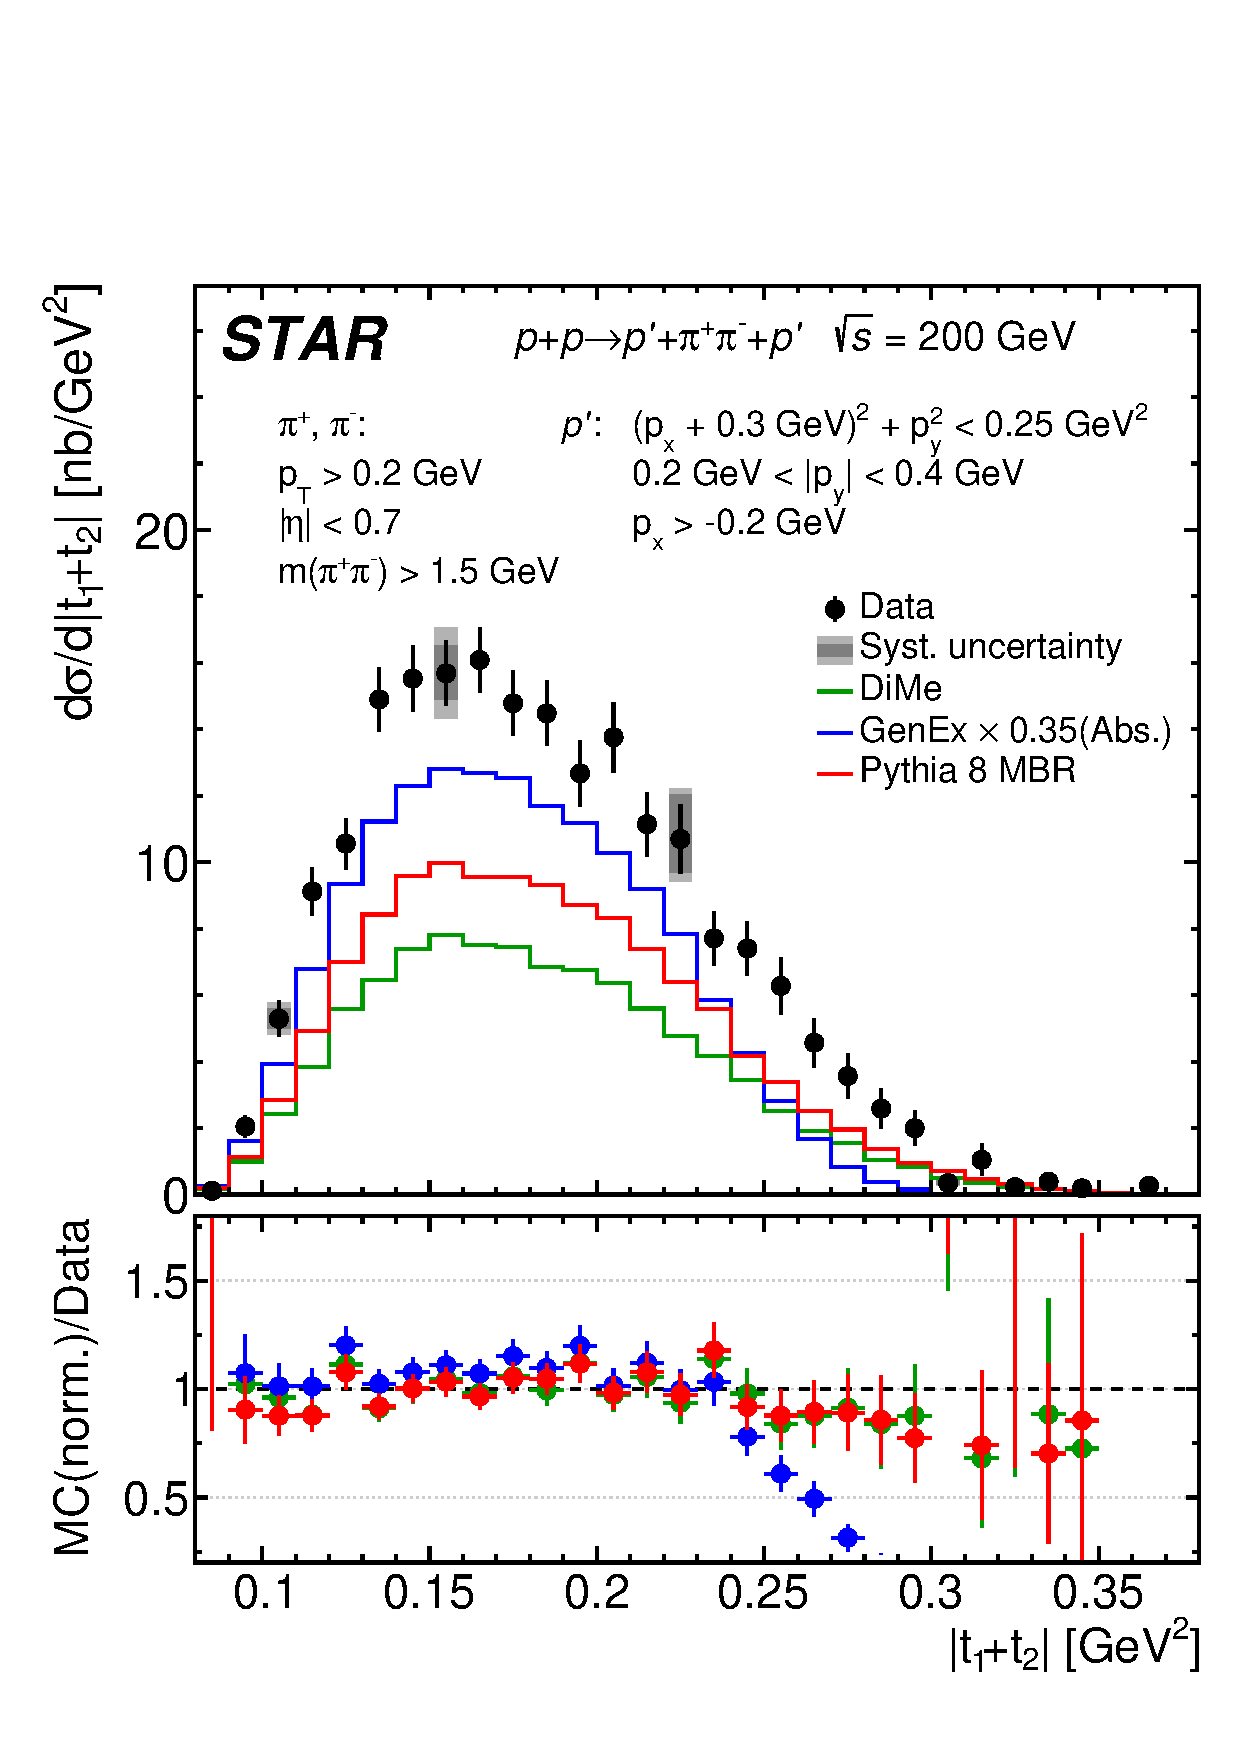
\includegraphics[width=.31\textwidth,page=1]{graphics/physicsResults/Ratio_FinalResult_MandelstamTSum_pion_MassBin_3.pdf}
%
\caption{Differential cross sections for CEP of $\pi^+\pi^-$ pairs as a function of the rapidity of the pair (left column) difference of azimuthal angles of the forward scattered protons (middle column) and of the sum of the squares of the four-momenta losses in the proton vertices (right column) measured in the fiducial region explained on the plots, separately for three ranges of the $\pi^+\pi^-$ pair invariant mass: $m<1$ GeV (top), $1<m<1.5$ GeV (middle) and $m>1.5$ GeV (bottom). Data are shown as solid points with error bars representing the statistical uncertainties. The typical systematic uncertainties are shown as gray boxes for only few data points as they are almost fully correlated between neighboring bins. Predictions from MC models GenEx, DiMe and MBR are shown as histograms. In the lower panels the ratios of the MC predictions scaled to data and the data are shown.}
\label{results_4}
\end{figure}
%
%\FloatBarrier
%
\begin{figure}[h]
\centering
\hspace*{5pt}
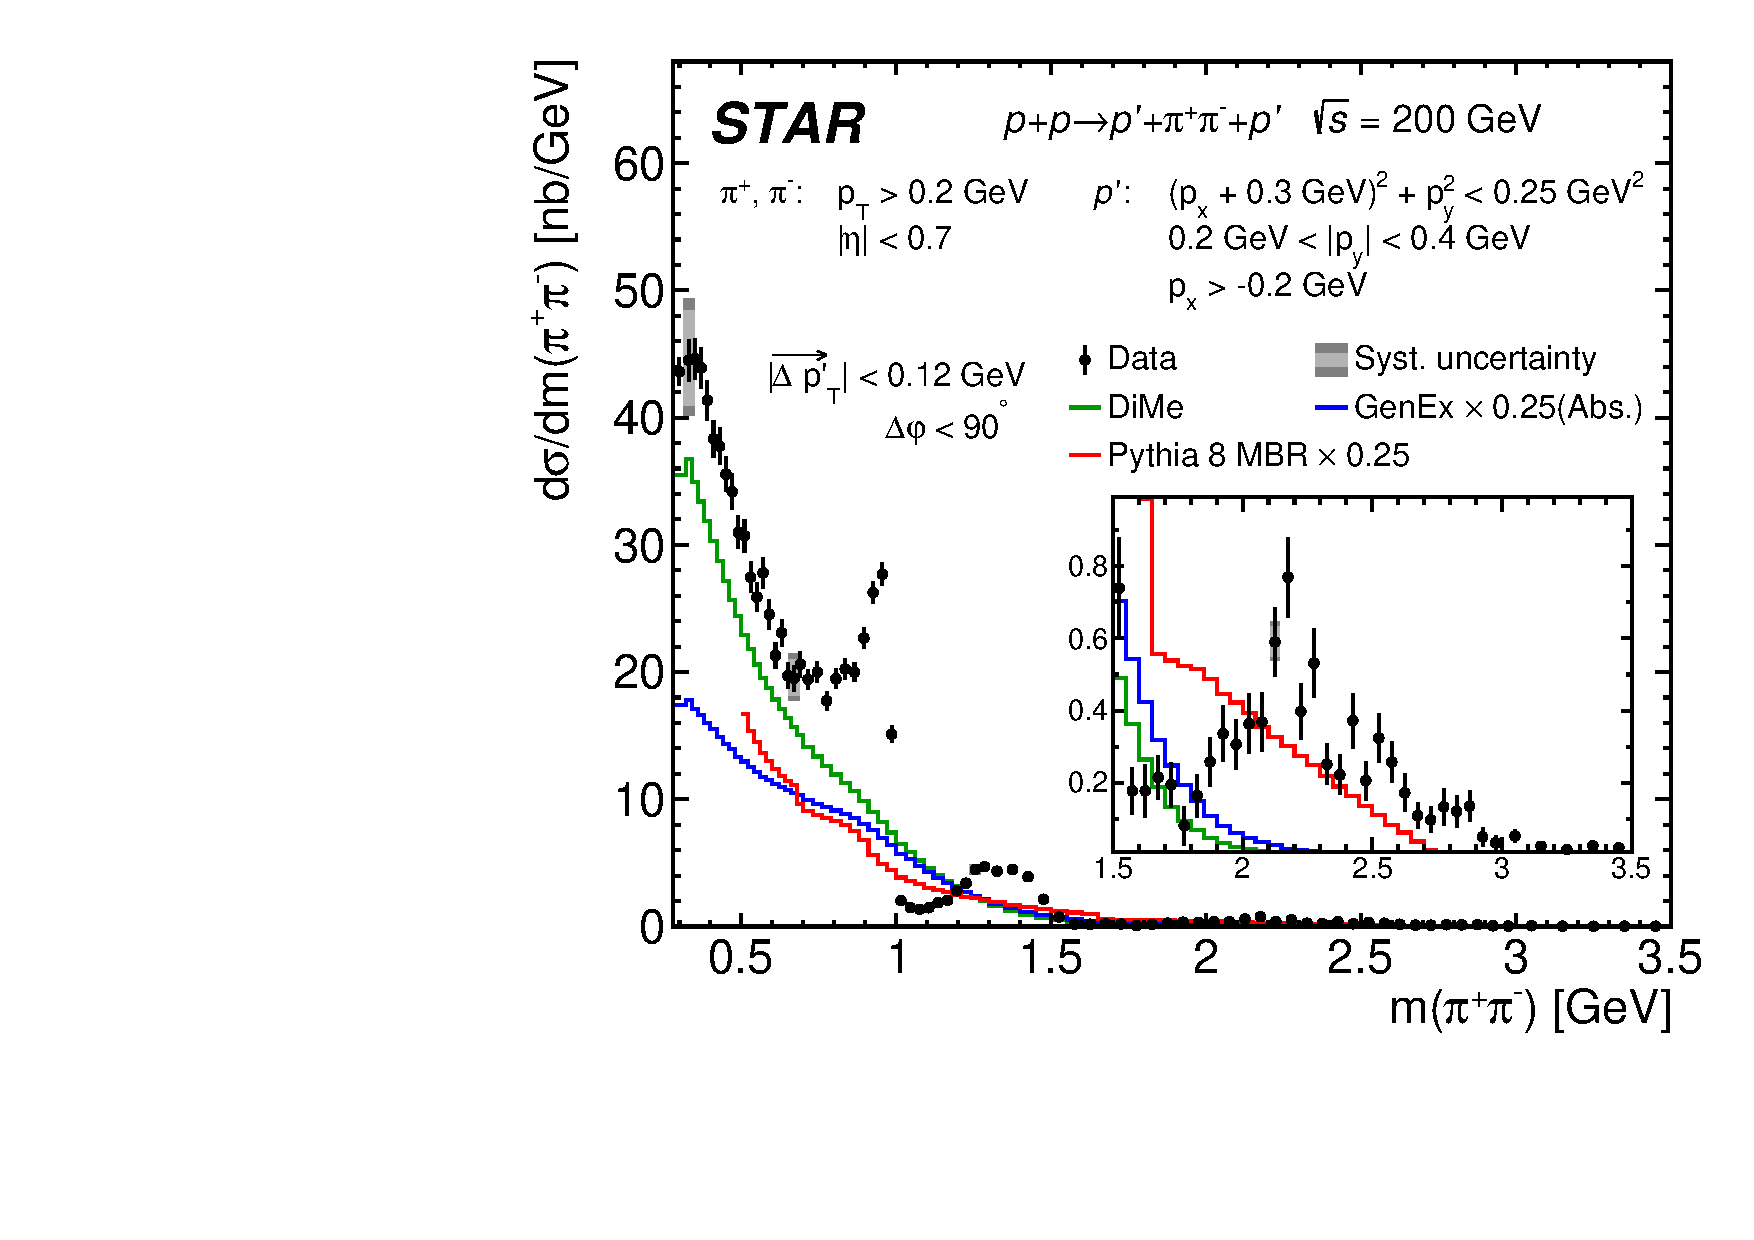
\includegraphics[width=.46\textwidth,page=1]{graphics/physicsResults/FinalResult_InvMass_pion_SmallDpt_DeltaPhiLessThan90.pdf}
\hfill
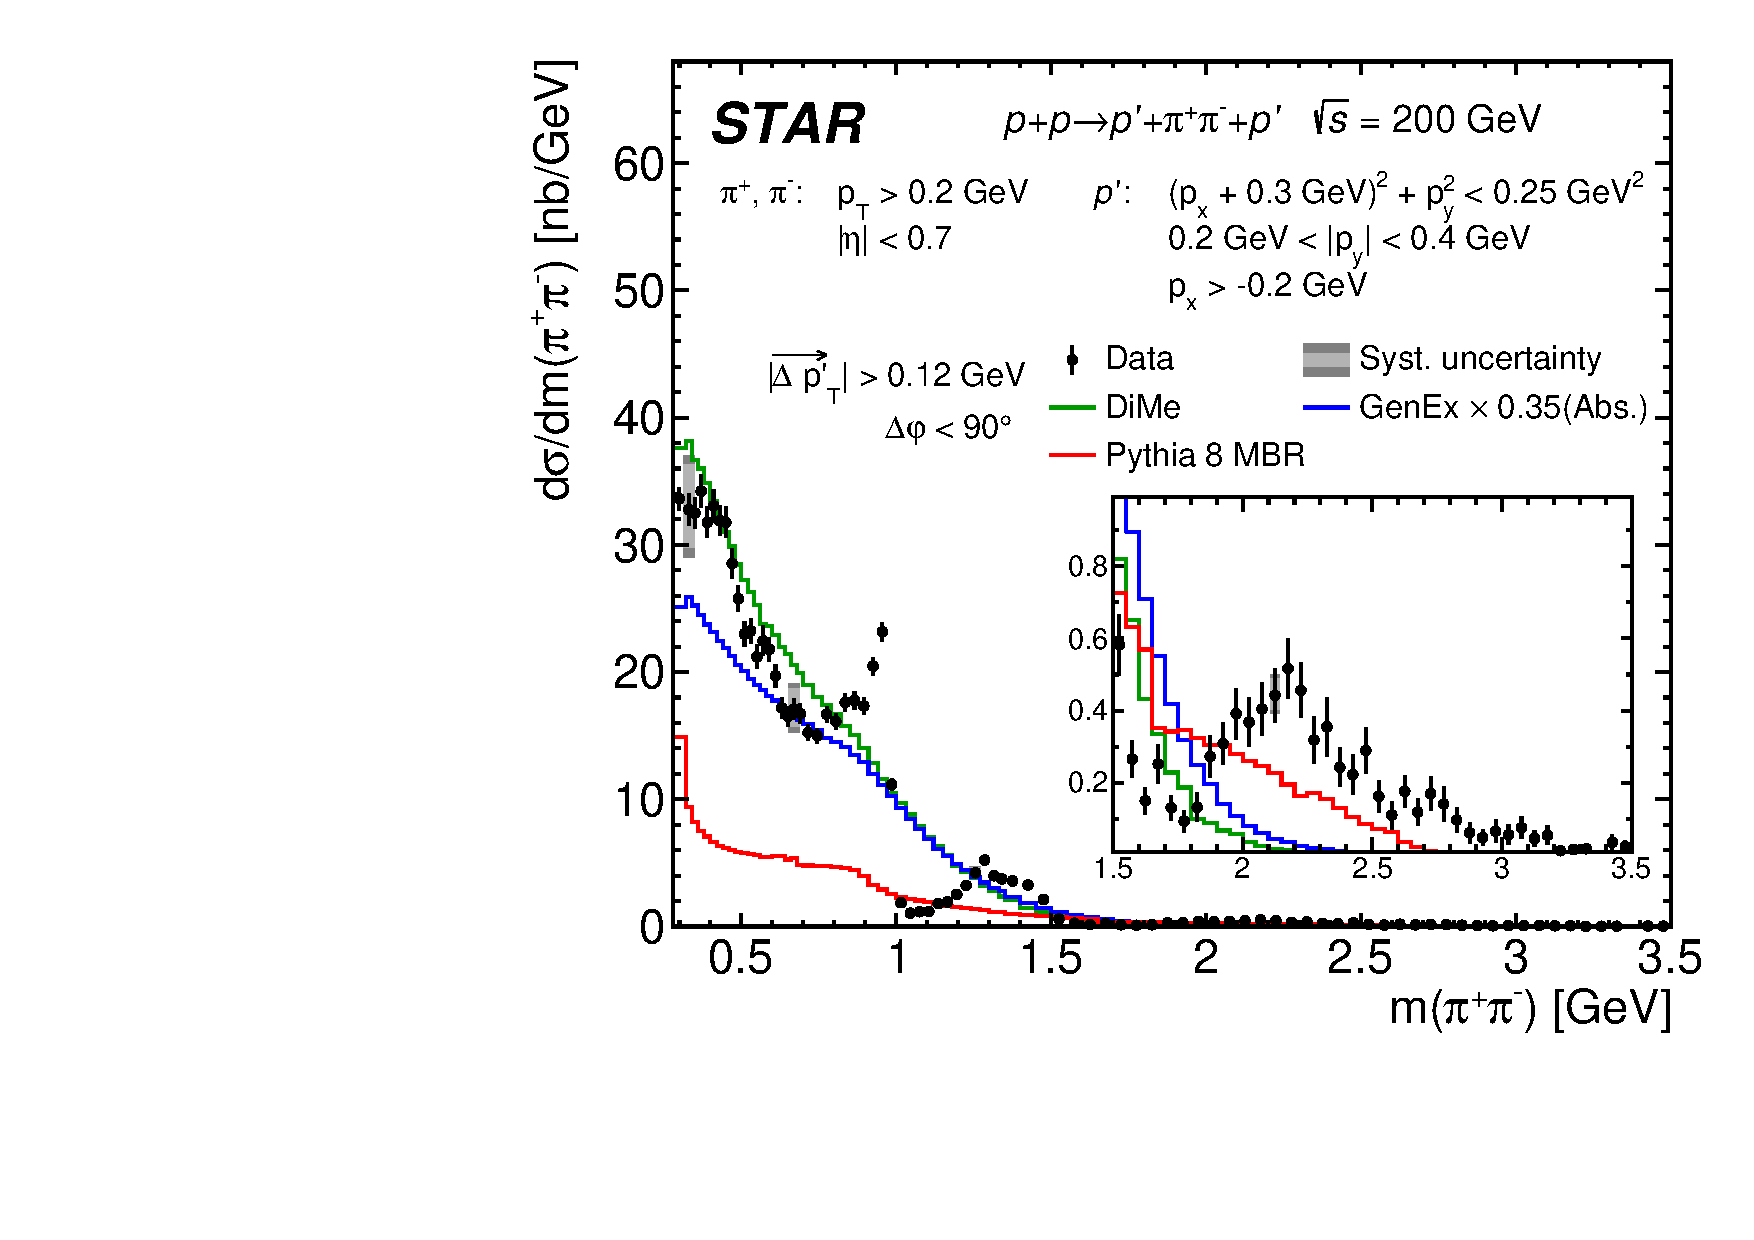
\includegraphics[width=.46\textwidth,page=1]{graphics/physicsResults/FinalResult_InvMass_pion_LargeDpt_DeltaPhiLessThan90.pdf}
\hspace*{5pt}
%
\caption{Differential cross sections $d\sigma/dm(\pi^+\pi^-)$ for CEP of $\pi^+\pi^-$ pairs in two $|\vec{p}_{1,T}^{\,\prime}-\vec{p}_{2,T}^{\,\prime}|$ regions: $|\vec{p}_{1,T}^{\,\prime}-\vec{p}_{2,T}^{\,\prime}|<0.12$ GeV (left) and $|\vec{p}_{1,T}^{\,\prime}-\vec{p}_{2,T}^{\,\prime}|>0.12$ GeV (right)  in the fiducial region and $\Delta\phi<90$ degree. There is no difference for two $|\vec{p}_{1,T}^{\,\prime}-\vec{p}_{2,T}^{\,\prime}|$ regions. Data are shown as solid points with error bars representing the statistical uncertainties. The typical systematic uncertainties are shown as gray boxes for only few data points as they are almost fully correlated between neighboring bins. Predictions from MC models GenEx, DiMe and MBR are shown as histograms.}
\label{results_5}
\end{figure}


% We have also studied angular distributions of the charged particles produced in the final state. This can be done in various reference frames. However, for an easy comparison with theoretical predictions we use here the Collins-Soper \cite{cs_frame} reference frame also used e.g. in Ref.~\cite{lebiedowicz_3}. Collins-Soper frame is the centre-of-mass frame of the charged particles pair with the $z$-axis making equal angles with the beam protons momenta which in addition define the new $x-z$ plane. It can be reached from the laboratory frame (proton-proton c.m.s.) in two steps. First, boost along the $z$-axis to an intermediate frame in which the pair longitudinal momentum is equal to zero. In this frame the beam protons momenta remain parallel to the $z$-axis and the transverse momentum of the pair remains unchanged. Second, boost in the direction of the transverse momentum of the pair, to get to the pair c.m.s. frame.
%
\begin{figure}[h]
\centering
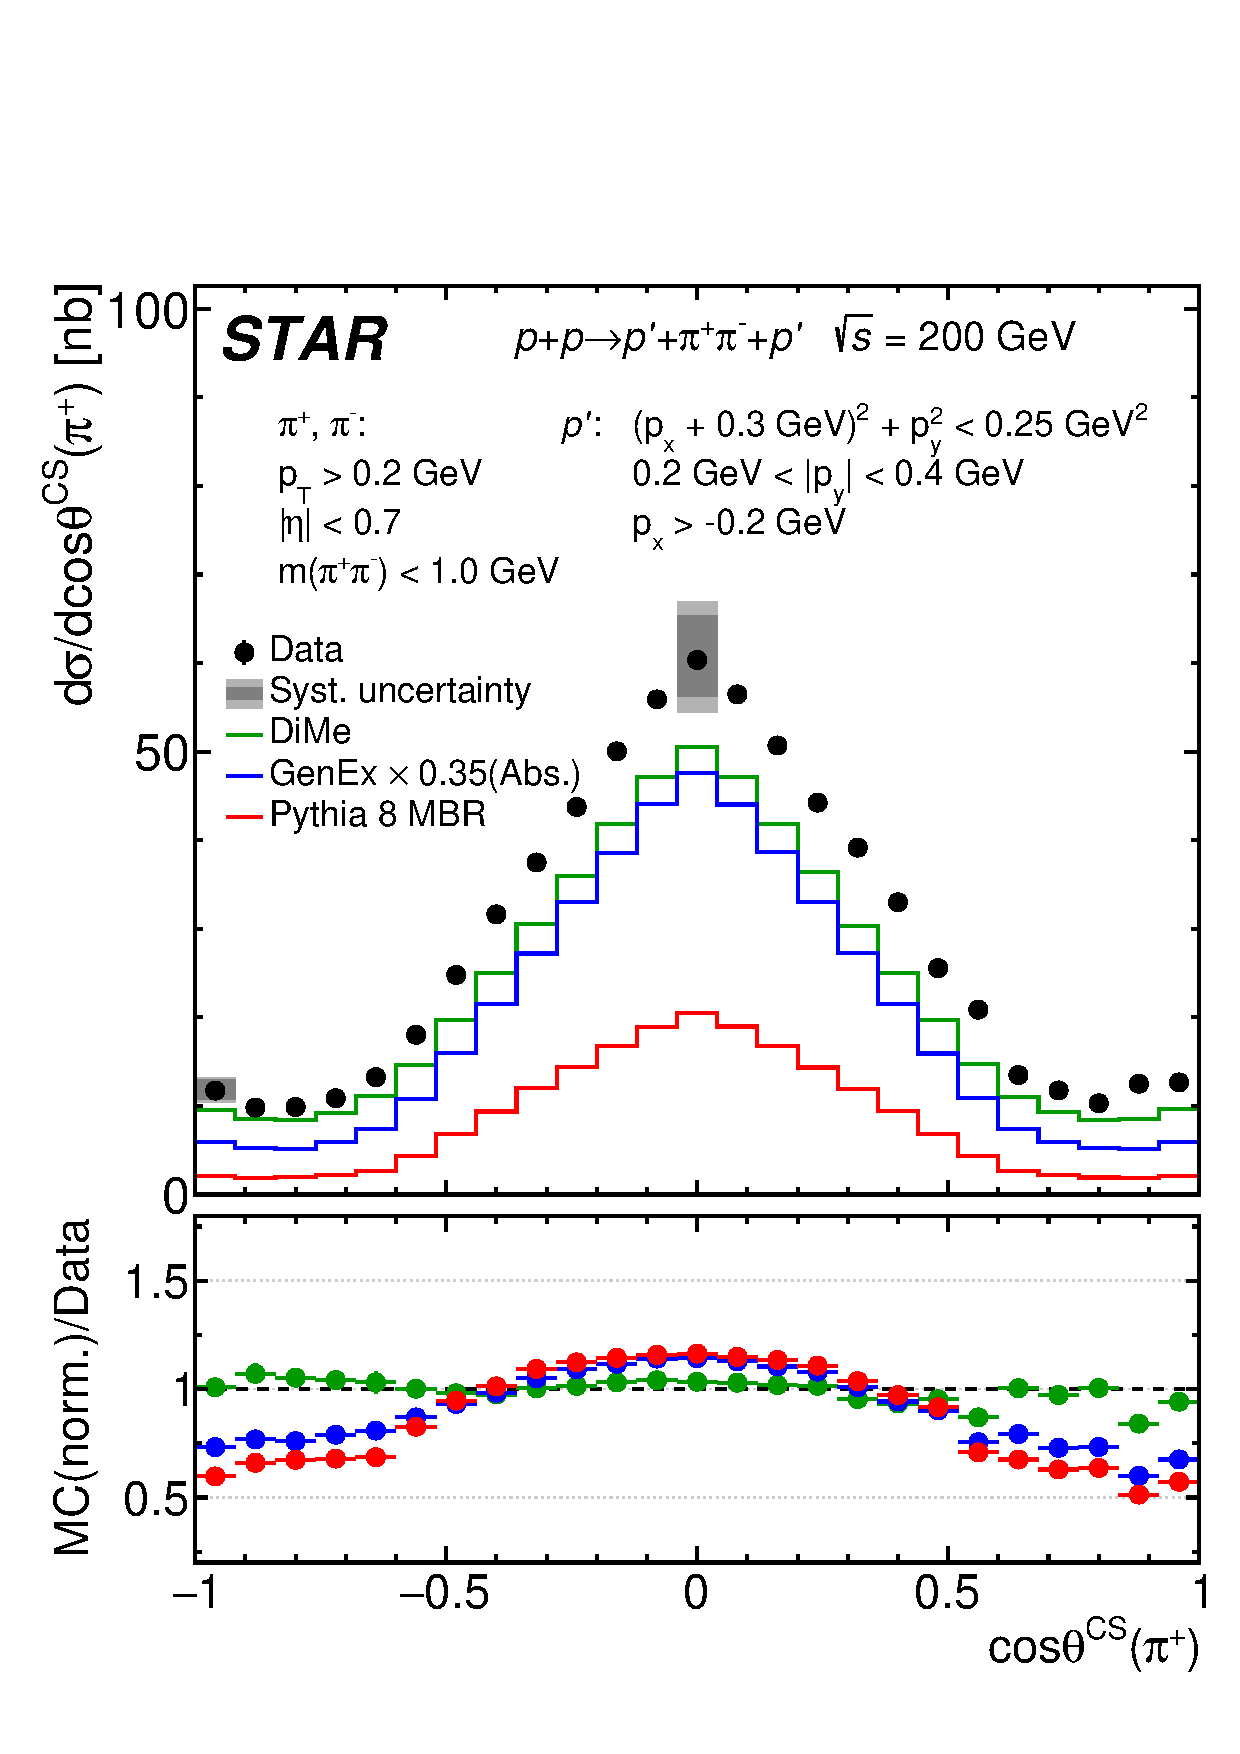
\includegraphics[width=.31\textwidth,page=1]{graphics/physicsResults/Ratio_FinalResult_CosThetaCS_pion_MassBin_1.pdf}
\hfill
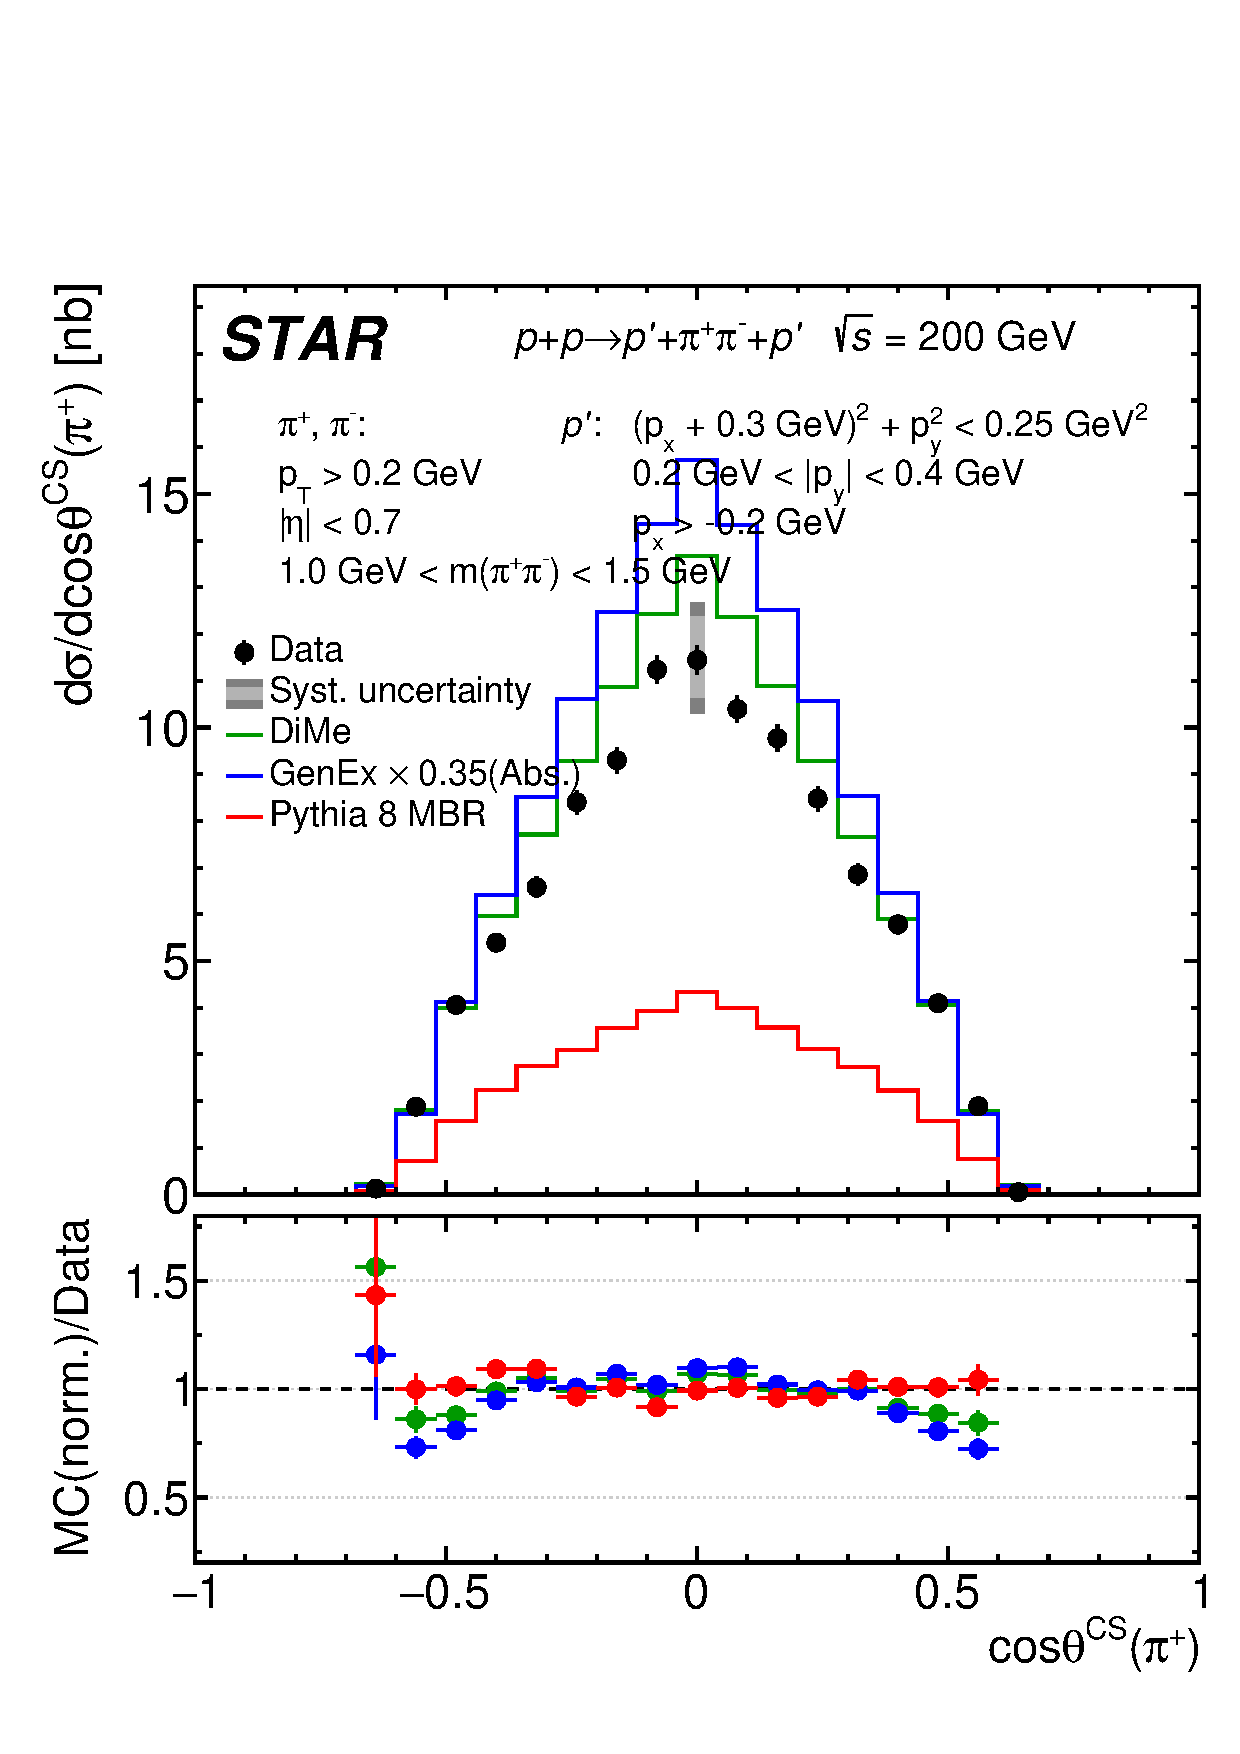
\includegraphics[width=.31\textwidth,page=1]{graphics/physicsResults/Ratio_FinalResult_CosThetaCS_pion_MassBin_2.pdf}
\hfill
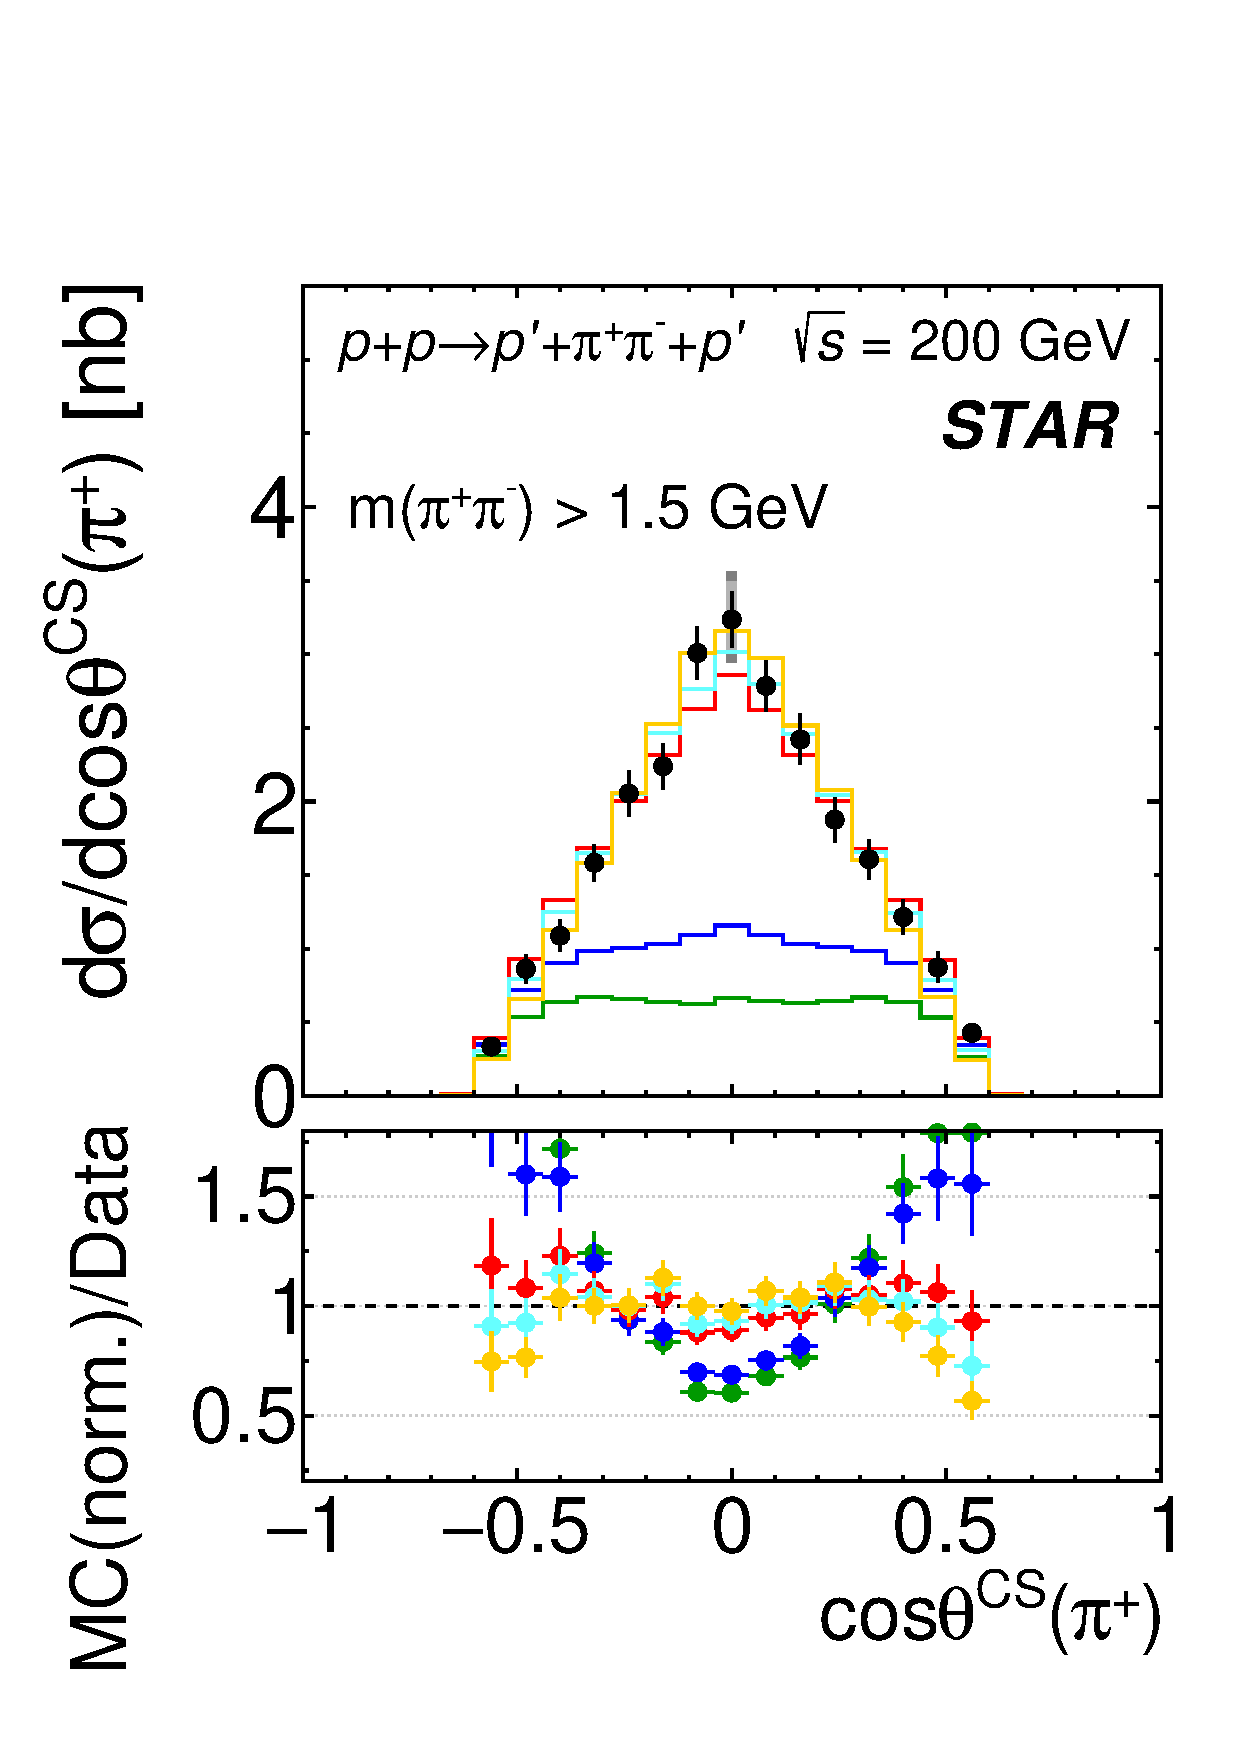
\includegraphics[width=.31\textwidth,page=1]{graphics/physicsResults/Ratio_FinalResult_CosThetaCS_pion_MassBin_3.pdf}
\newline
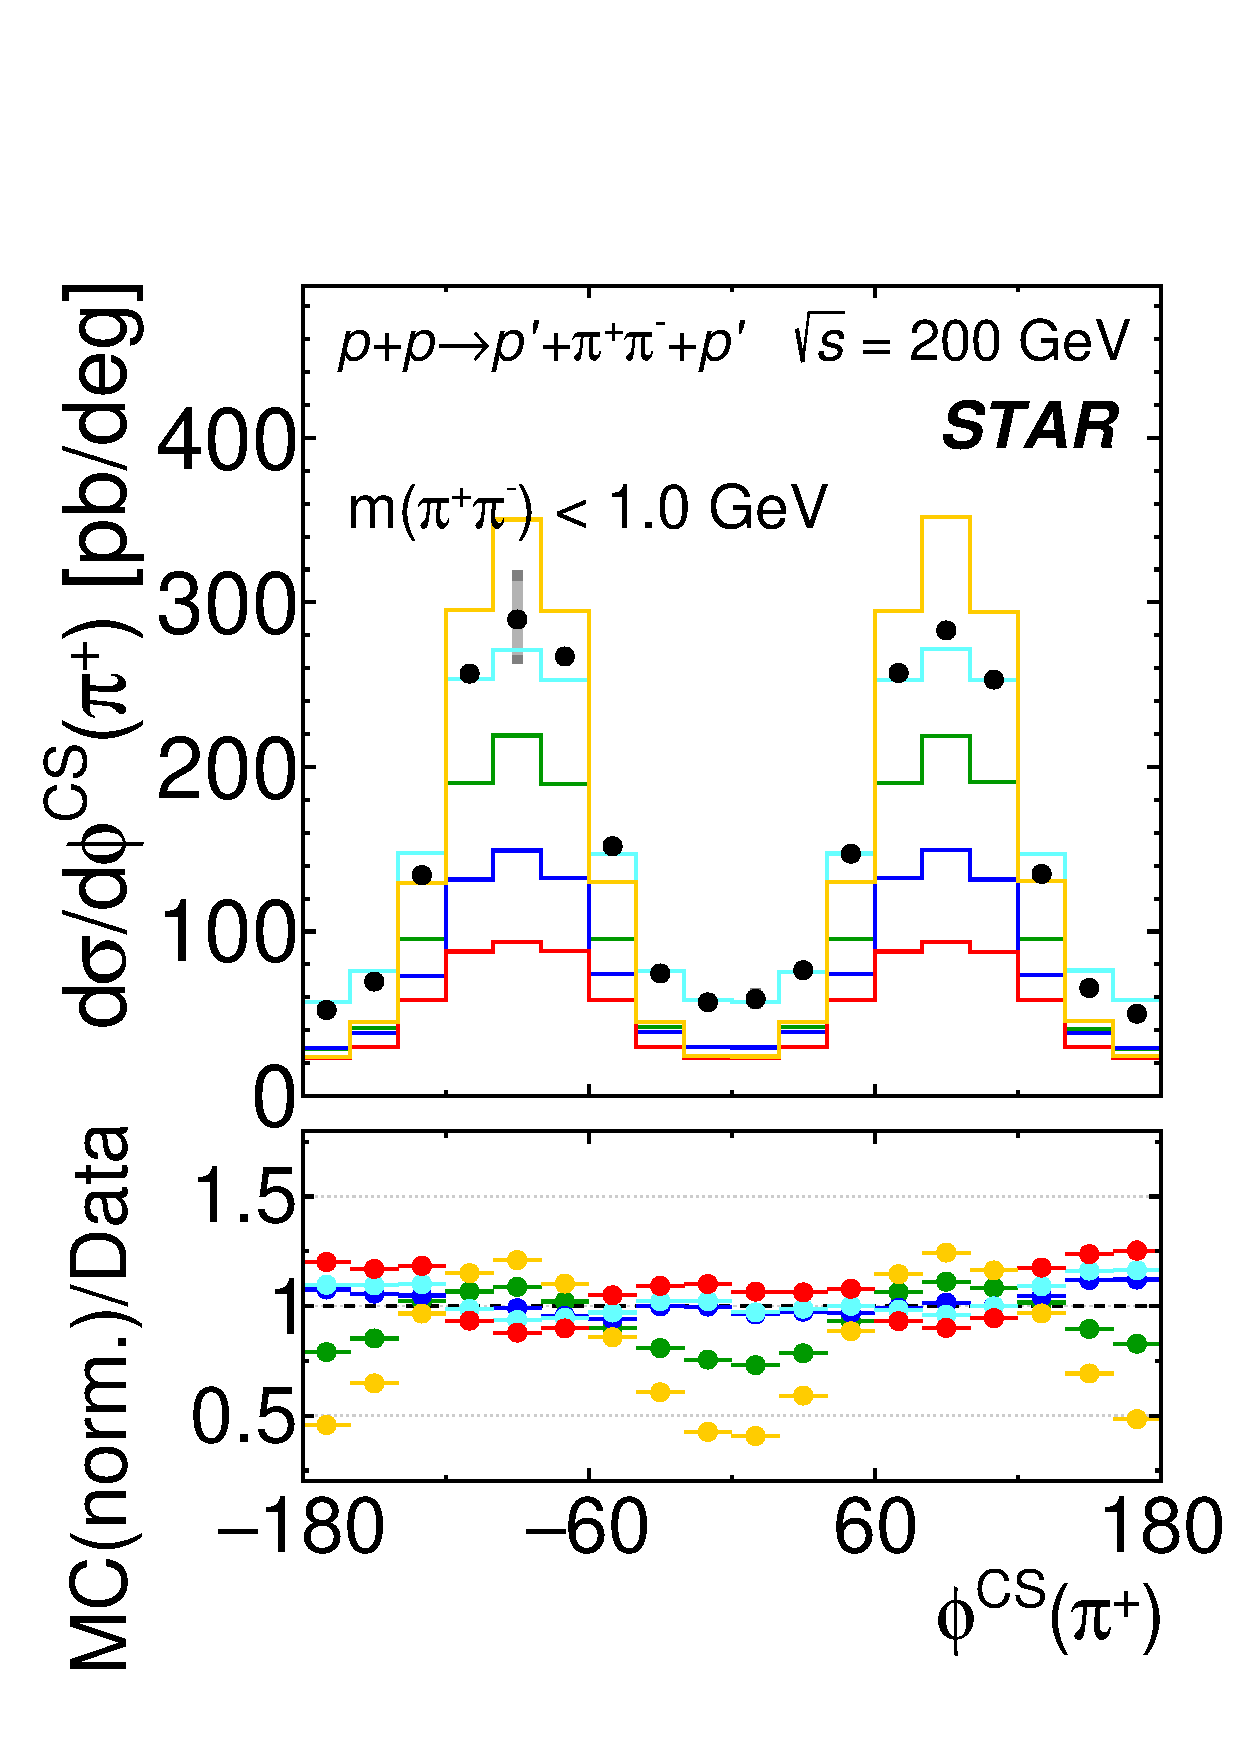
\includegraphics[width=.31\textwidth,page=1]{graphics/physicsResults/Ratio_FinalResult_PhiCS_pion_MassBin_1.pdf}
\hfill
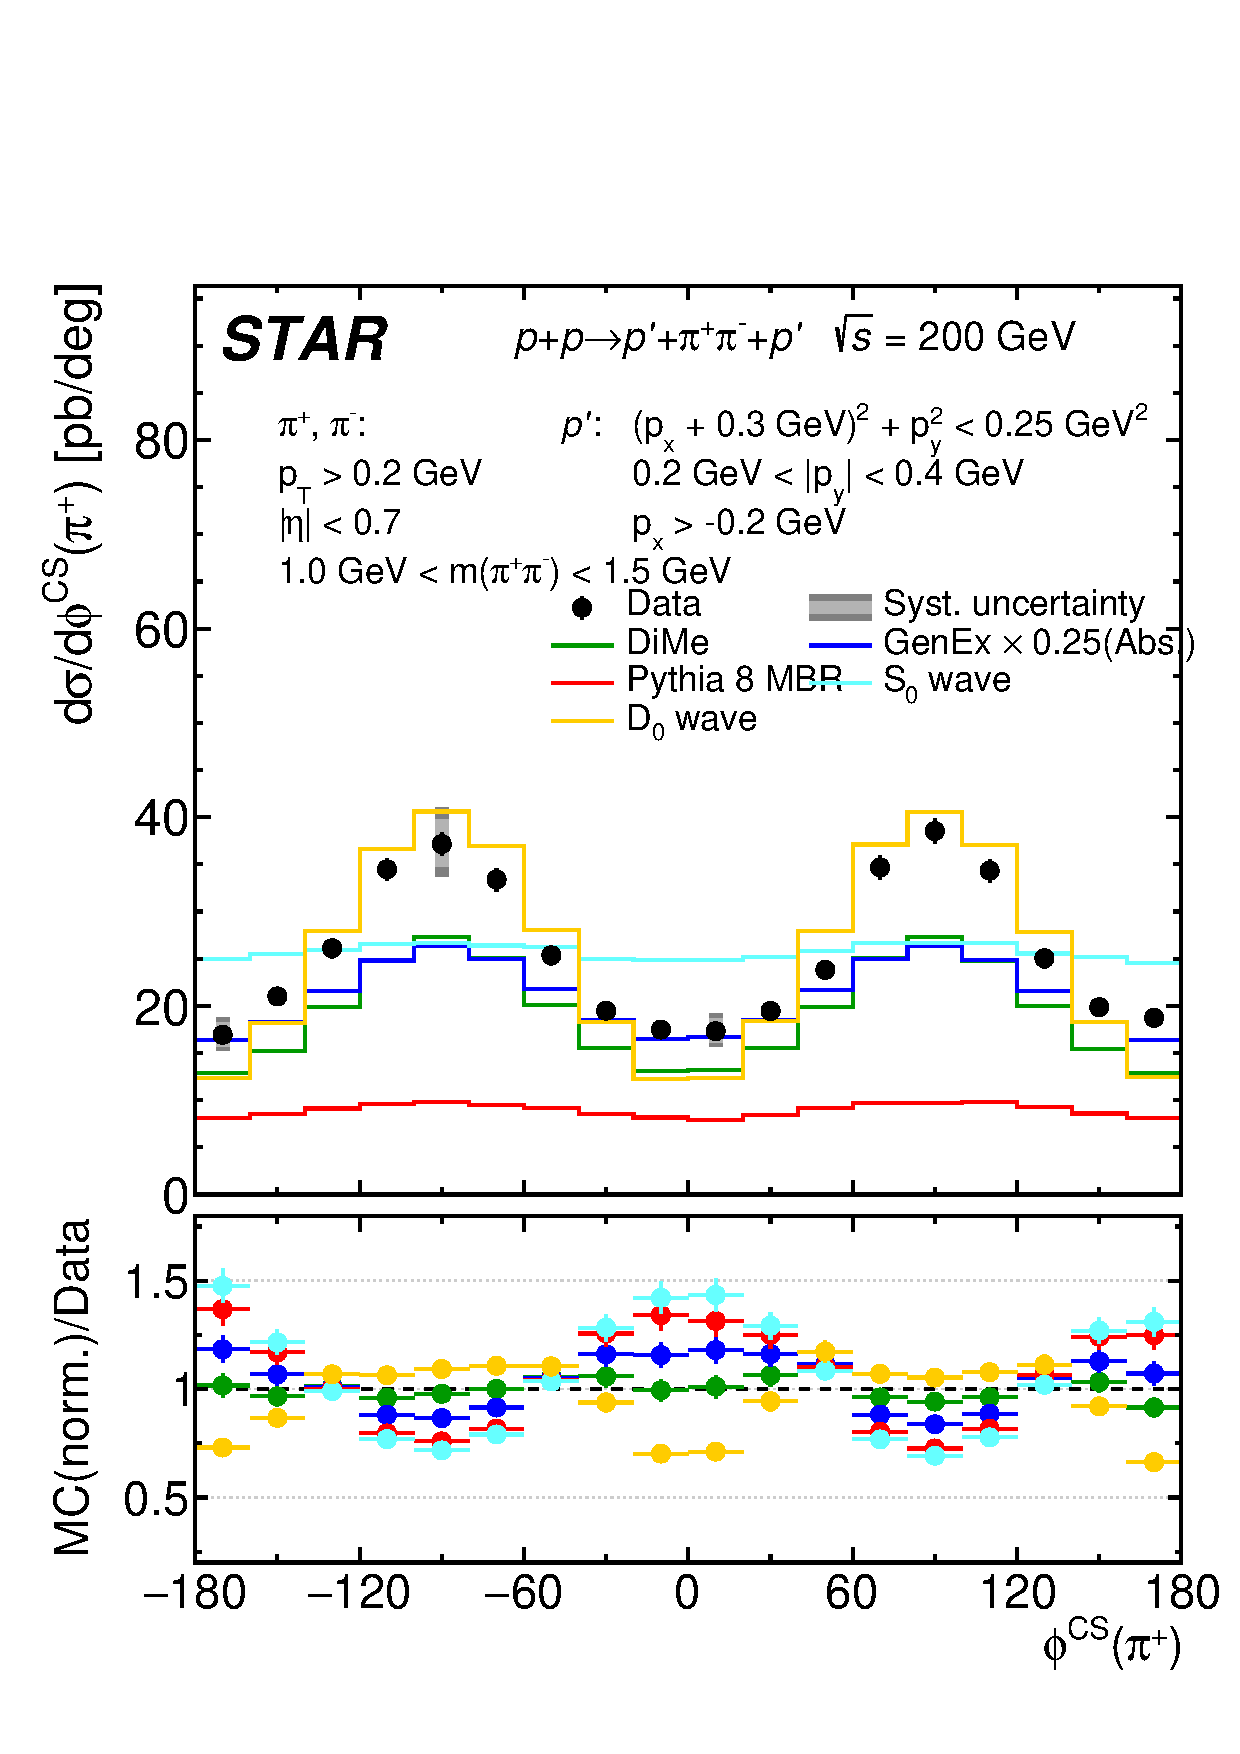
\includegraphics[width=.31\textwidth,page=1]{graphics/physicsResults/Ratio_FinalResult_PhiCS_pion_MassBin_2.pdf}
\hfill
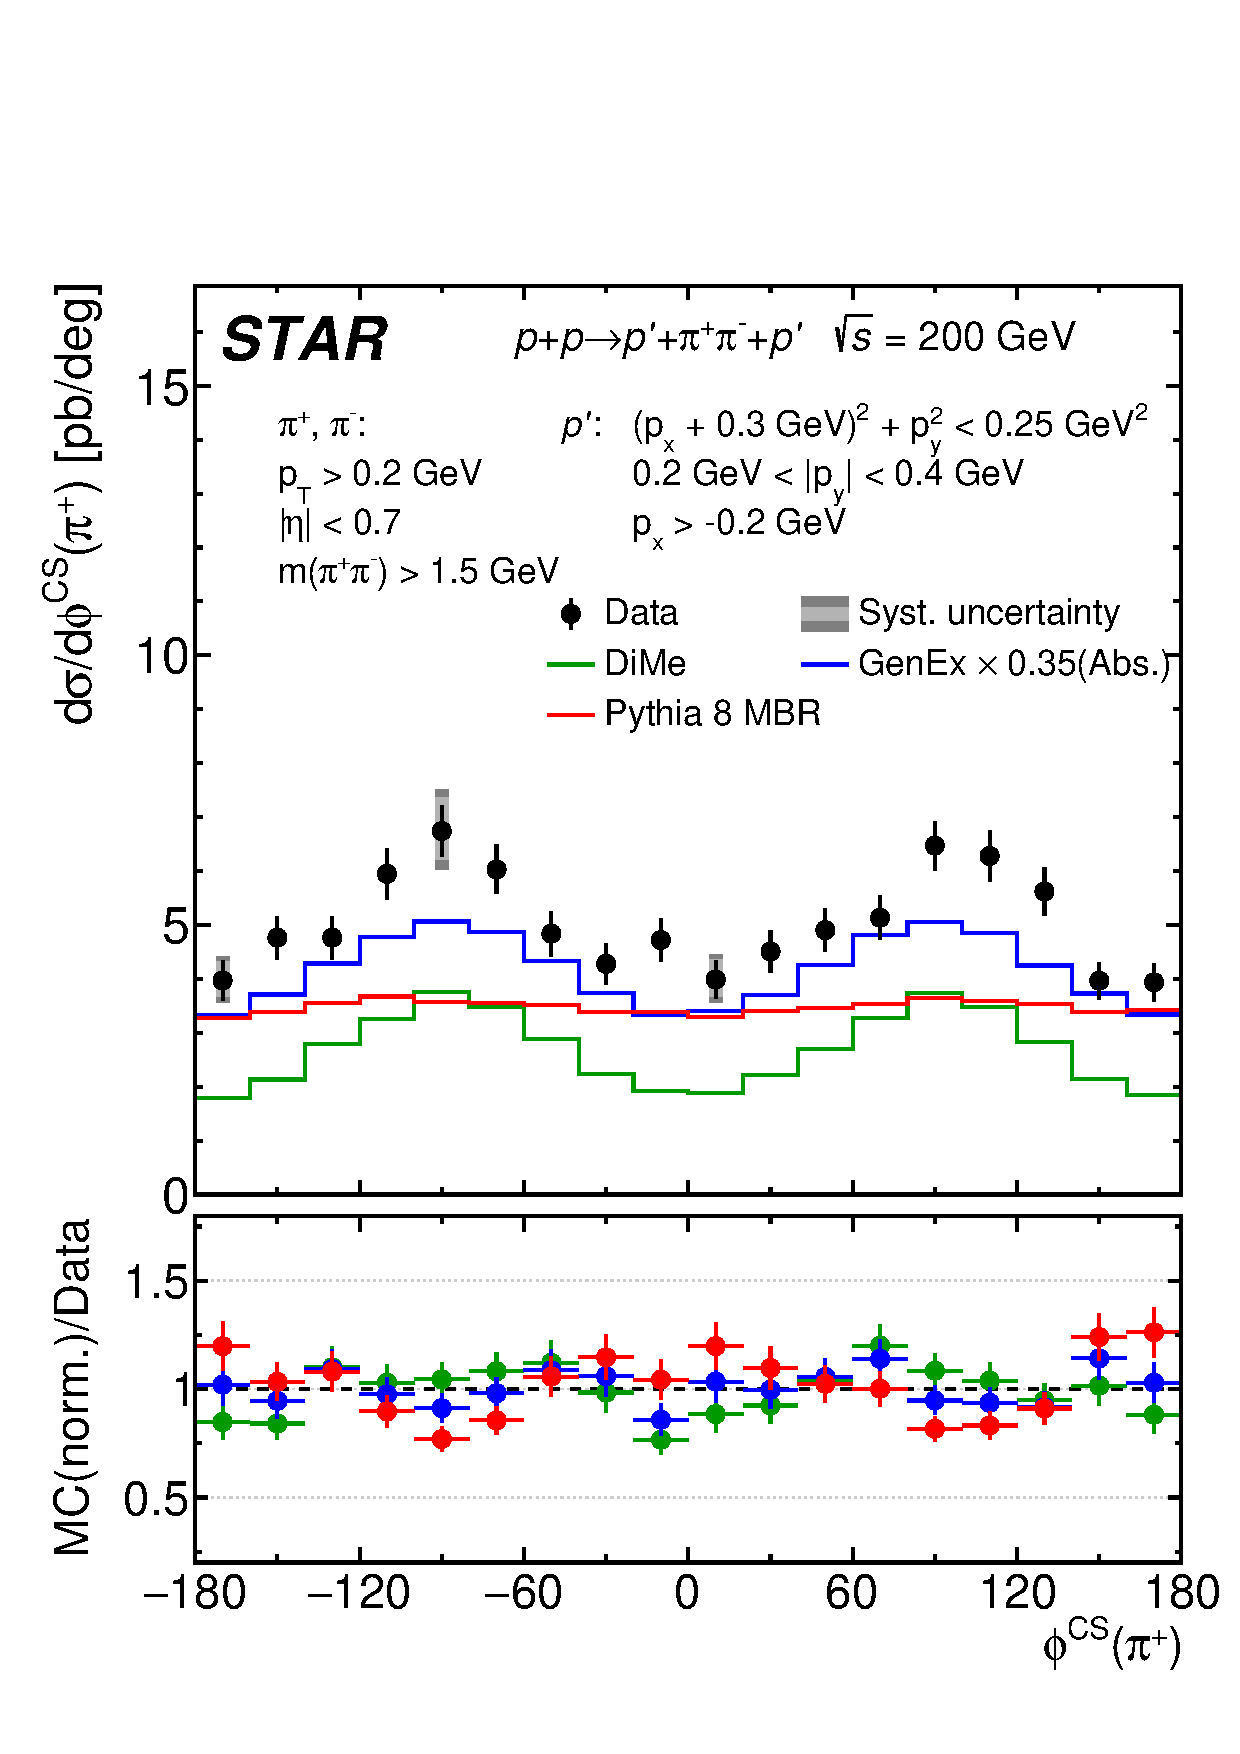
\includegraphics[width=.31\textwidth,page=1]{graphics/physicsResults/Ratio_FinalResult_PhiCS_pion_MassBin_3.pdf}
%
\caption{Differential cross sections for CEP of $\pi^+\pi^-$ pairs as a function of $\cos{\theta^\mathrm{CS}}$ (top) and of $\phi^\mathrm{CS}$ (bottom)  measured in the fiducial region explained on the plots, separately for three ranges of the $\pi^+\pi^-$ pair invariant mass: $m<1$ GeV (left column), $1<m<1.5$ GeV (middle column) and $m>1.5$ GeV (right column). Data are shown as solid points with error bars representing the statistical uncertainties. The typical systematic uncertainties are shown as gray boxes for only few data points as they are almost fully correlated between neighboring bins. Predictions from MC models GenEx, DiMe and MBR are shown as histograms. In the lower panels the ratios of the MC predictions scaled to data and the data are shown.}
\label{results_7}
\end{figure}
